\documentclass[11pt]{article}

\usepackage{url}
\usepackage[font=footnotesize,labelfont=bf]{caption}
\usepackage{graphicx}
\usepackage[scientific-notation=true]{siunitx}
\usepackage{subcaption}
\usepackage{setspace}
\usepackage[top=0.6 in, bottom=0.7 in, left=0.7in, right=0.7in]{geometry}
\usepackage{blindtext}
\usepackage[utf8]{inputenc}
\usepackage{setspace}
\usepackage{vector}
\usepackage{amsmath}
\usepackage{empheq}
\usepackage{amssymb}
\usepackage{tgtermes}
\usepackage{gensymb}
\DeclareGraphicsExtensions{.pdf,.png,.jpg}
\usepackage{epstopdf}
\usepackage[singlelinecheck=false]{caption}
\usepackage[hyperfootnotes=false, pdfnewwindow, colorlinks=true]{hyperref}
\usepackage[title]{appendix}
\usepackage[section]{placeins}
\usepackage{float}
\usepackage{xcolor}

\AtBeginDocument{% optionally set colors to your liking
  \hypersetup{
    urlcolor=blue,
    citecolor=blue,
    linkcolor=blue,
  }%
}


\begin{document}

%GLOBAL VARIABLE DEFINITIONS
\newcommand{\hhodthrs}{-44.5 mV }       %define HMS Hodo threholds in case they change later on, only change this line!!!
\newcommand{\hhodgate}{60 ns }
\newcommand{\hPrShLo}{-40 mV }
\newcommand{\hPrShHi}{-60 mV }
\newcommand{\hSHLo}{-45 mV }
\newcommand{\hPrShLogate}{30 ns }
\newcommand{\hPrShHigate}{30 ns }
\newcommand{\hSHLogate}{30 ns }
\newcommand{\hcerthrs}{-50 mV }
\newcommand{\hcergate}{30 ns }

\newcommand{\shodthrs}{-30 mV }
\newcommand{\quartzthrs}{-60 mV }
\newcommand{\shodgate}{60 ns } 
\newcommand{\sngcthrs}{-50 mV}
\newcommand{\sngcgate}{30 ns}
\newcommand{\shgcthrs}{-50 mV}
\newcommand{\shgcgate}{30 ns}
\newcommand{\saerthrs}{-50 mV}
\newcommand{\saergate}{30 ns}
\newcommand{\comment}[1]{}

\begin{center}
  \vspace*{\stretch{1}}
  \textbf{\noindent \large \textcolor{red}{DISCLOSURE: \\ THE ELECTRONIC DIAGRAMS SHOWN IN THE MAIN TEXT ARE UPDATED AND CORRESPOND TO THE ELECTRONICS DIAGRAMS USED IN A1N/D2N EXPERIMENTS AS OF FALL 2019 - FALL 2020. THE CHANGES ARE MINOR, HOWEVER, IF YOUR EXPERIMENT RAN BEFORE FALL 2019, PLEASE REFER TO SECTION 6 (PAGE 17) OF THIS DOCUMENT FOR CLARIFICATION OF THE CHANGES MADE.}}
  \vspace*{\stretch{1}}
\end{center}
\newpage

\title{\LARGE \bf{Hall C 12 GeV Trigger Set-Up}}

\author{Carlos Yero \\ email \href{mailto:cyero002@fiu.edu}{cyero002@fiu.edu}}

\maketitle



%*****************************************************************************************************************************************************
\section{Detector Electronics Racks and Patch Panel Diagrams}
The majority of the detector electronics in the HMS/SHMS detector huts are read out in the Counting Room except for the HMS/SHMS Drift
Chambers and the SHMS Shower Counter signals which are read in their respective detector huts. In HMS/SHMS huts, the Drift
Chamber signals are output by 20-25 feet long ribbon cables which are read in the hut electronics rack (See Figure \ref{fig:hms_hut_rack}). On the SHMS
side, the Shower Counter consists of 224 signal cables which would take up most of the space available for other detectors
in the Counting Room, so they are read directly in the hut electronics rack.

\subsection{HMS Detector Hut}
The HMS Drift Chambers are read out through a VXS Crate (ROC3) in the detector hut electronics rack. The signals are carried through 16-channel ribbon cables
which are fed in various CAEN1190 TDC modules. The \textbf{TI} (or Trigger Interface) module at the front end of the crate distributes the readout
trigger throughout all modules in the crate and initiates data readout.
\begin{figure}[h!]
  \centering
  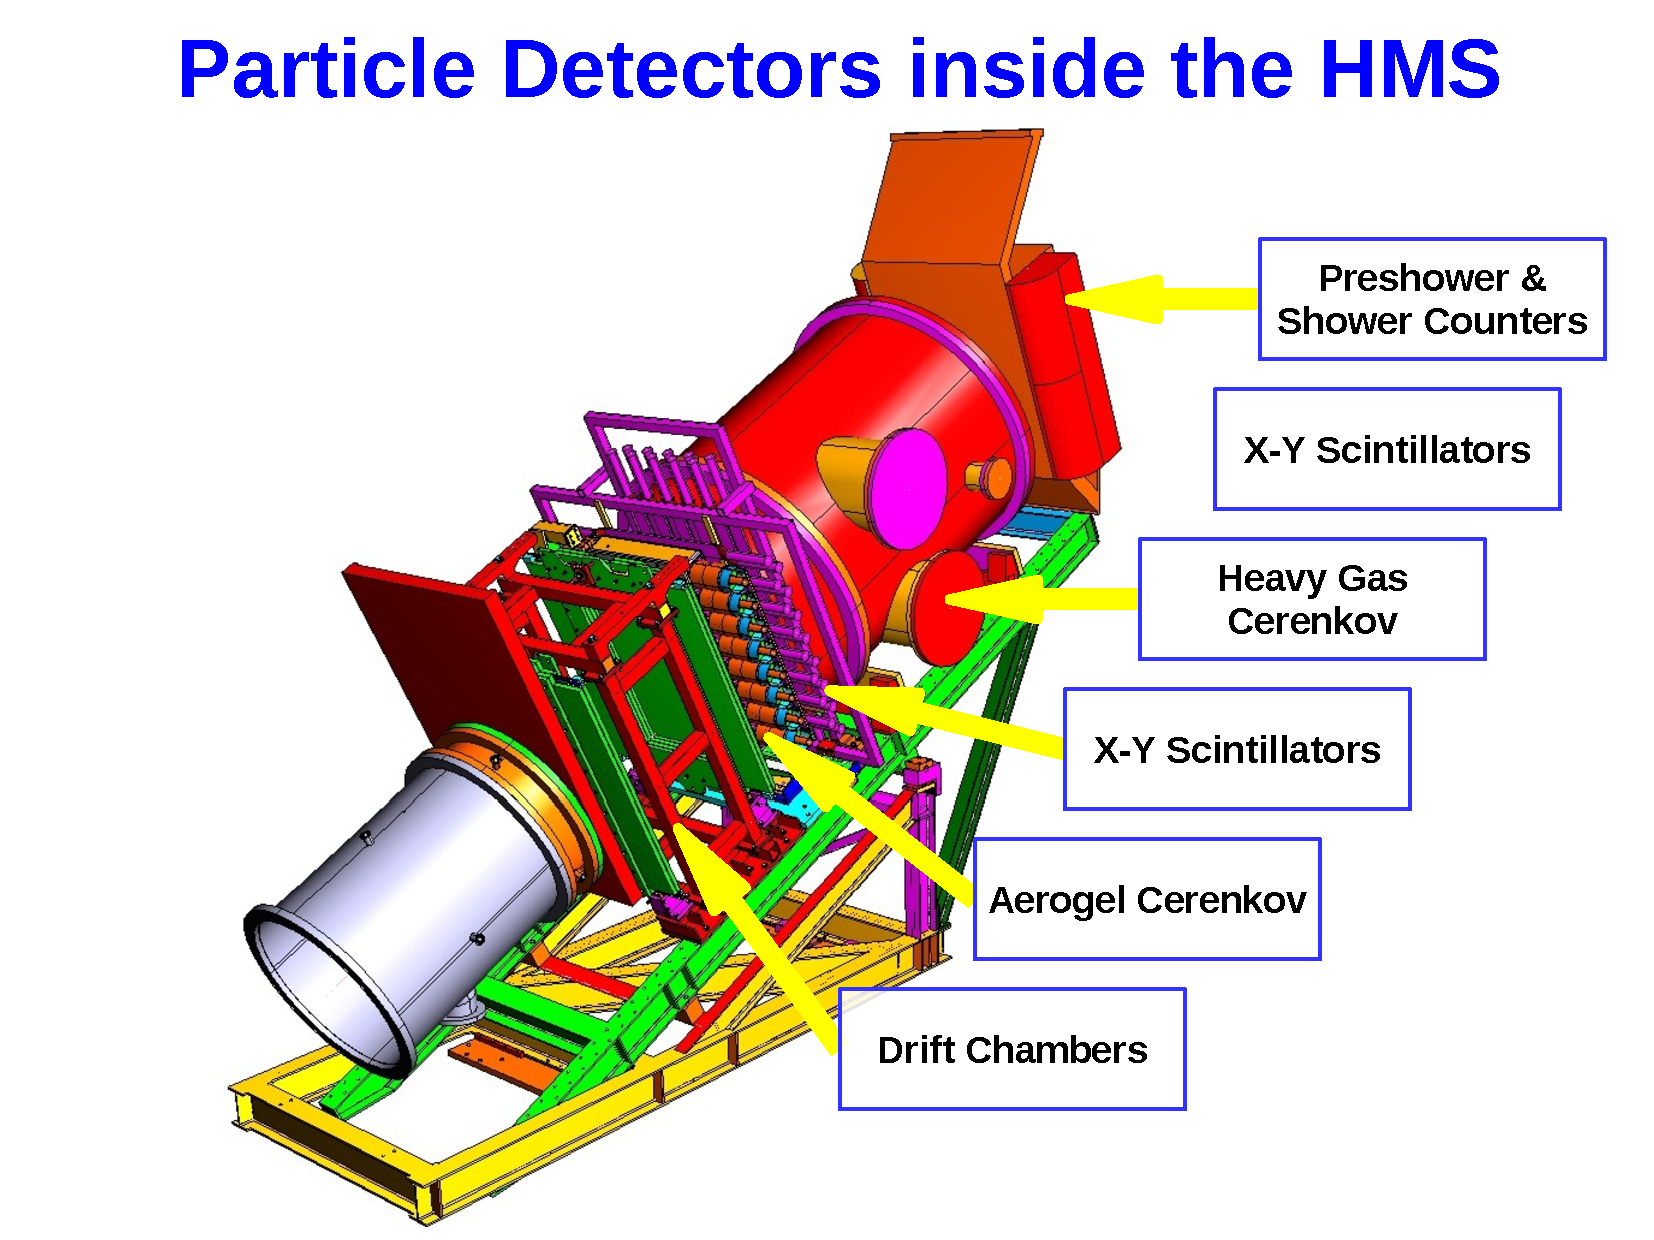
\includegraphics[width=5.0in, height=4.0in]{../HMS_stack.pdf}
  \caption{HMS detector stack.}
  \label{fig:hms_stack}
\end{figure}\\
\newpage
\noindent The rest of the HMS detector signals(Gas \c{C}erenkov, Hodoscope, Calorimeter) are
sent to the Hall C Floor Patch Panel via the hut Patch, with the exception
of the Aerogel, which is sent directly from the detector to the Floor Patch.
All the signals are then sent to the Counting Room Patch Panel to be processed
by the electronics. (See Figure \ref{fig:hms_patch})
  
\begin{figure}[h!]
  \centering
  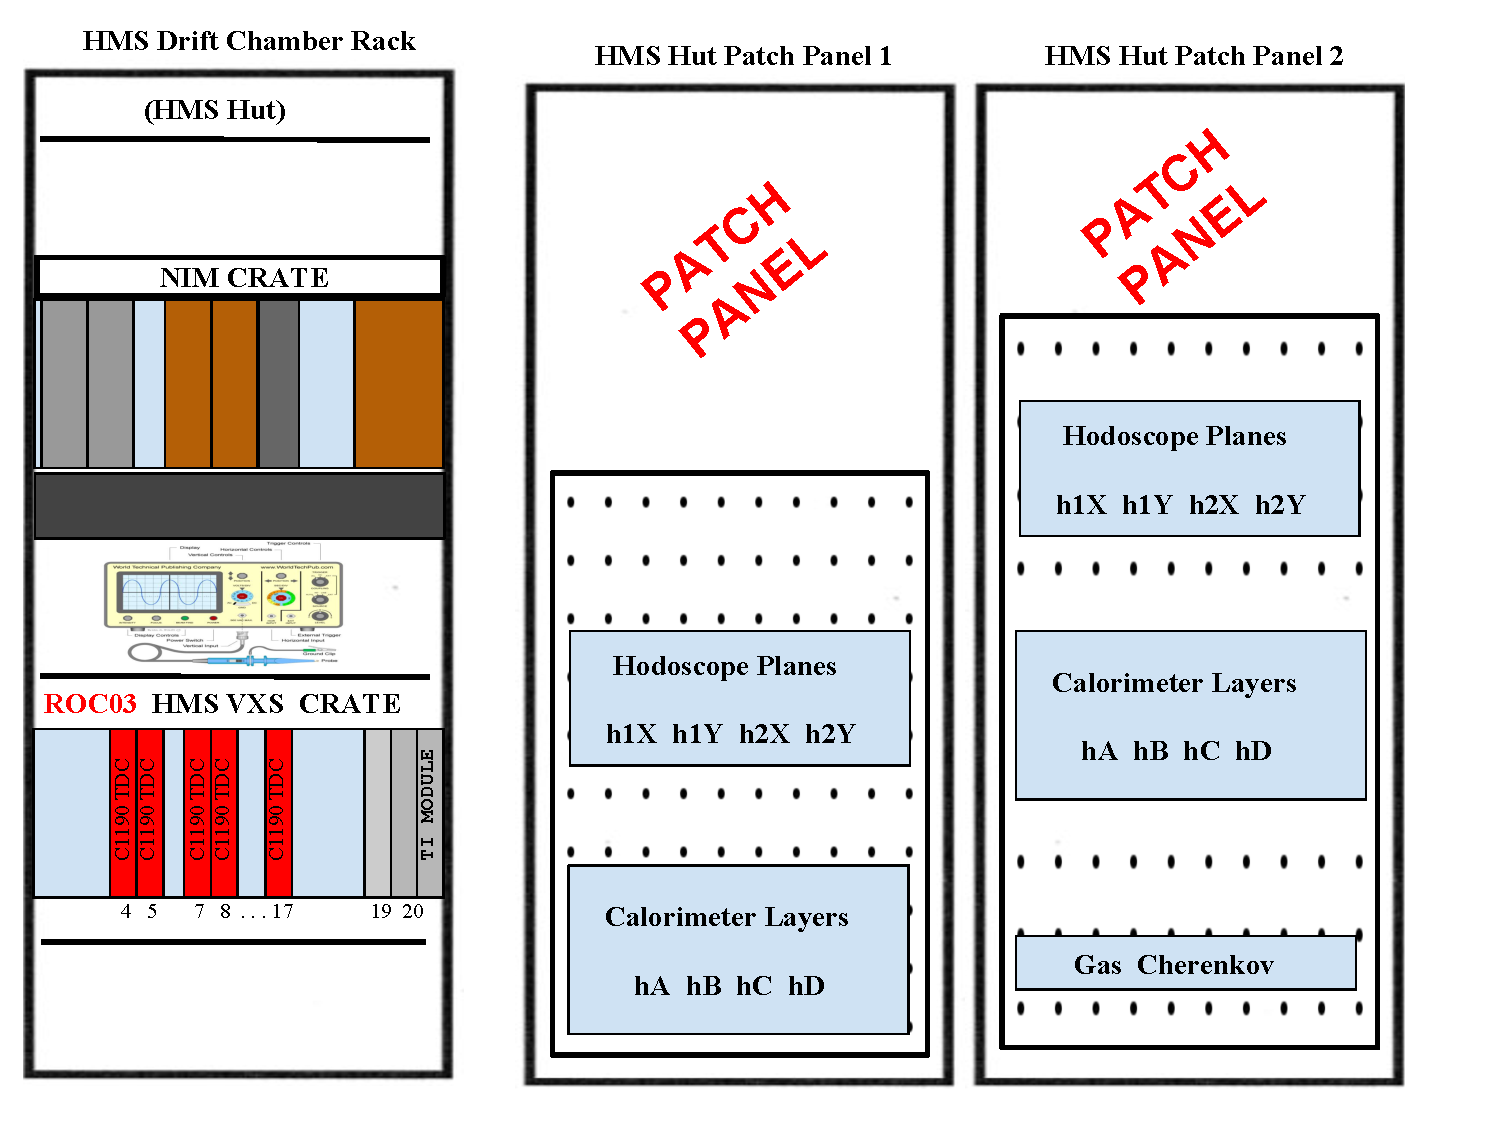
\includegraphics[width=5.0in, height=4.0in]{../HMS_Hut_Rack.pdf}
  \caption{HMS detector hut electronic rack and patch panels.}
  \label{fig:hms_hut_rack}
\end{figure}

\begin{figure}[h]
  \centering
  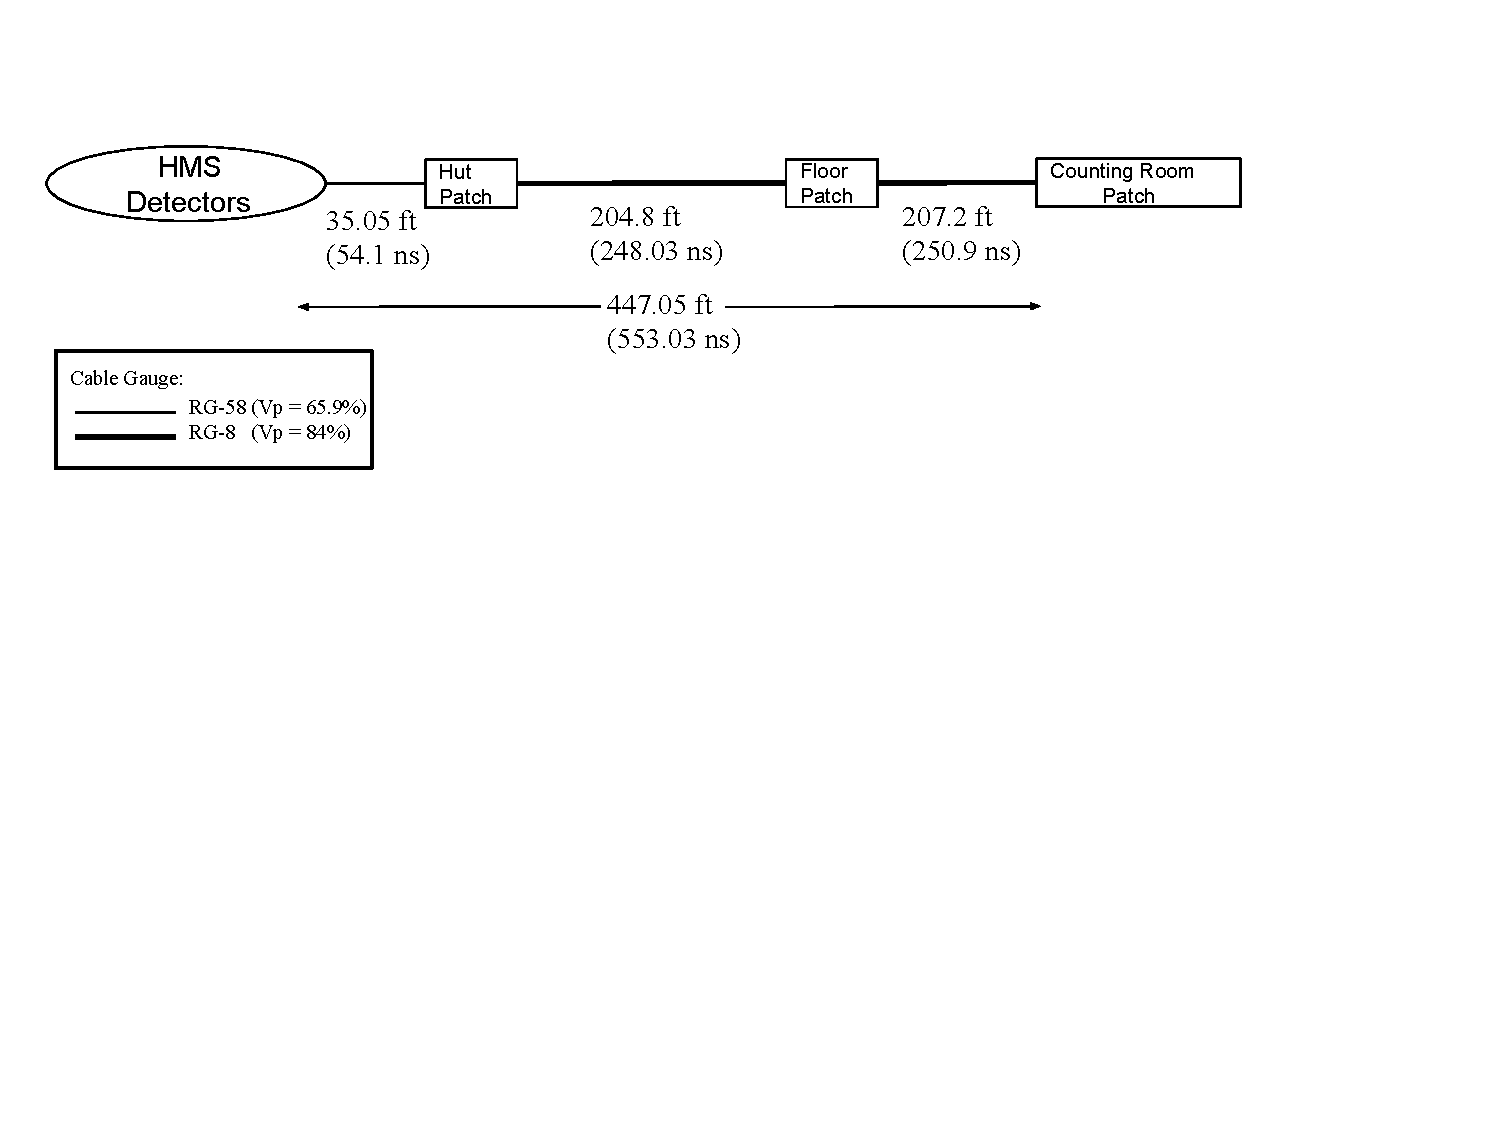
\includegraphics[width=6.0in, height=2.0in]{../HMS_patch.pdf}
  \caption{HMS Patch Diagram from detectors to Counting Room.}
  \label{fig:hms_patch}
\end{figure}

\subsection{SHMS Detector Hut}
Similarly to the HMS Drift Chambers, the SHMS Drift Chambers are also read out by TDCs in a VXS Crate in the SHMS electronics hut (See Figure \ref{fig:shms_hut_rack2}).
The Shower Counter 224 signals are fed directly into the Flash ADC (fADC-250) modules in a VXS Crate (ROC4). The Pre-Shower signals (x14/side) pass
through a 50:50 splitter and a part is fed into fADCs. The other part is partially summed in the hut and sent via the hut patch panel to the
Counting Room Patch (See Figure \ref{fig:shms_hut_rack1}). The rest of the SHMS detector signals (HGC/NGC, Hodoscope, Aerogel) are sent to the Counting Room via the hut patch panel (See Figure \ref{fig:shms_patch}). 
\newpage
\begin{figure}[h!]
  \centering
  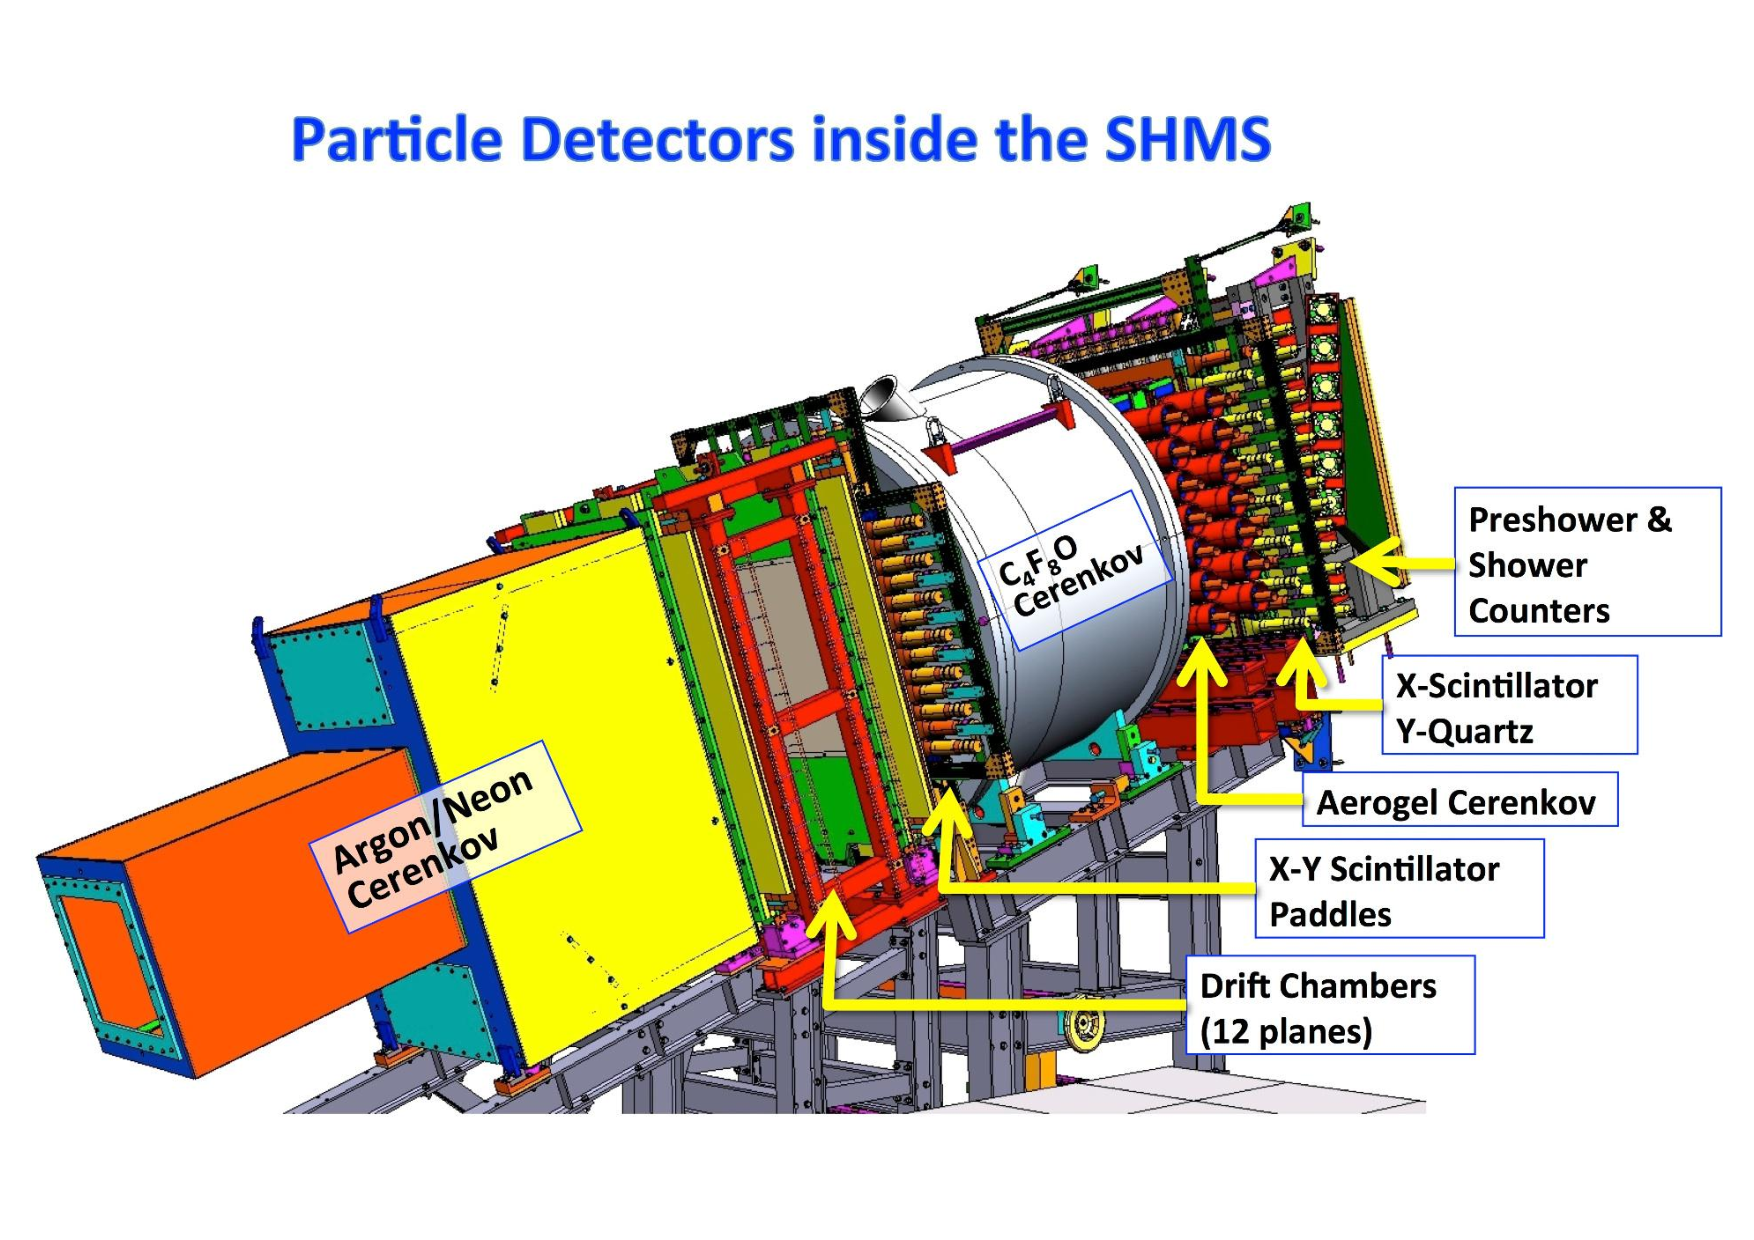
\includegraphics[width=6.0in, height=4.0in]{../SHMS_stack.pdf}
  \caption{SHMS detector stack.}
  \label{fig:shms_stack}
\end{figure}
\begin{figure}[h!]
\begin{minipage}{.5\textwidth}
  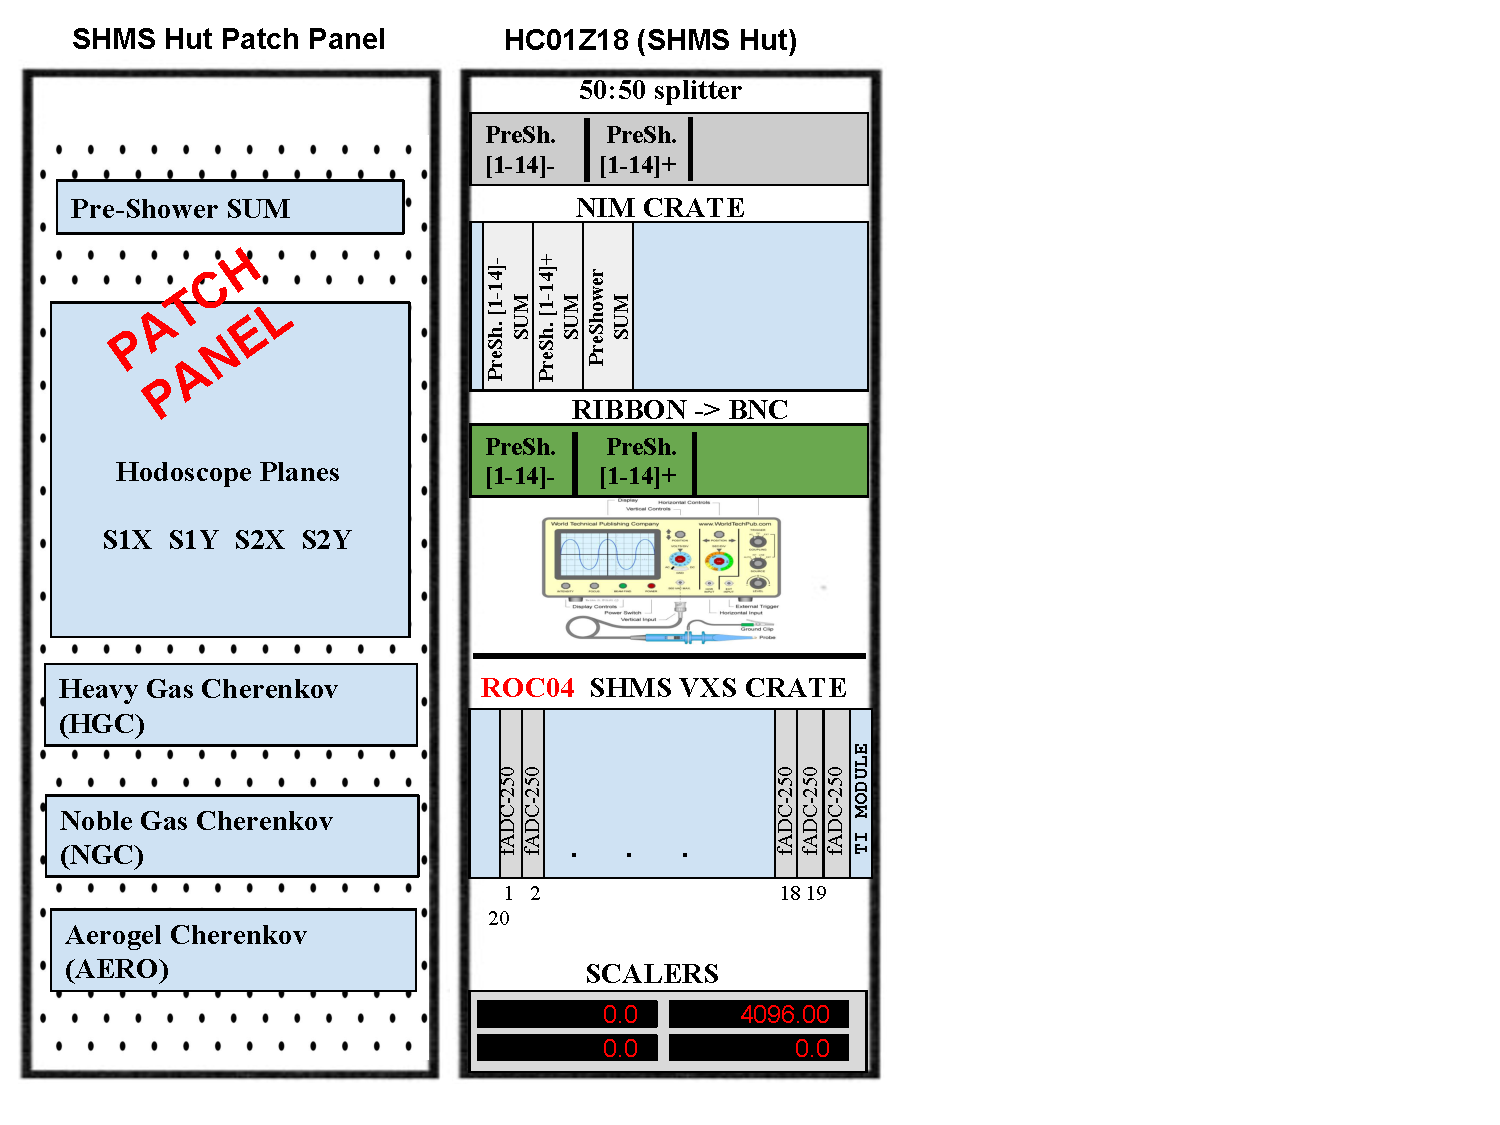
\includegraphics[width=3.0in, height=4.0in]{../SHMS_Hut_Rack01.pdf}
  \captionof{figure}{SHMS Hut Patch Panel (left) and Electronics Rack (right).}
  \label{fig:shms_hut_rack1}
\end{minipage}%
\begin{minipage}{.5\textwidth}
  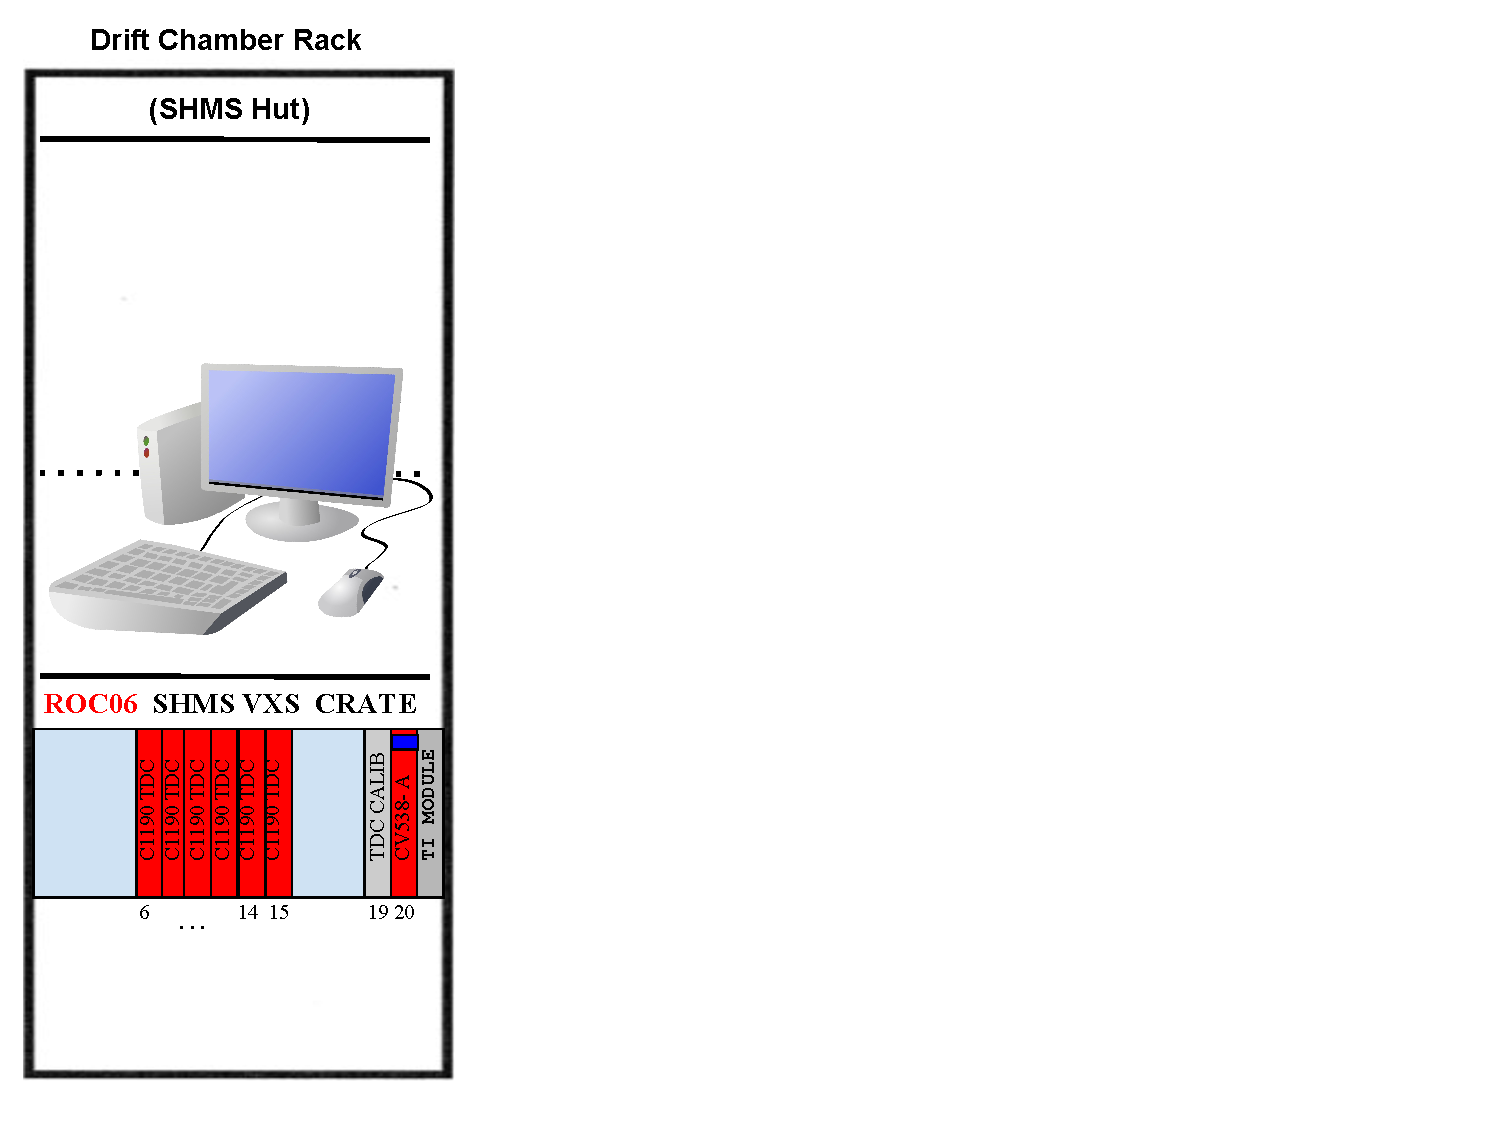
\includegraphics[width=2.0in, height=4.0in]{../SHMS_Hut_Rack02.pdf}
  \caption{SHMS Drift Chamber Electronics Rack.}
  \label{fig:shms_hut_rack2}
\end{minipage}
\end{figure}

\newpage

\begin{figure}[t]
  \centering
  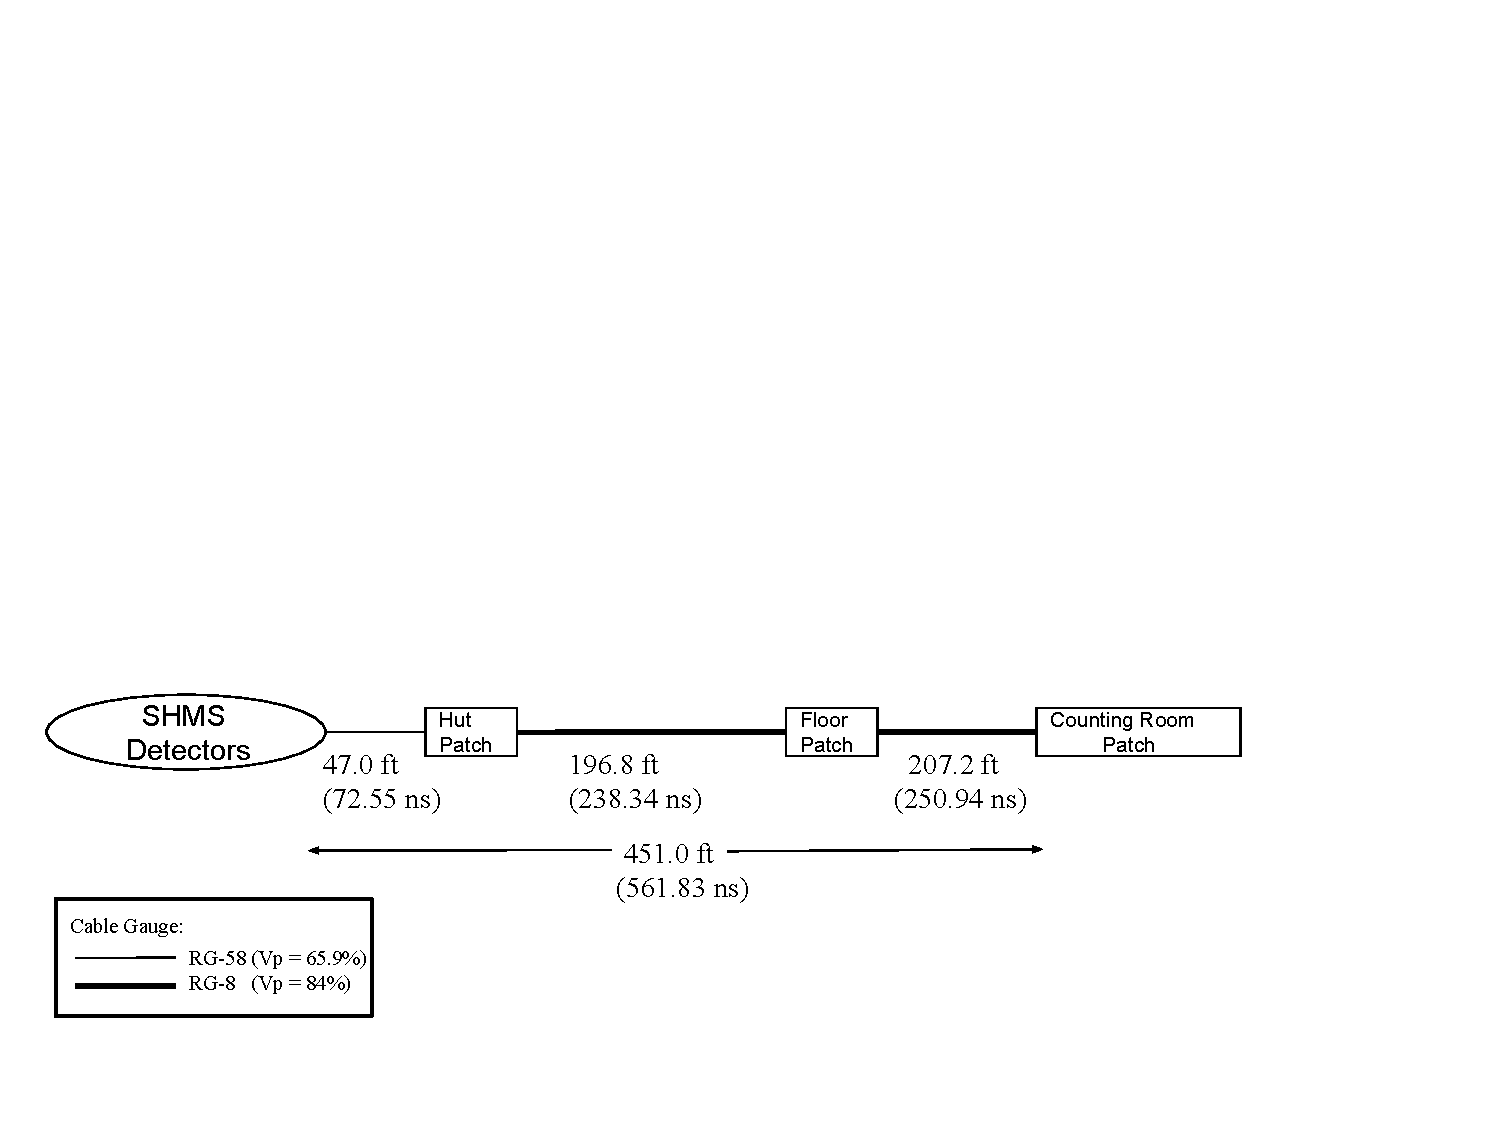
\includegraphics[scale=0.8]{../SHMS_patch.pdf}
  \caption{SHMS Patch Diagram from detectors to Counting Room.}
  \label{fig:shms_patch}
\end{figure}

\subsection{Hall C Counting Room}
Once the detector signals arrive at the Counting Room Patch (See Figure \ref{fig:cr_racks_patch}A), they are processed by the NIM/CAMAC electronics (See Figure \ref{fig:cr_racks_patch}B) to form the single arm and coincidence triggers
for each spectrometer. The signals are also sent to ADCs/TDCs to determine energy and timing information for individual detectors as well as trigger TDC information.

\begin{figure}[h!]
  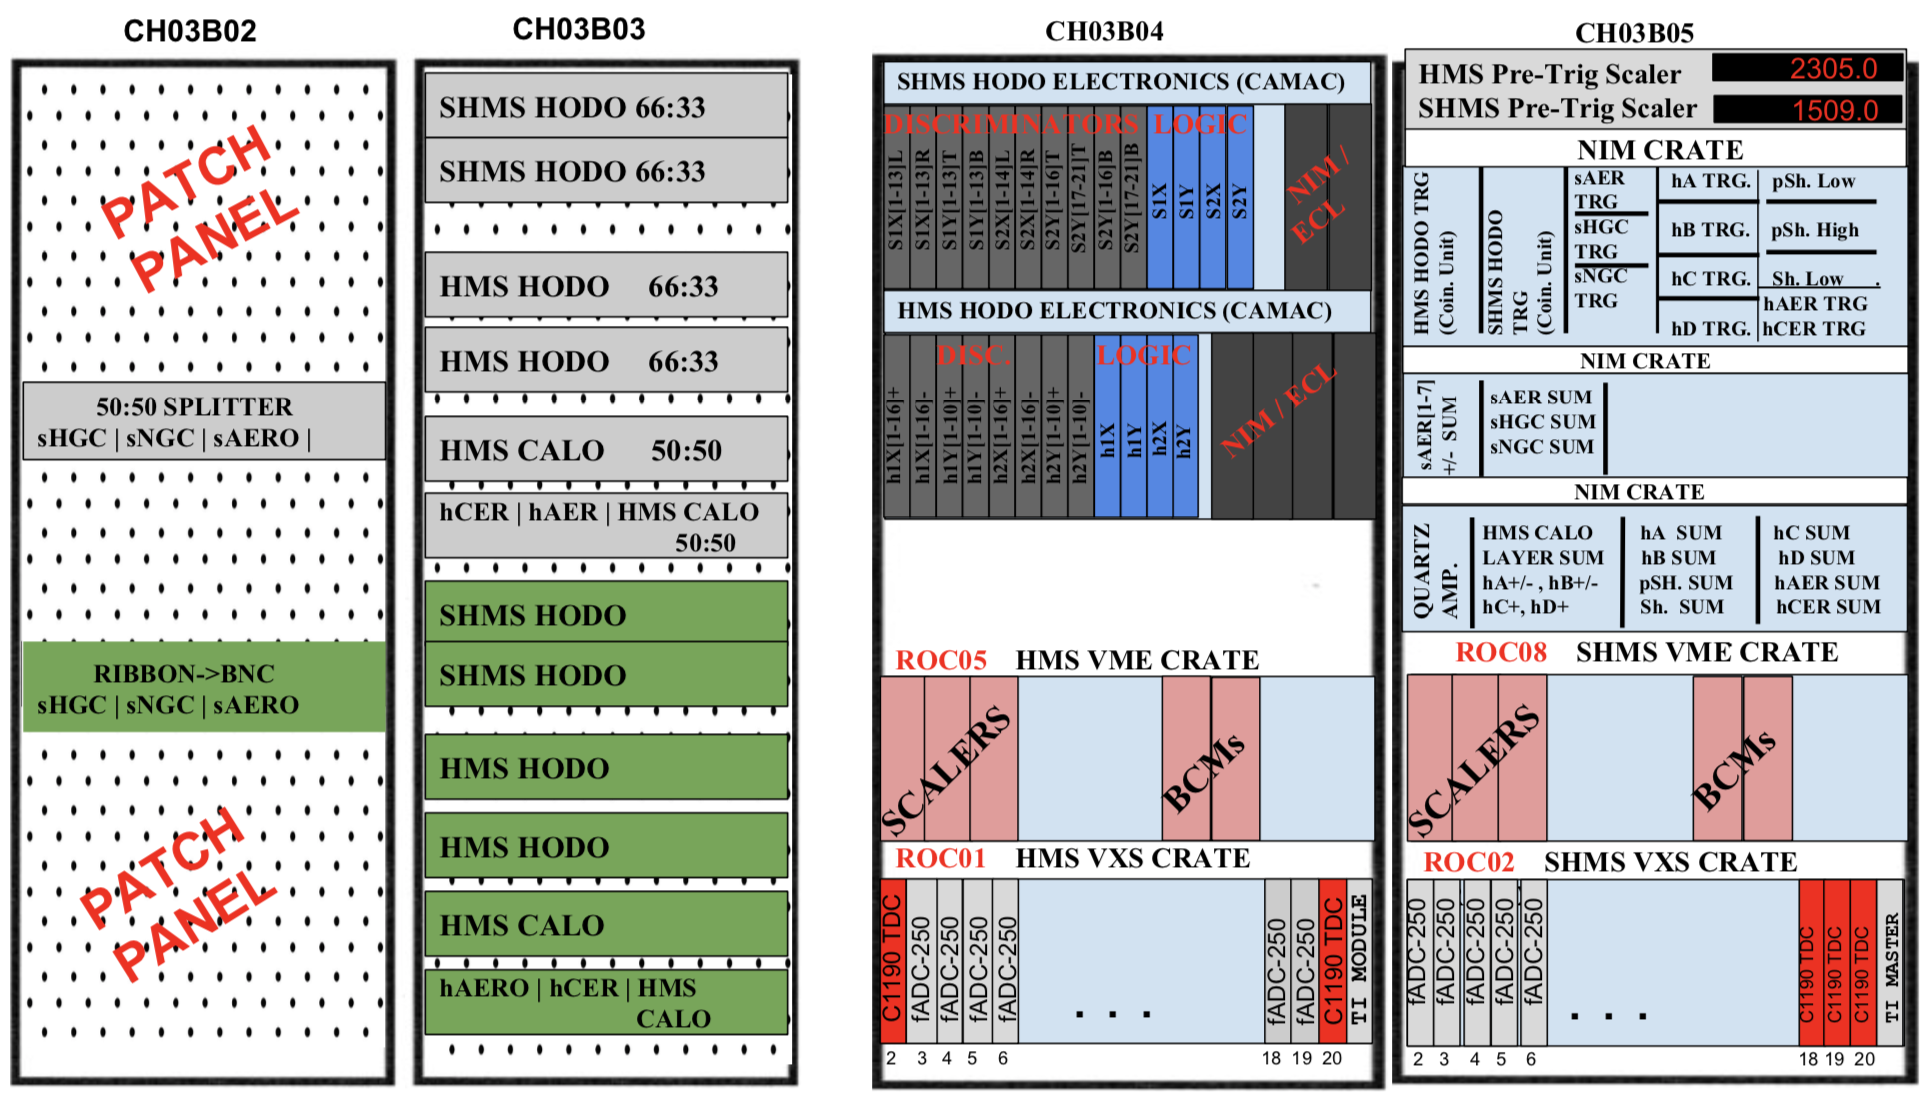
\includegraphics[scale=0.5]{../CR_patch_combined.png}
  \caption{(A) Counting Room Patch Panels (left 2 racks). (B) Counting Room main
    Electronic Racks for HMS/SHMS detectors (right 2 racks).}
  \label{fig:cr_racks_patch}
\end{figure}

\newpage
\section{HMS Trigger Set-Up} 
\indent The XY scintillator arrays (hodoscope planes) will form part of the standard HMS trigger configuration.  
Additional particle detectors may also be incorporated into the HMS trigger as required by different experiments. The Gas \v{C}erenkov and Calorimeter triggers will be
used for $e/\pi$ separation, whereas the Aerogel \v{C}erenkov trigger will be used for $\pi/K/p$ separation. 


\subsection{Hodoscope Pre-Trigger}
\begin{figure}[h!]
  \centering
  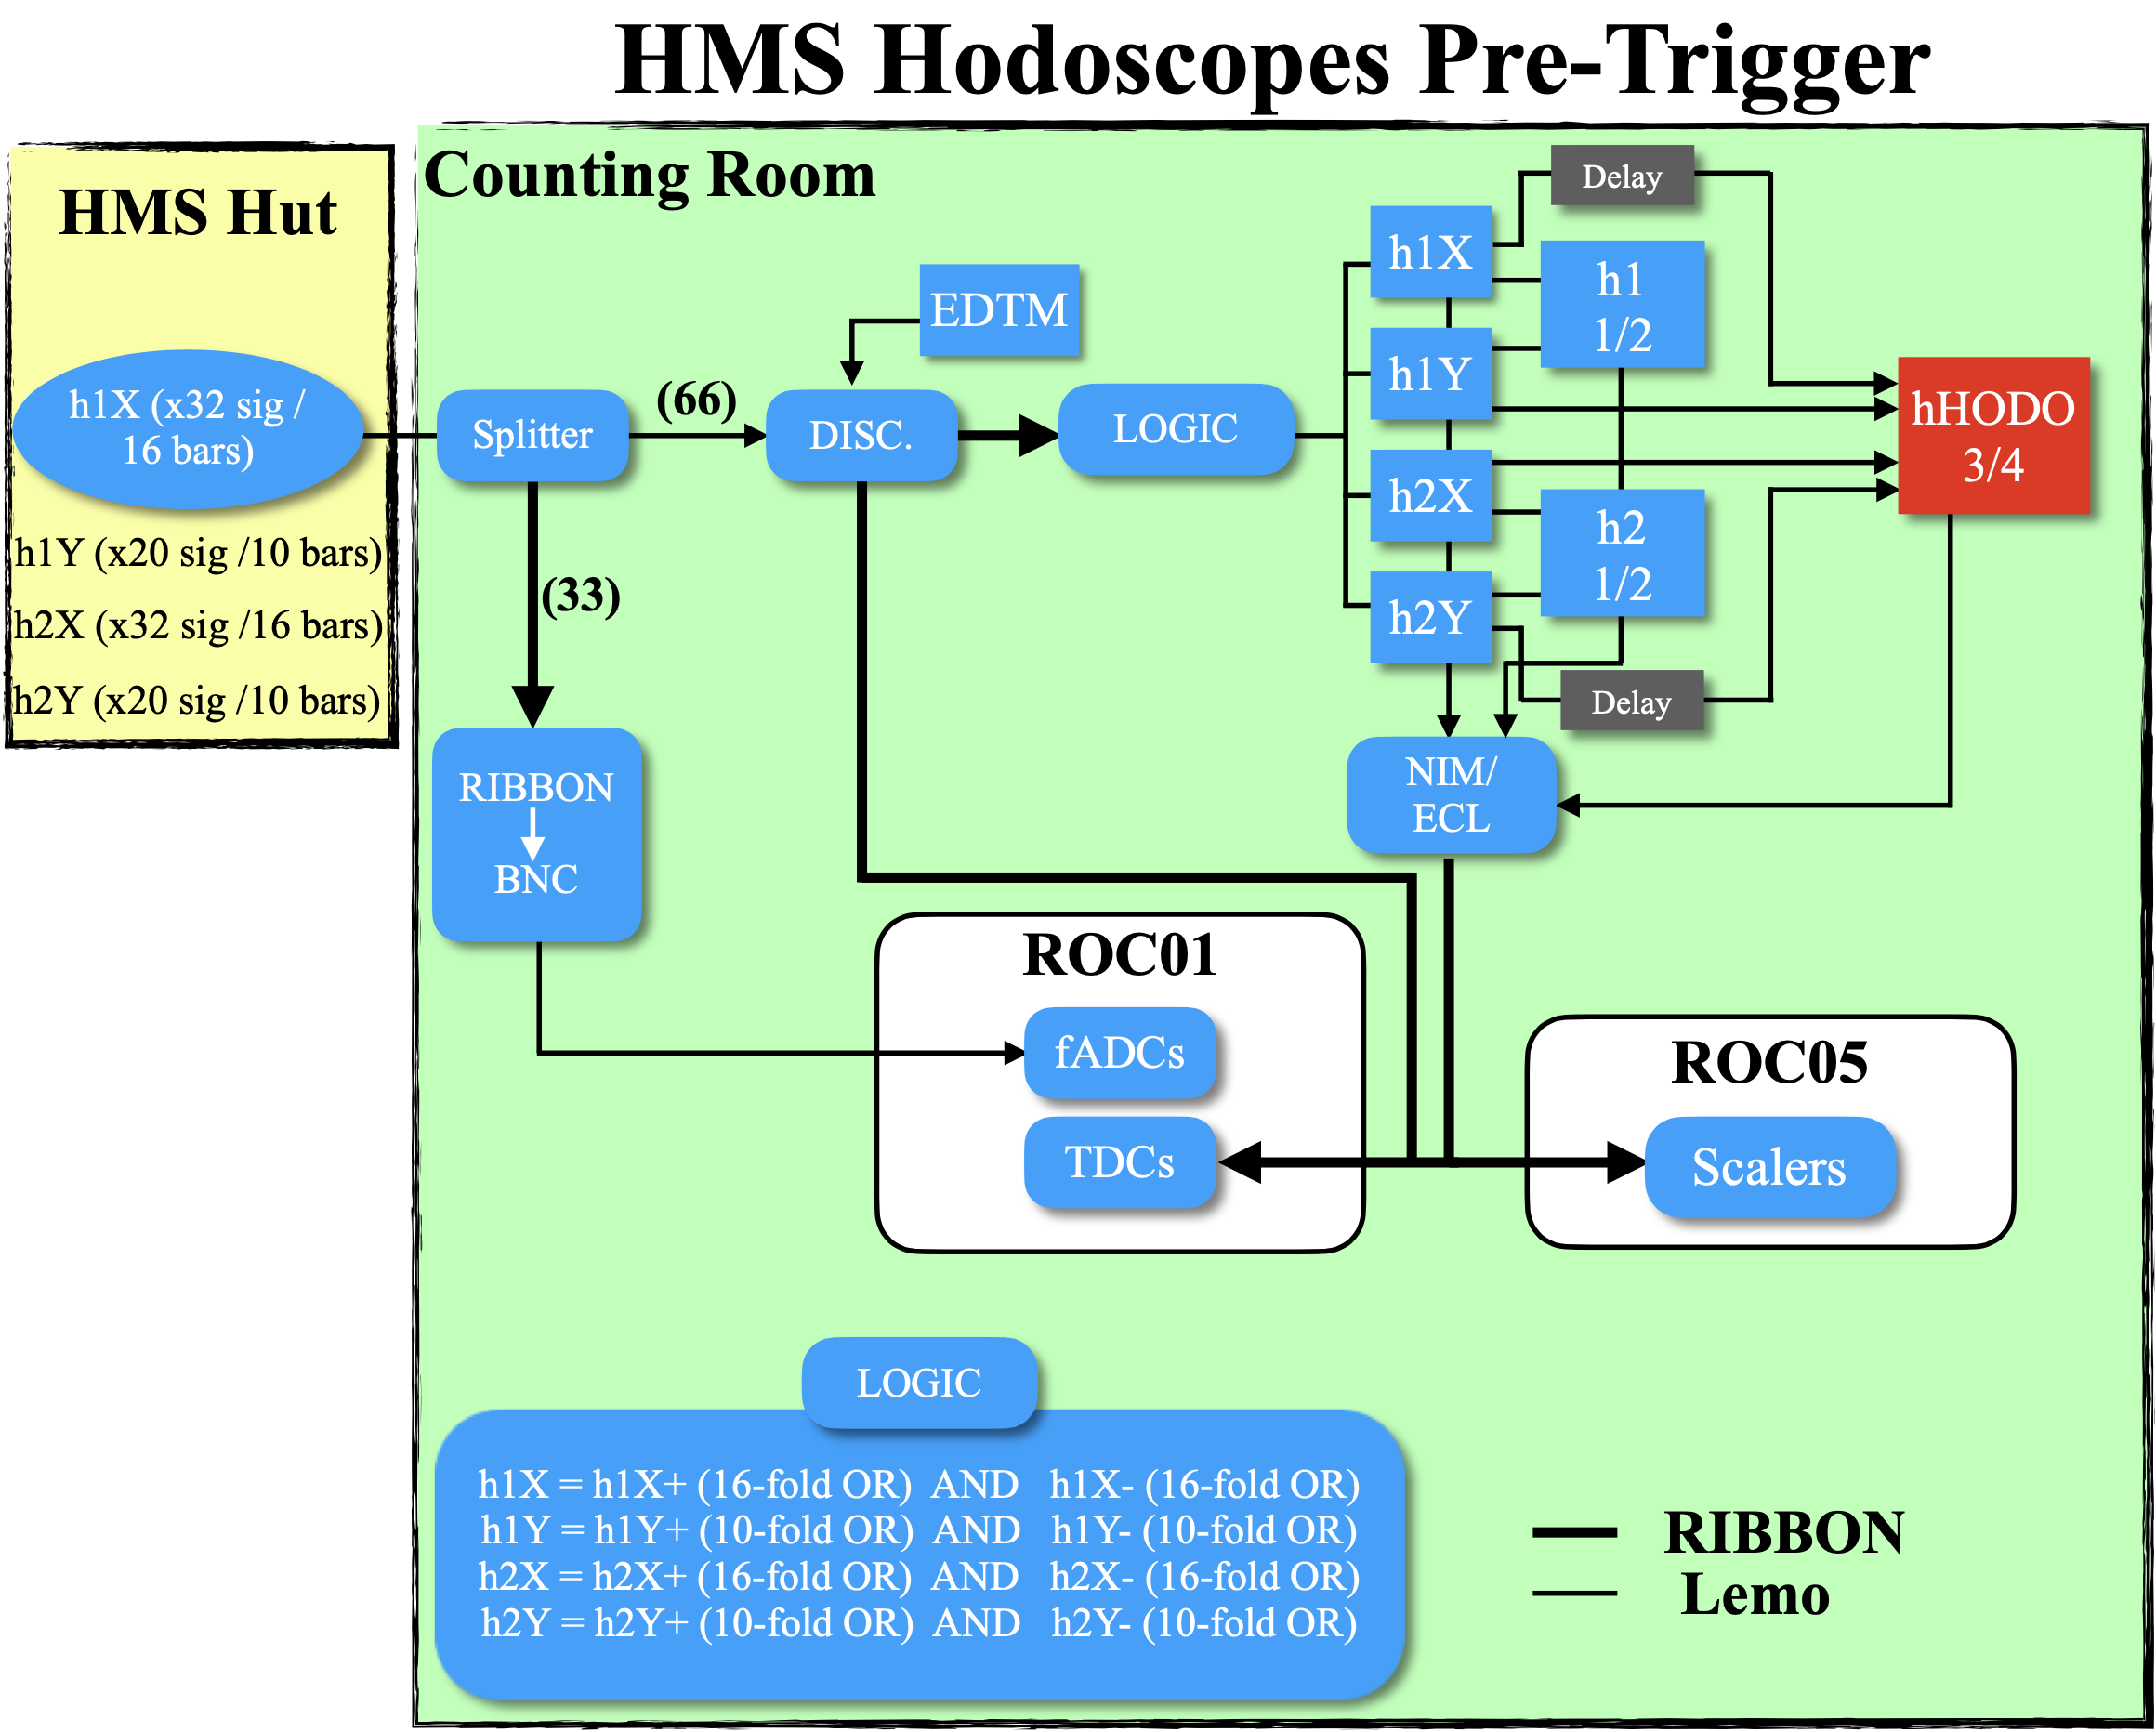
\includegraphics[scale=0.35]{./hHODO_diagram.png}
  \caption{HMS Hodoscope Electronics Diagram. For original diagram, see Appendix \ref{appendix:AppxA1}}
  \label{fig:hHODO_diagram}
\end{figure}
\noindent Each hodoscope plane consists of an array of scintillator bars coupled to a PMT at each end (See Figure \ref{fig:hms_stack}), so each bar reads out two signals. As shown in Figure \ref{fig:hHODO_diagram},
for example, hodoscope plane h1X consists of 32 signals (16 bars) read out in the Counting House (CH) patch. Each side of the plane (x16 signals/side) is fed into a 64-channel input passive splitter (16 Ch./set).
One-third (33\%) of the signal amplitude is sent via a 16-channel ribbon cable to a 64 Ch. input Ribbon-to-BNC converter (16 Ch./set) which outputs are fed into a 16-channel NIM input flash ADC (fADC). The remaining two-thirds (66\%)
of the signal amplitude is sent to a 16-Ch. input CAMAC Discriminator unit. The HMS discriminators thresholds and gate widths were set to \hhodthrs and \hhodgate, respectively.\\
\indent The discriminated signals are sent via two ribbon-cable outputs to CAEN1190 TDCs/Scalers (daisy-chained) and to a LeCroy 4564 CAMAC Logic unit to form the plane pre-triggers.
The Logic Unit takes four sets of 16-Ch. input ribbon cable and forms a 16-fold OR for each set by default. Further boolean operations are done through the module backplane by connecting a twisted pair cable to the pin corresponding to the
desired boolean operation. For hodoscope plane pre-triggers, the boolean operations are as follows:
\begin{empheq}[box=\fbox]{align*}
& \text{h1X = h1X+ (16-fold OR) \textit{AND} h1X- (16-fold OR)} \\ 
& \text{h1Y = h1Y+ (10-fold OR) \textit{AND} h1Y- (10-fold OR)} \\
& \text{h2X = h2X+ (16-fold OR) \textit{AND} h2X- (16-fold OR)} \\ 
& \text{h2Y = h2Y+ (10-fold OR) \textit{AND} h2Y- (10-fold OR)} 
\end{empheq}

\indent Once a pre-trigger has been made for each plane, they are sent to a NIM/ECL converter (Level Translator - Phillips Scientific (or P/S) Model 7126) via twisted pair cables to convert the ECL signal (twisted pair)
to a NIM signal. The NIM output is then sent to individual sets of a P/S Model 752 NIM Logic unit to adjust the widths of each of the plane pre-triggers as necessary before making a coincidence. An X-Y hodoscope plane
coincidence (h1 = h1X \textit{AND} h1Y, h2 = h2X \textit{AND} h2Y) is then made by feeding each hodoscope X-Y plane pair into a P/S Model 755 Nim Logic unit. A copy of each of the four individual plane pre-triggers is also sent to another set of P/S Model 755 to make a 3/4 or
4/4 plane coincidence (via a front-panel knob) which defines the production hodoscope pre-trigger. A copy of all the pre-triggers discussed above are sent to TDCs/Scalers via a NIM/ECL converter for timing and counting rate information. (See Figure \ref{fig:hHODO_diagram}) \\


\subsection{Calorimeter Pre-Trigger}
\begin{figure}[h!]
  \centering
  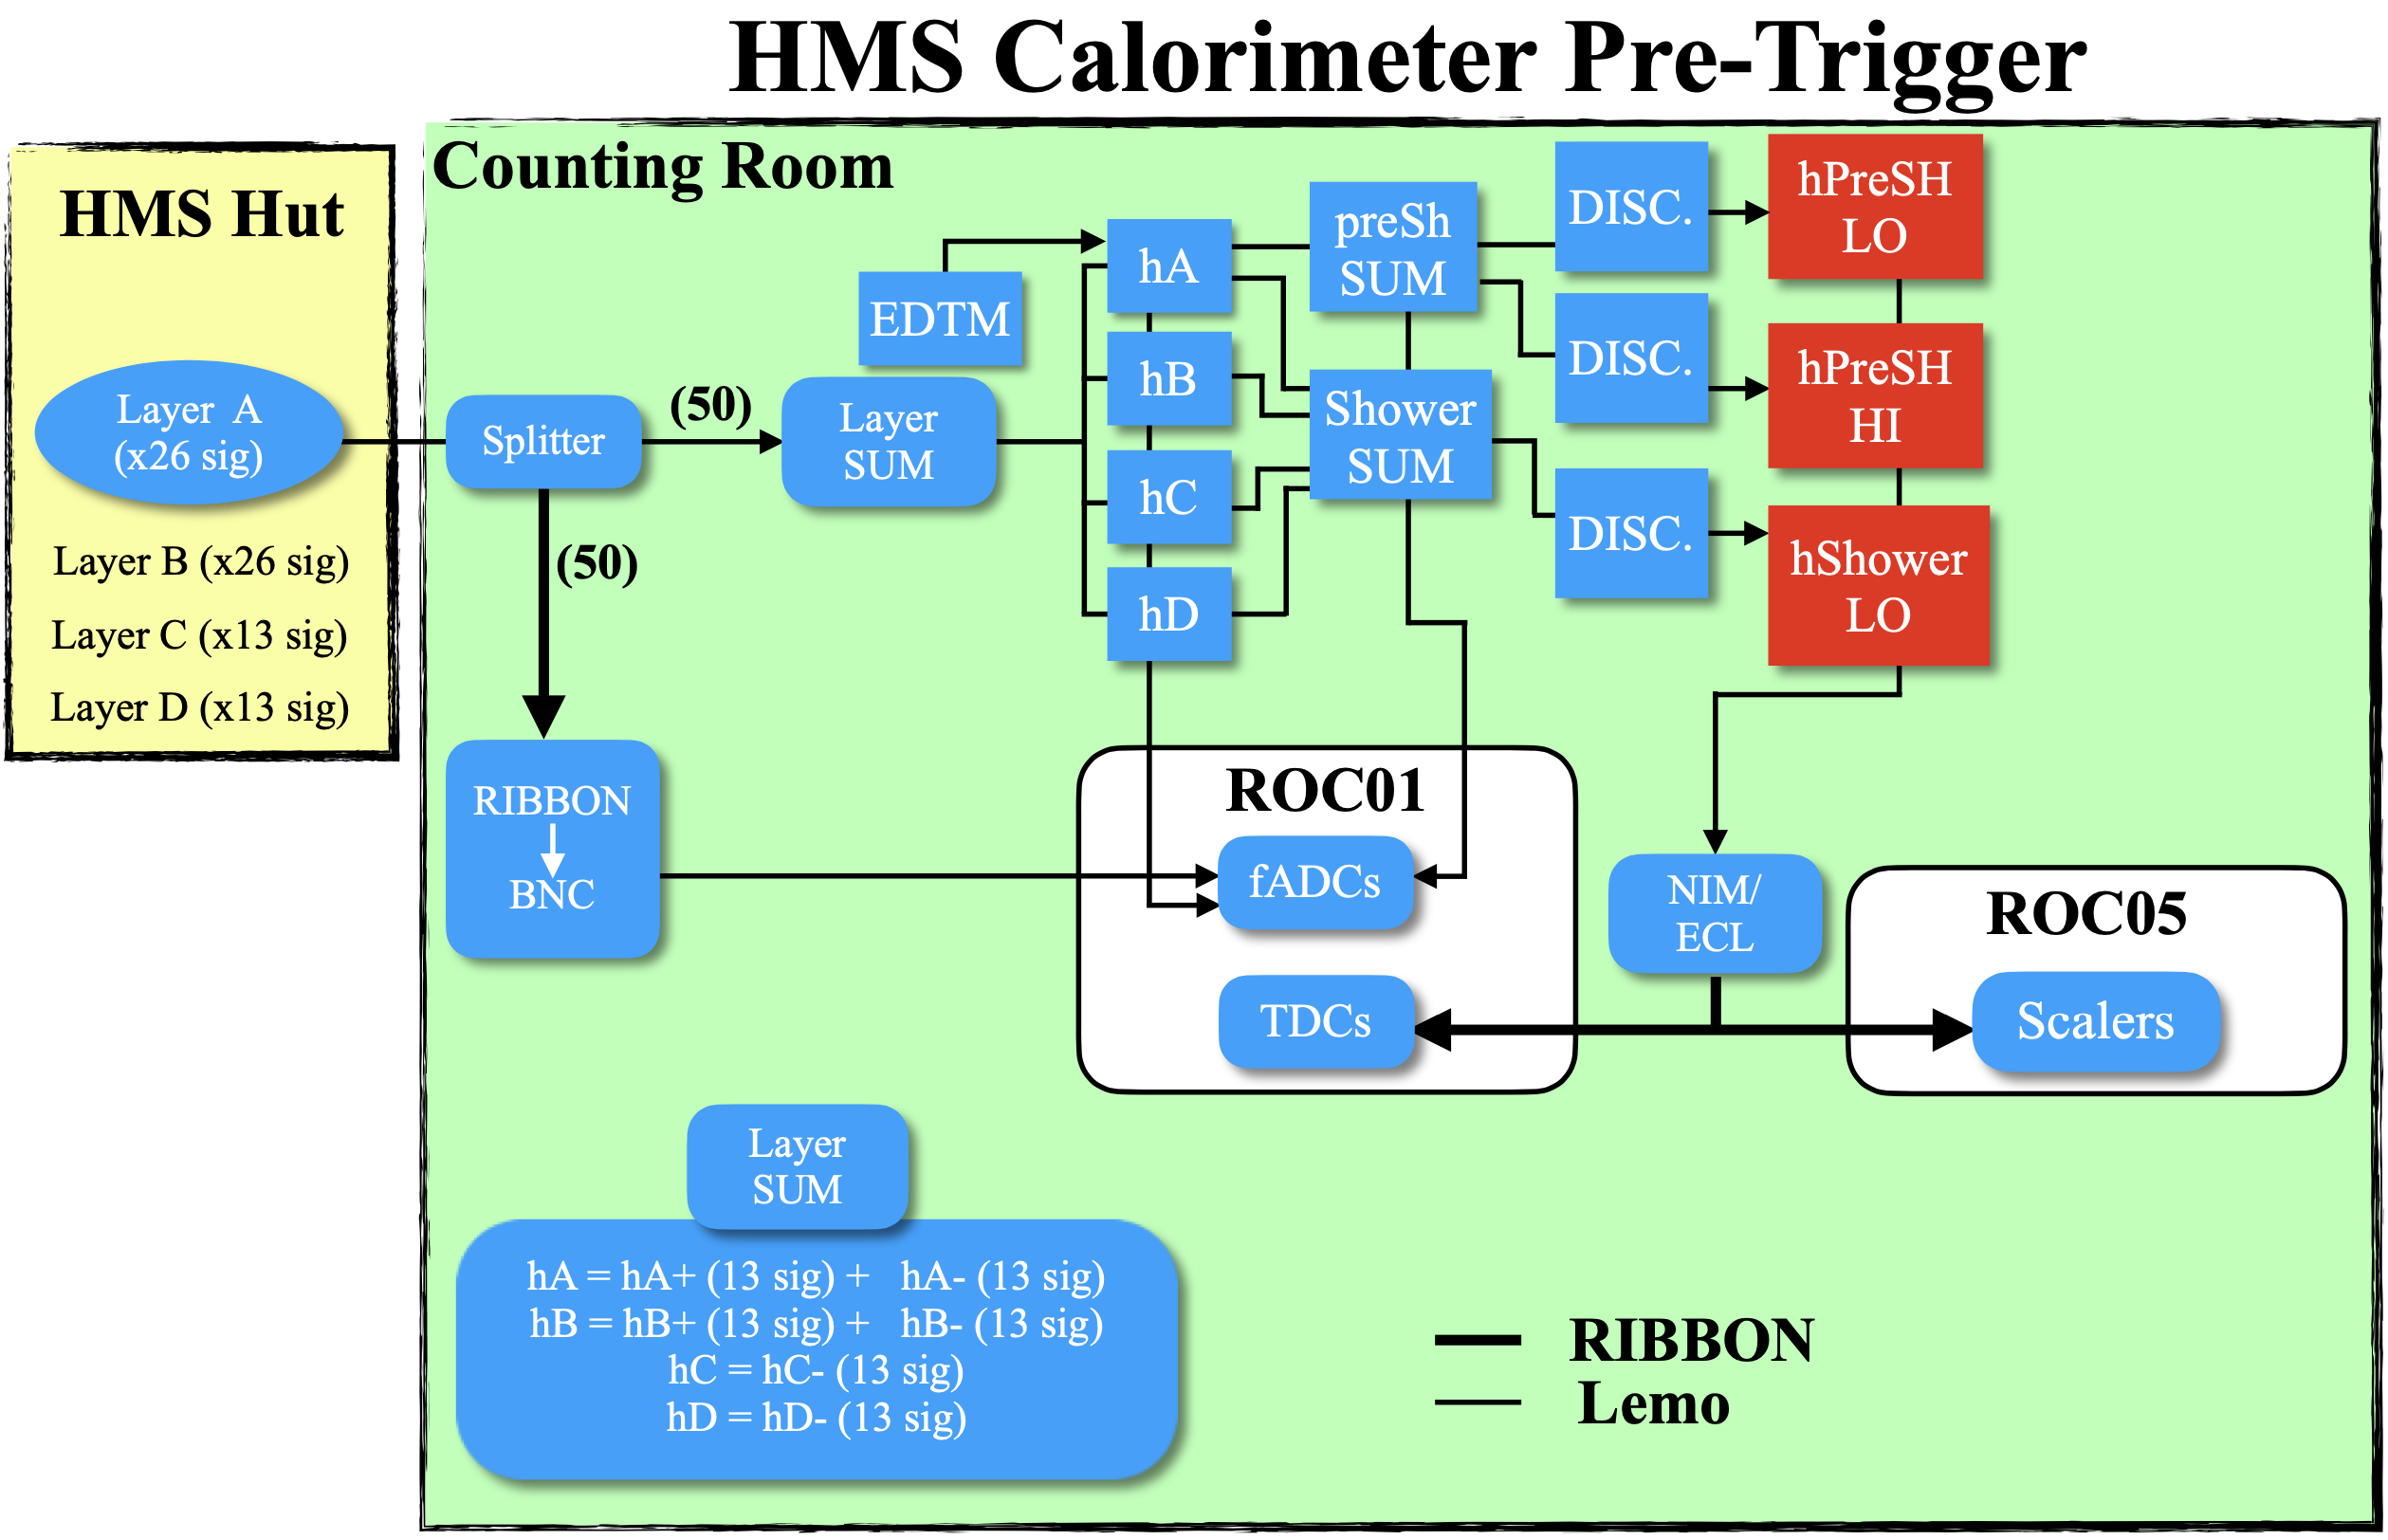
\includegraphics[scale=0.35]{./hCAL_diagram.png}
  \caption{HMS Calorimeter Electronics Diagram. For original diagram, see Appendix \ref{appendix:AppxA2}}
  \label{fig:hCAL_diagram}
\end{figure}
\noindent The HMS Calorimeter consists of four layers of lead blocks. Layers A and B read out a 26 PMT signals per layer (13 signals/side) while layers C and D
read out 13 signals/layer on one side. The first layer form the Pre-Shower counter while all four layers (A, B, C and D) form the Shower counter.  
Each layer is read out in the Counting Room patch and fed into 50:50 splitters. One output of the splitter is fed to fADCs via a Ribbon-to-BNC converter (same as hodoscopes)
while the other output is sent to a P/S Model 740 NIM Linear FI/FO summing modules. Each side of a layer is summed first (hA+, hA-, hB+, hB-, hC and hD sums). The sums are fed into
a LeCroy Model 428F summing module where layers hA+/- and hB+/- are summed to form hA and hB sums. A copy of each layer sum is sent to fADCs. The Pre-Shower SUM is then made from the sum of layer A, while the Shower SUM is made by summing all four layers. A copy of the Pre-Shower and Shower sums is also sent to fADCs. The Pre-Shower and Shower sums are then sent to a P/S Model 715
NIM Discriminator unit to form the PreShower Low/High (LO/HI) and Shower Low pre-triggers with thresholds \hPrShLo, \hPrShHi and \hSHLo, respectively with all gate widths set to 30 ns. A copy of the pre-triggers is sent to TDCs/Scaler modules for trigger timing and counting rate
information.

\subsection{Gas \v{C}erenkov Pre-Trigger} \label{hms_cer_section}
\begin{figure}[h!]
  \centering
  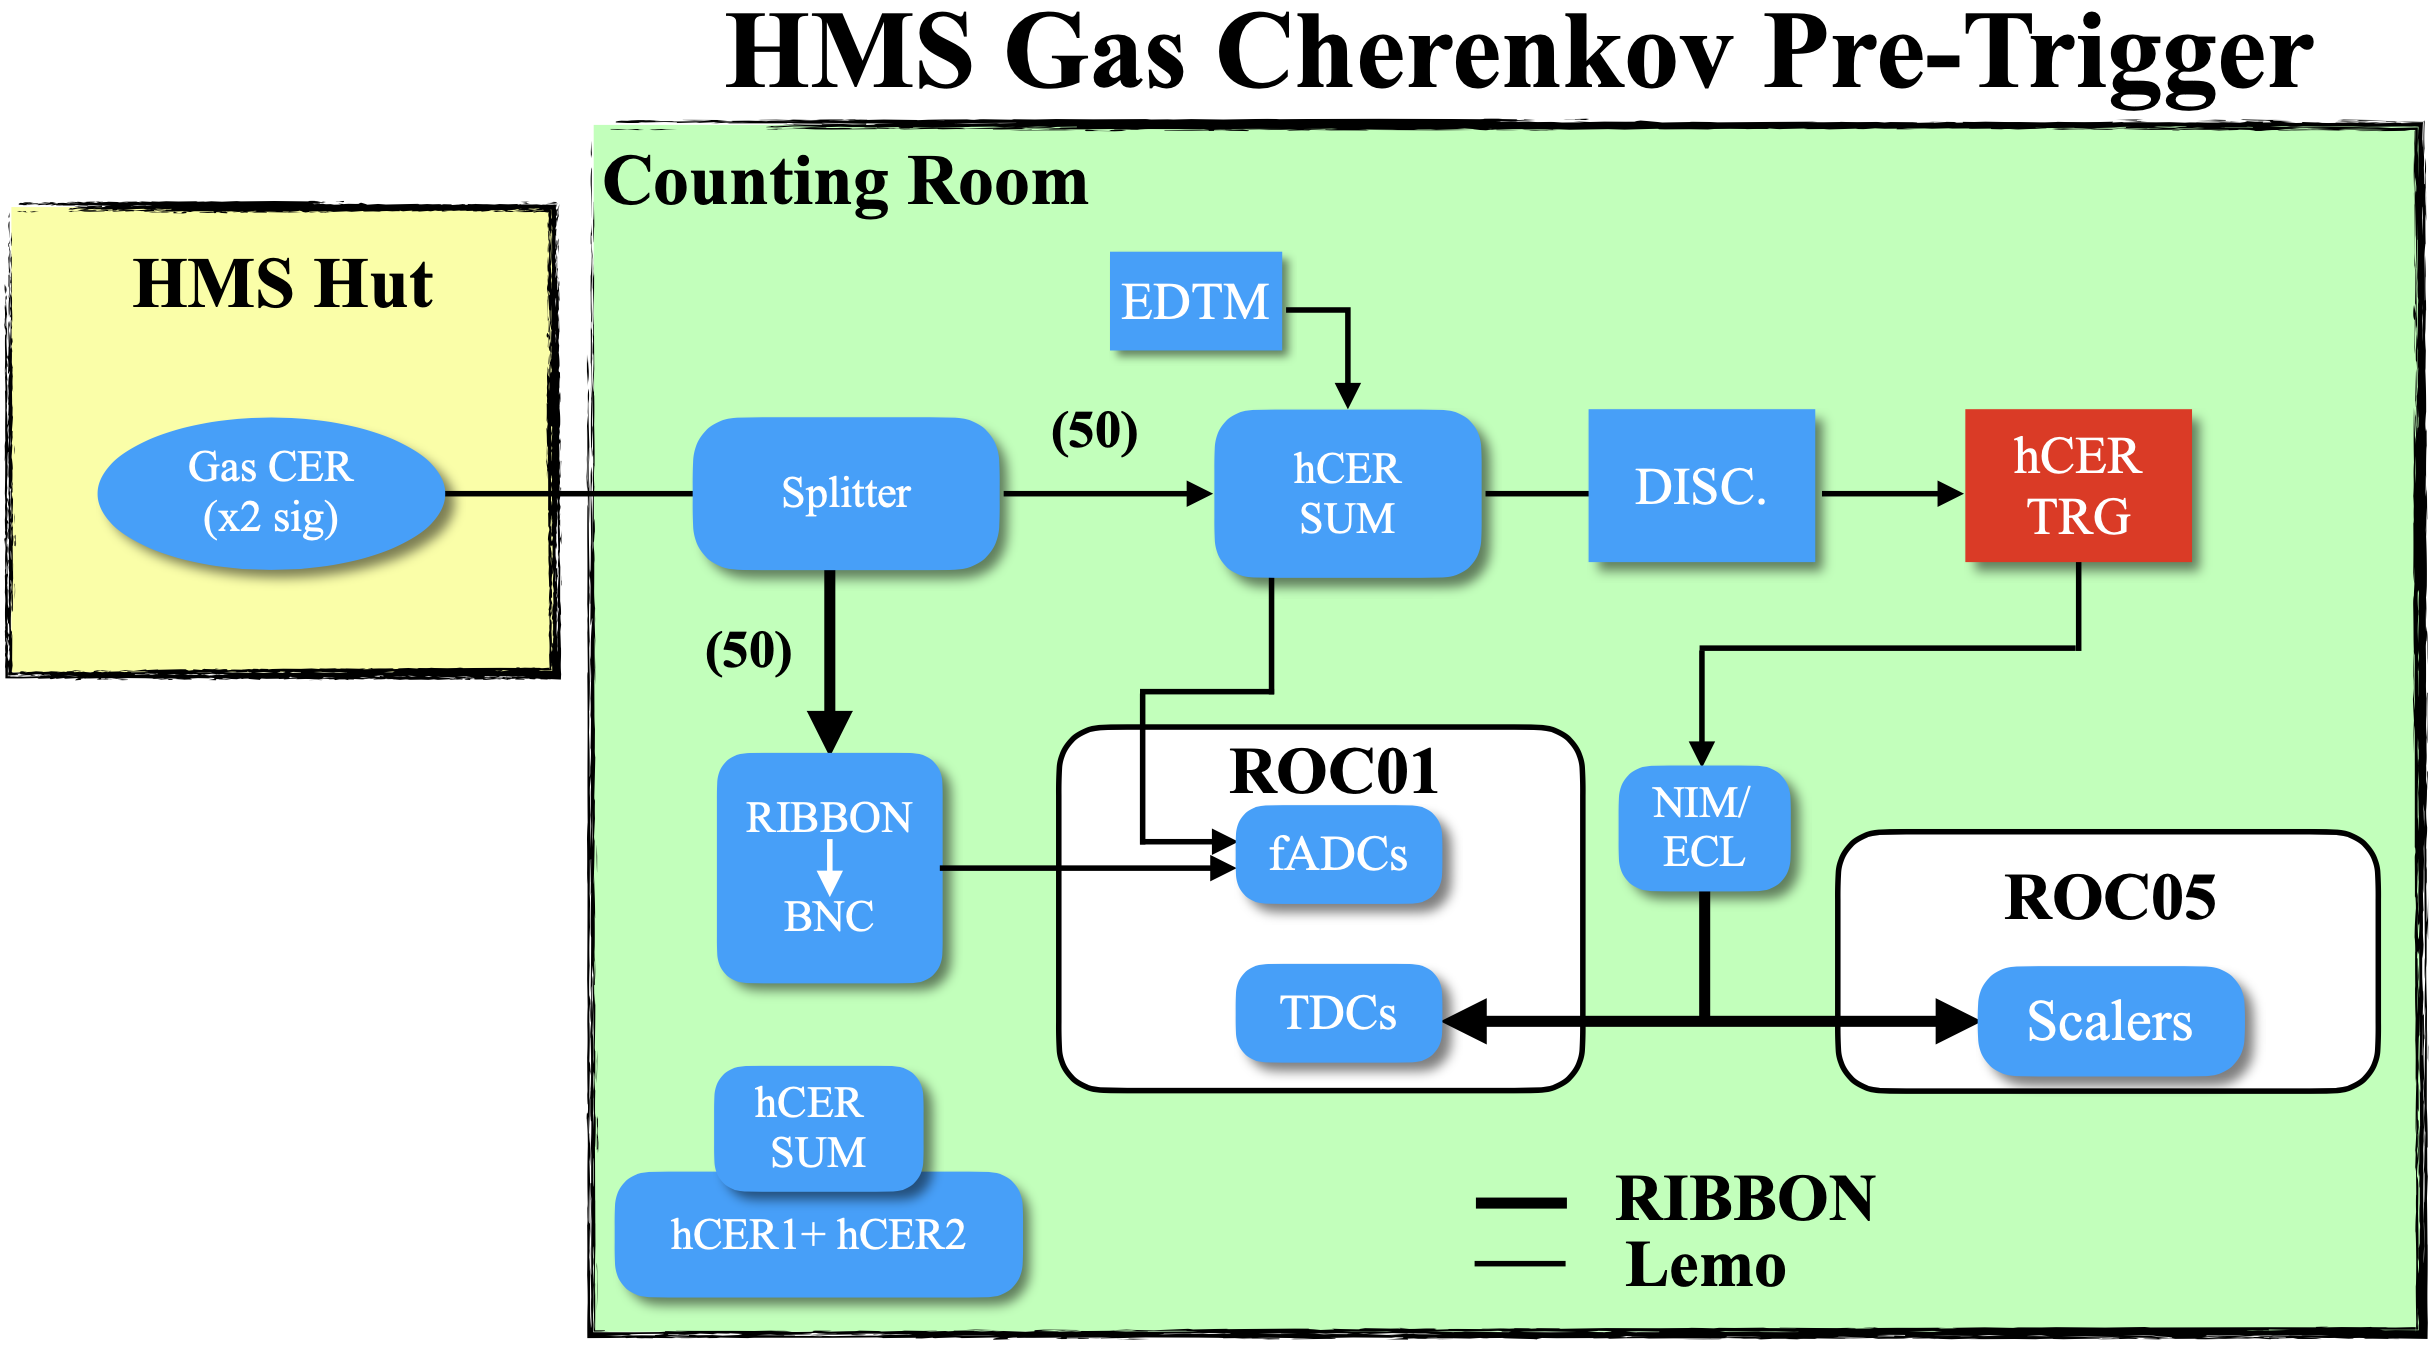
\includegraphics[scale=0.35]{./hCER_diagram.png}
  \caption{HMS Gas \v{C}erenkov Electronics Diagram. Same electronics diagram applies for SHMS Gas \v{C}erenkov. For original diagram, see Appendix \ref{appendix:Appx3} }
  \label{fig:hCER_diagram}
\end{figure}

\indent The HMS Gas \v{C}erenkov detector consists of a 1.5 m long cylindrical tank between the first and second set of hodoscope planes (See Figure \ref{fig:hms_stack}).
The tank is filled with a gas and has two spherical mirrors that focus the \v{C}erenkov photons towards two 5-inch PMTs\cite{hms_cer_article}. The
signals are read out in the Counting Room patch and pass through a 50:50 splitter. One output is fed into
an fADC module via a Ribbon-to-BNC converter. The other output is sent to a LeCroy Model 428F summing module, and a copy of the sum is fed to an fADC. The sum is
also sent to a P/S Model 715 NIM discriminator to form the \v{C}erenkov pre-trigger with a threshold and gate width set to \hcerthrs and \hcergate. A copy of the discriminated signal is also sent to TDCs/Scalers via a NIM/ECL converter for trigger and counting rate information.


\subsection{Aerogel \v{C}erenkov Pre-Trigger}

\indent The HMS Aerogel \v{C}erenkov detector consists of a 120cm x 70cm rectangular aerogel tray coupled to a diffusion box\cite{hms_aero_article} and is located
between the second Drift Chamber and first set of hodoscope planes. The diffusion box has 8 PMTs on each side
which detect \v{C}erenkov light produced by interactions with the Aerogel material. The signals are sent directly to the Hall C Floor Patch Panel, and then
read out in the Counting Room patch and pass through a 50:50 splitter. One output is fed into an fADC module via a Ribbon-to-BNC converter. The other output is
sent to a summing module, and a copy of the sum is fed to an fADC. The sum is also sent to a NIM discriminator to form the Aerogel pre-trigger.
A copy of the discriminated signal is also sent to TDCs/Scalers via a NIM/ECL converter for trigger and counting rate information.
The electronics diagram is the same as in Figure \ref{fig:hCER_diagram}. For the original diagram, see Appendix \ref{appendix:Appx4}

\newpage
\subsection{HMS Single Arm Pre-Trigger}\label{ssec:hms_single_arm_sec}
\begin{figure}[h!]
  \centering
  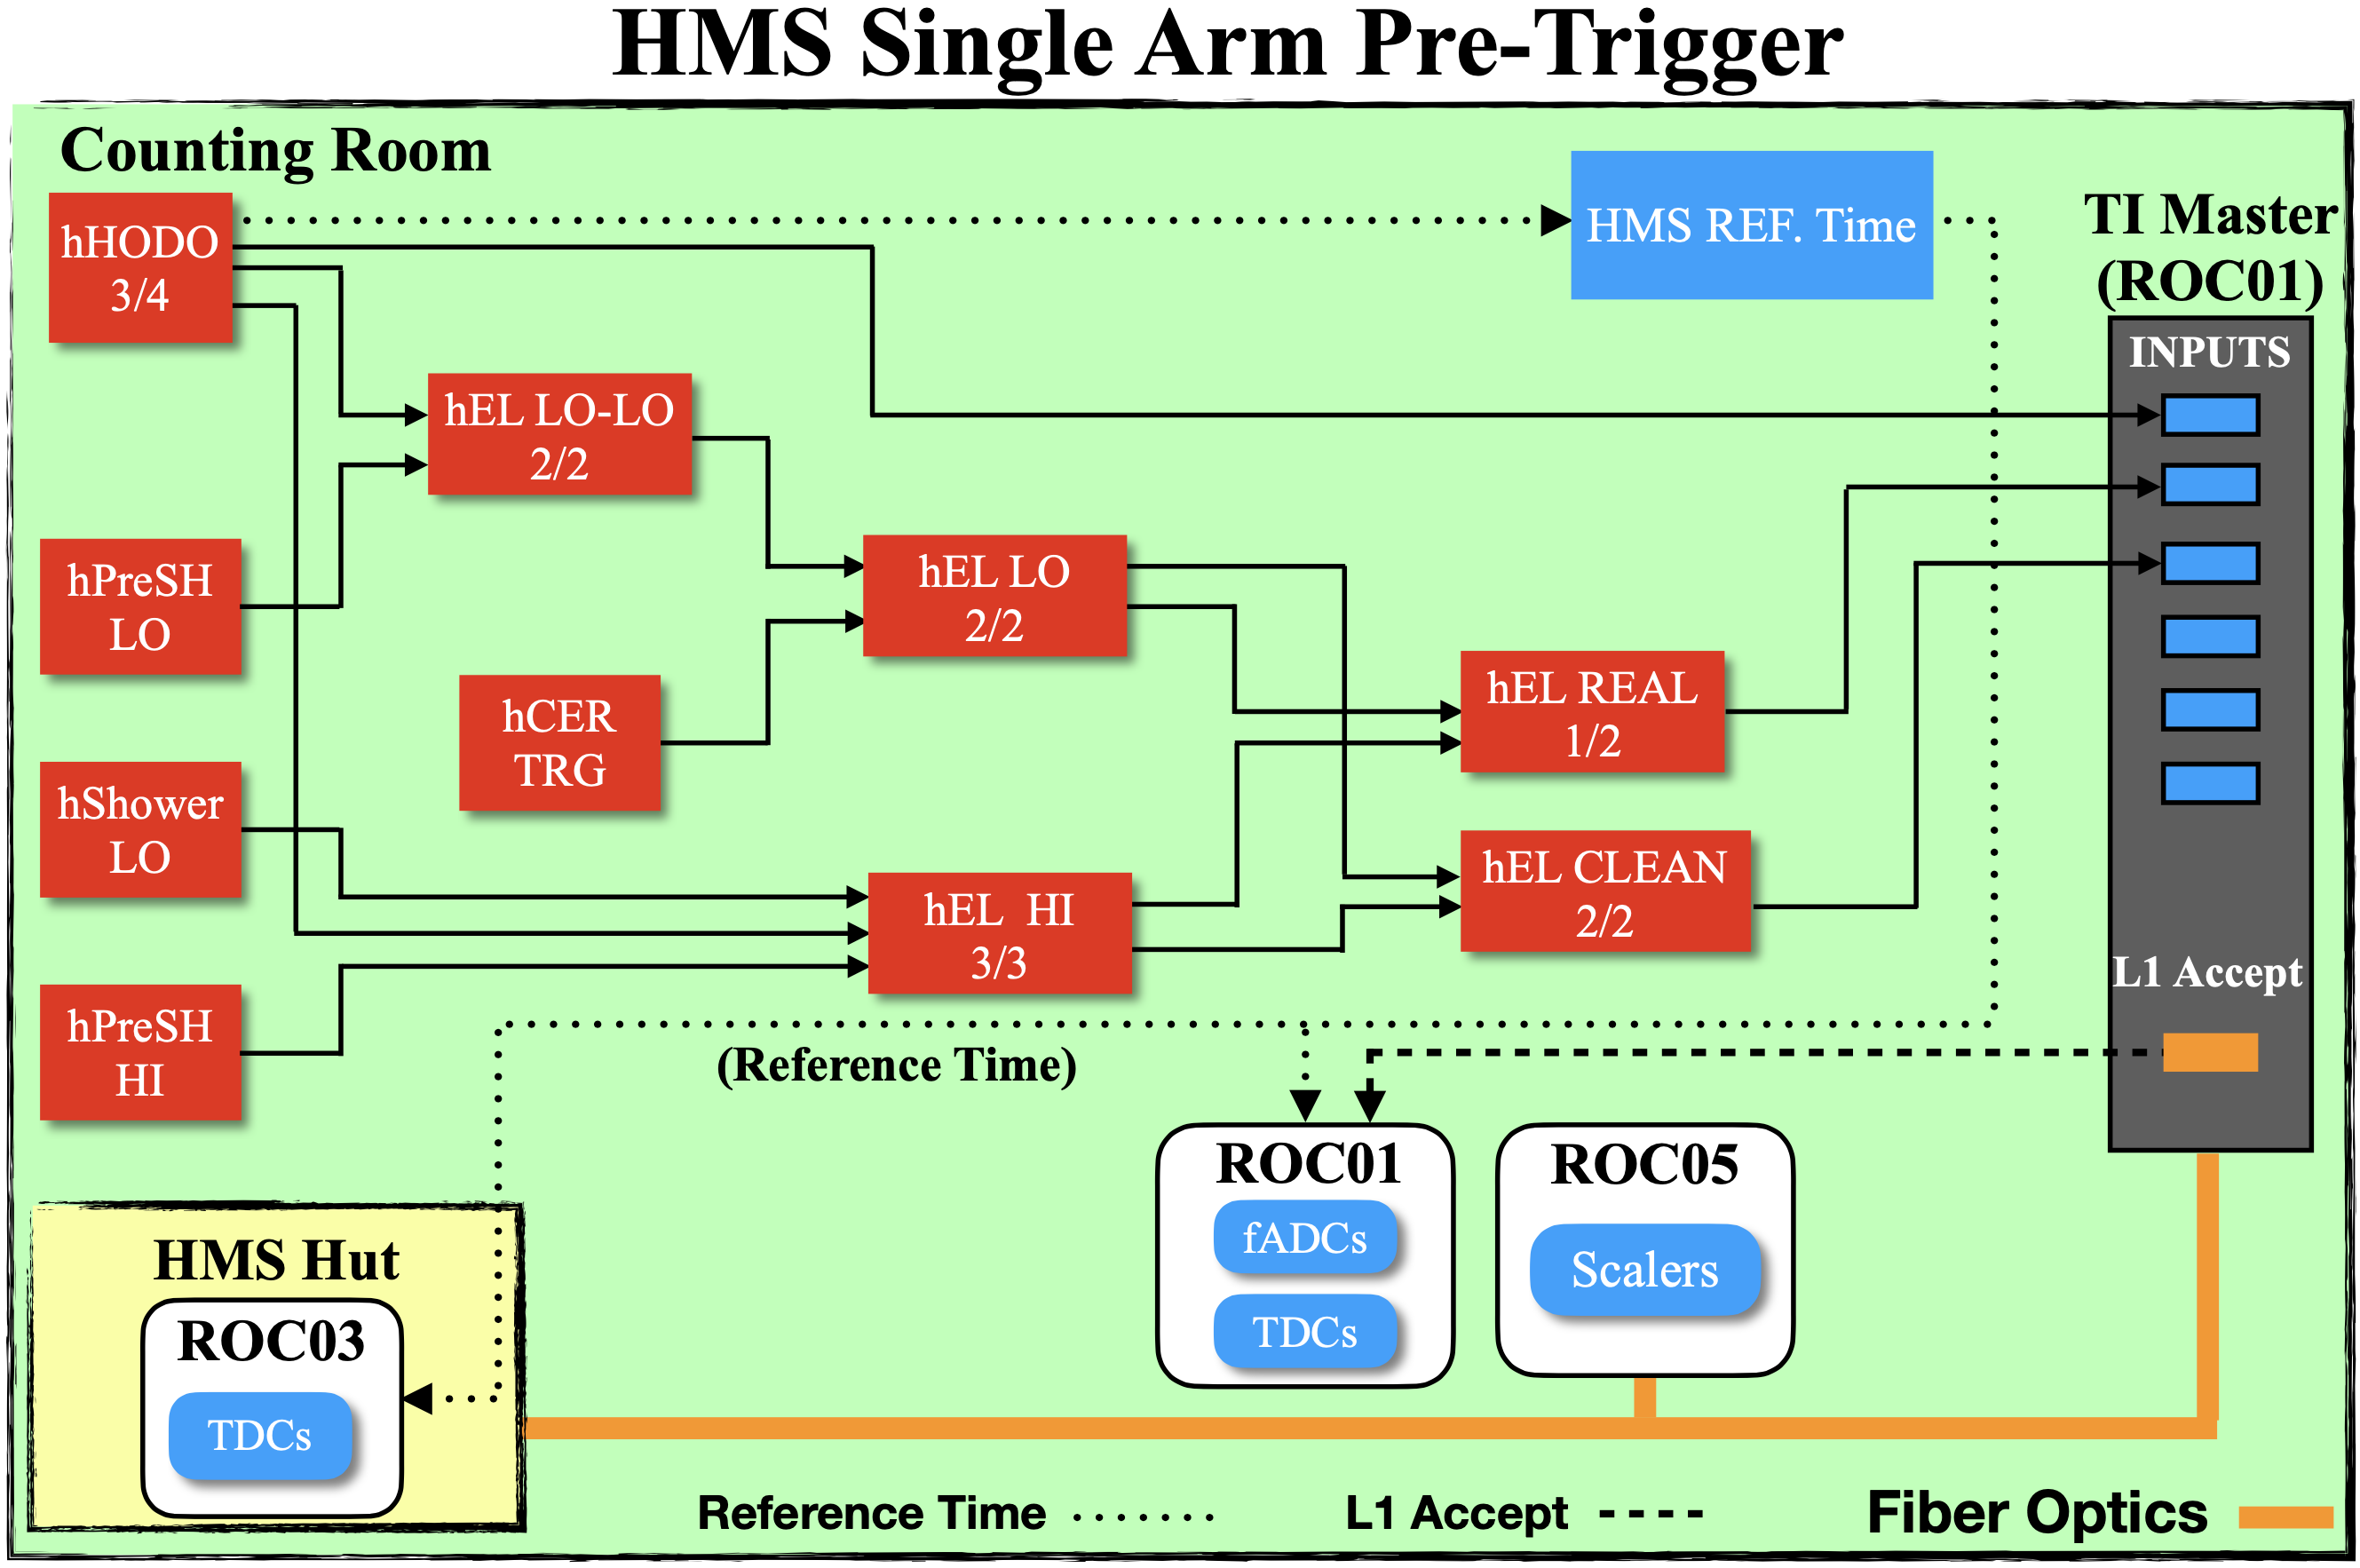
\includegraphics[scale=0.35]{HMS_SingleArm_diagram.png}
  \caption{HMS Single Arm Pre-Trigger Electronics Diagram. For original diagram, see Appendix \ref{appendix:Appx5}}
  \label{fig:HMS_SingleArm_diagram}
\end{figure}

\indent The HMS single arm pre-trigger will be formed from the standard pre-trigger (hodoscopes) and a combination of other detector pre-triggers as required by the
experiment. The standard and other \textit{experiment-specific} pre-triggers are sent to a P/S  Model 755 NIM Logic unit to form a single-arm coincidence.
Once the HMS pre-trigger is formed, a copy is sent to Scalers/TDCs. The other copy is sent to a NIM/ECL converter, where three copies of the HMS pre-trigger are sent
via ECL twisted pairs to two CAEN 1190 TDC modules and an input on the TI\footnote{In single-arm mode, the TI in ROC 01 is known as \textit{TM or Trigger Master}, and its main operation is to distribute a copy
of the accepted triggers to all ROCs related to the HMS via fiber optic lines. The same applies to the SHMS when operated in single-arm mode.} known as the \textit{Trigger Supervisor or TS} (up to six trigger inputs). The copies sent to
the TDCs are fed externally through the 16th pin of a 16-channel input ribbon cable adaptor\footnote{Each TDC module in the readout crate (ROC 01) must receive a copy of the HMS pre-trigger known as
the \textit{reference time} via twisted pairs. The reference time in each TDC module functions as a common stop for all detector signals being fed to the TDC.} The pre-trigger
copy sent to the Trigger Supervisor is processed, accepted and disseminated throgh the crate backplane to all modules (except TDCs) in the crate. The TDCs are NOT configured to not receive a copy
of the accepted triggers, therefore, a copy must be sent from the ``TRG'' ECL output in TI front panel to the TDC ``TRG'' NIM input\footnote{A copy of the accepted triggers is needed by ADCs/TDCs in order to initiate
readout in all channels of the respective modules.} via a NIM/ECL converter. The inputs are daisy-chained
with other TDCs present in the crate. A copy of the accepted triggers is also sent to Scalers/TDCs.

\newpage 
\section{SHMS Trigger Set-Up}
\indent The three planes (X1, Y1, X2) of scintillator arrays and the Quartz plane (Y2) will form part of the standard SHMS trigger configuration (See Figure \ref{fig:shms_stack}).  
Additional particle detectors may also be incorporated into the SHMS trigger as required by different experiments. The Noble Gas \v{C}erenkov \footnote{Noble Gas \v{C}er: e/$\pi$ separation $\geq$ 6 GeV/c} and
Calorimeter triggers will be used for e/$\pi$ separation, whereas the Heavy Gas\footnote{Heavy Gas \v{C}er: $\pi$/K separation above 3.4 GeV/c} and Aerogel \v{C}erenkov trigger will be used for $\pi$/K/p
separation\cite{SHMS_PID}. 

\subsection{Hodoscopes Pre-Trigger}
\begin{figure}[h!]
  \centering
  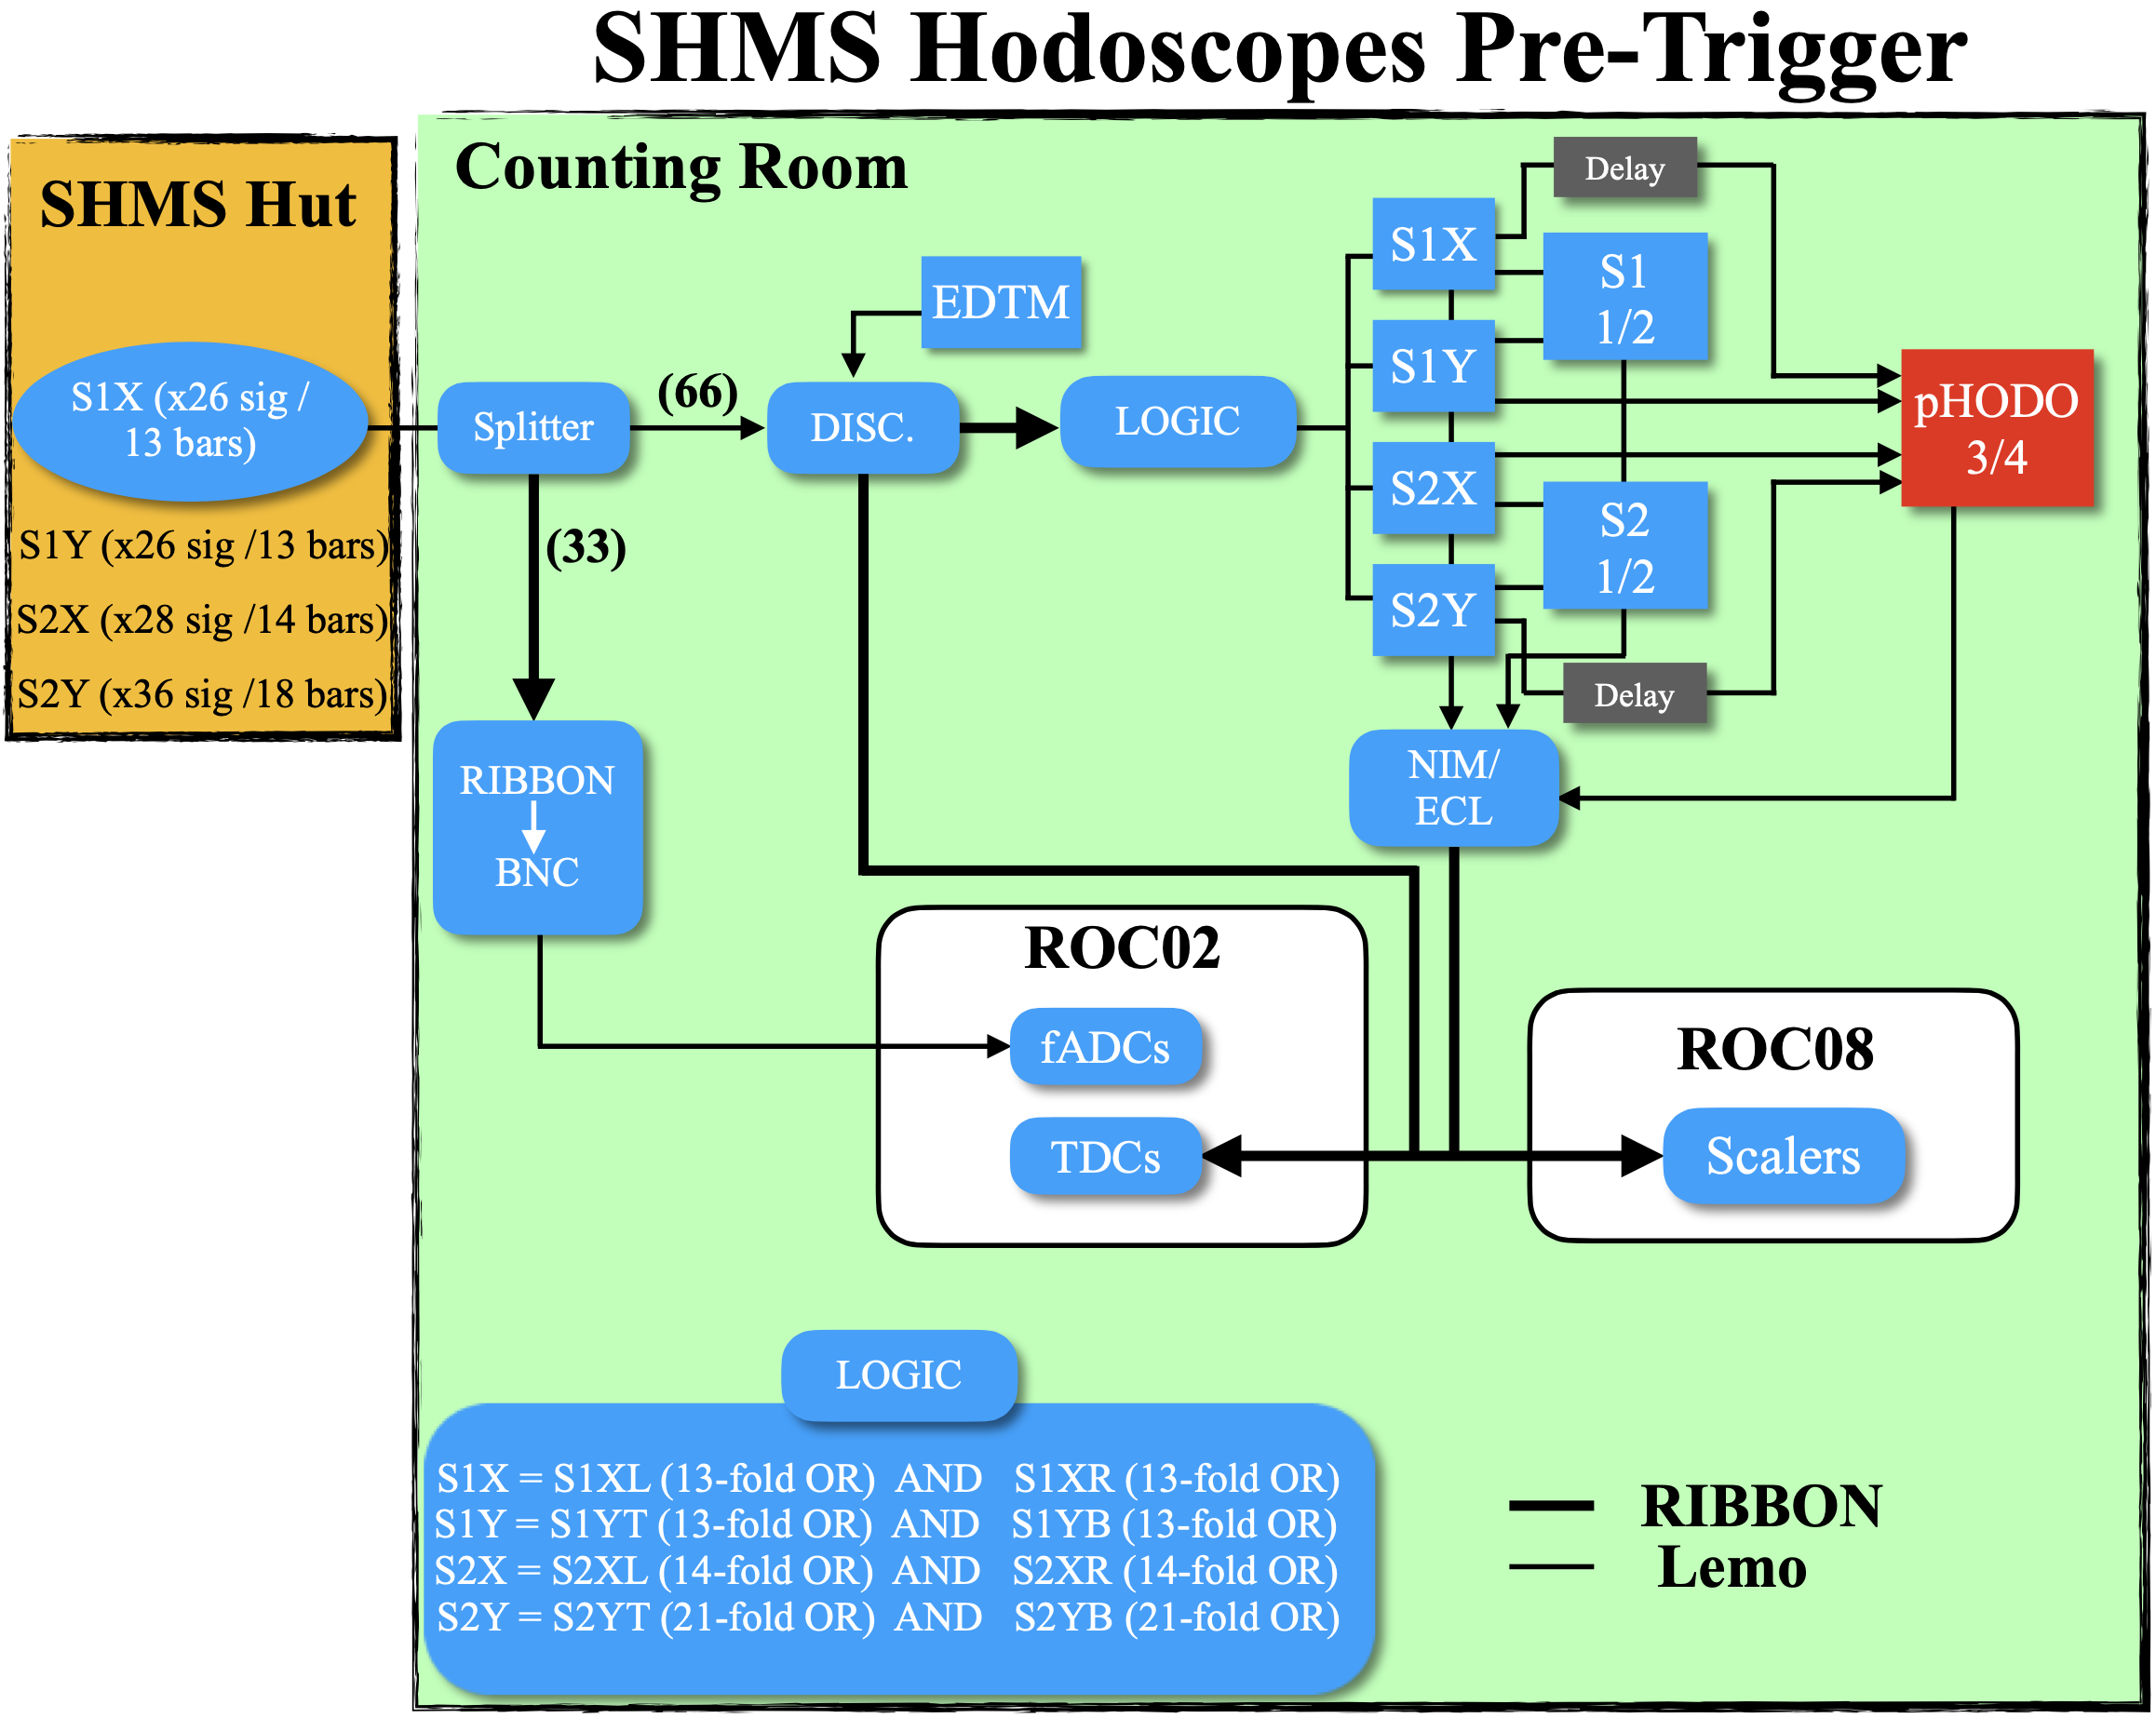
\includegraphics[scale=0.35]{pHODO_diagram.png}
  \caption{SHMS Hodoscopes Electronics Diagram. For original diagram, see Appendix \ref{appendix:Appx6}}
  \label{fig:pHODO_diagram}
\end{figure}
Each hodoscope plane consists of an array of scintillator bars coupled to a PMT at each end (See Figure \ref{fig:shms_stack}), so each bar reads out two signals. As shown in Figure \ref{fig:shms_hod_trg},
for example, hodoscope plane S1X consists of 26 signals (16 bars) read out in the Counting House (CH) patch. Each side of the plane (x13 signals/side) is fed into a 64-channel input passive splitter (16 Ch./set).
One-third (33\%) of the signal amplitude is sent via a 16-channel ribbon cable to a 64 Ch. input Ribbon-to-BNC converter (16 Ch./set) which outputs are fed into a 16-channel NIM input flash ADC (fADC).
The remaining two-thirds (66\%) of the signal amplitude is sent to a 16-Ch. input CAMAC Discriminator unit. The SHMS discriminators thresholds and gate widths were set to \shodthrs and \shodgate, respectively,
whereas the Quartz Discriminators thresholds and gate widths were set to \quartzthrs and \shodgate, respectively\\
\indent The discriminated signals are sent via two ribbon-cable outputs to CAEN1190 TDCs/Scalers (daisy-chained) and to a LeCroy 4564 CAMAC Logic unit to form the plane pre-triggers.
The Logic Unit takes four sets of 16-Ch. input ribbon cable and forms a 16-fold OR for each set by default. Further boolean operations are done through the module backplane by connecting a twisted pair cable to
the pin corresponding to the desired boolean operation. For hodoscope plane pre-triggers, the boolean operations are as follows:
\begin{empheq}[box=\fbox]{align*}
& \text{S1X = S1XL (13-fold OR) \textit{AND} S1XR (13-fold OR)} \\ 
& \text{S1Y = S1YT (14-fold OR) \textit{AND} S1YB (14-fold OR)} \\
& \text{S2X = S2XL (13-fold OR) \textit{AND} S2XR (13-fold OR)} \\ 
  & \text{S2Y = \big\{S2Y[1-16]T OR S2Y[17-21]T\big\} \textit{AND} \big\{S2Y[1-16]B OR S2Y[17-21]B\big\}}\footnotemark
\end{empheq}
\footnotetext{The SHMS S2Y (quartz) plane has 5 non-functional PMT channels on each side of the plane. In other words, it had up to 16 functional channels/side.}
\indent Once a pre-trigger has been made for each plane, they are sent to a NIM/ECL converter (Level Translator - Phillips Scientific (or P/S) Model 7126) via twisted pair cables to convert the ECL signal
(twisted pair) to a NIM signal. The NIM output is then sent to individual sets of a P/S Model 752 NIM Logic unit to adjust the widths of each of the plane pre-triggers as necessary before making a coincidence.
An X-Y hodoscope plane coincidence (S1 = S1X \textit{AND} S1Y, S2 = S2X \textit{AND} S2Y) is then made by feeding each hodoscope X-Y plane pair into a P/S Model 755 Nim Logic unit. A copy of each of the four
individual plane pre-triggers is also sent to another set of P/S Model 755 to make a 3/4 or 4/4 plane coincidence (via a front-panel knob) which defines the production hodoscope pre-trigger. A copy of all the
pre-triggers discussed above are sent to TDCs/Scalers via a NIM/ECL converter for timing and counting rate information. (See Figure \ref{fig:pHODO_diagram}) \\

\subsection{Pre-Shower / Shower Calorimeter Pre-Trigger}
\begin{figure}[h!]
  \centering
  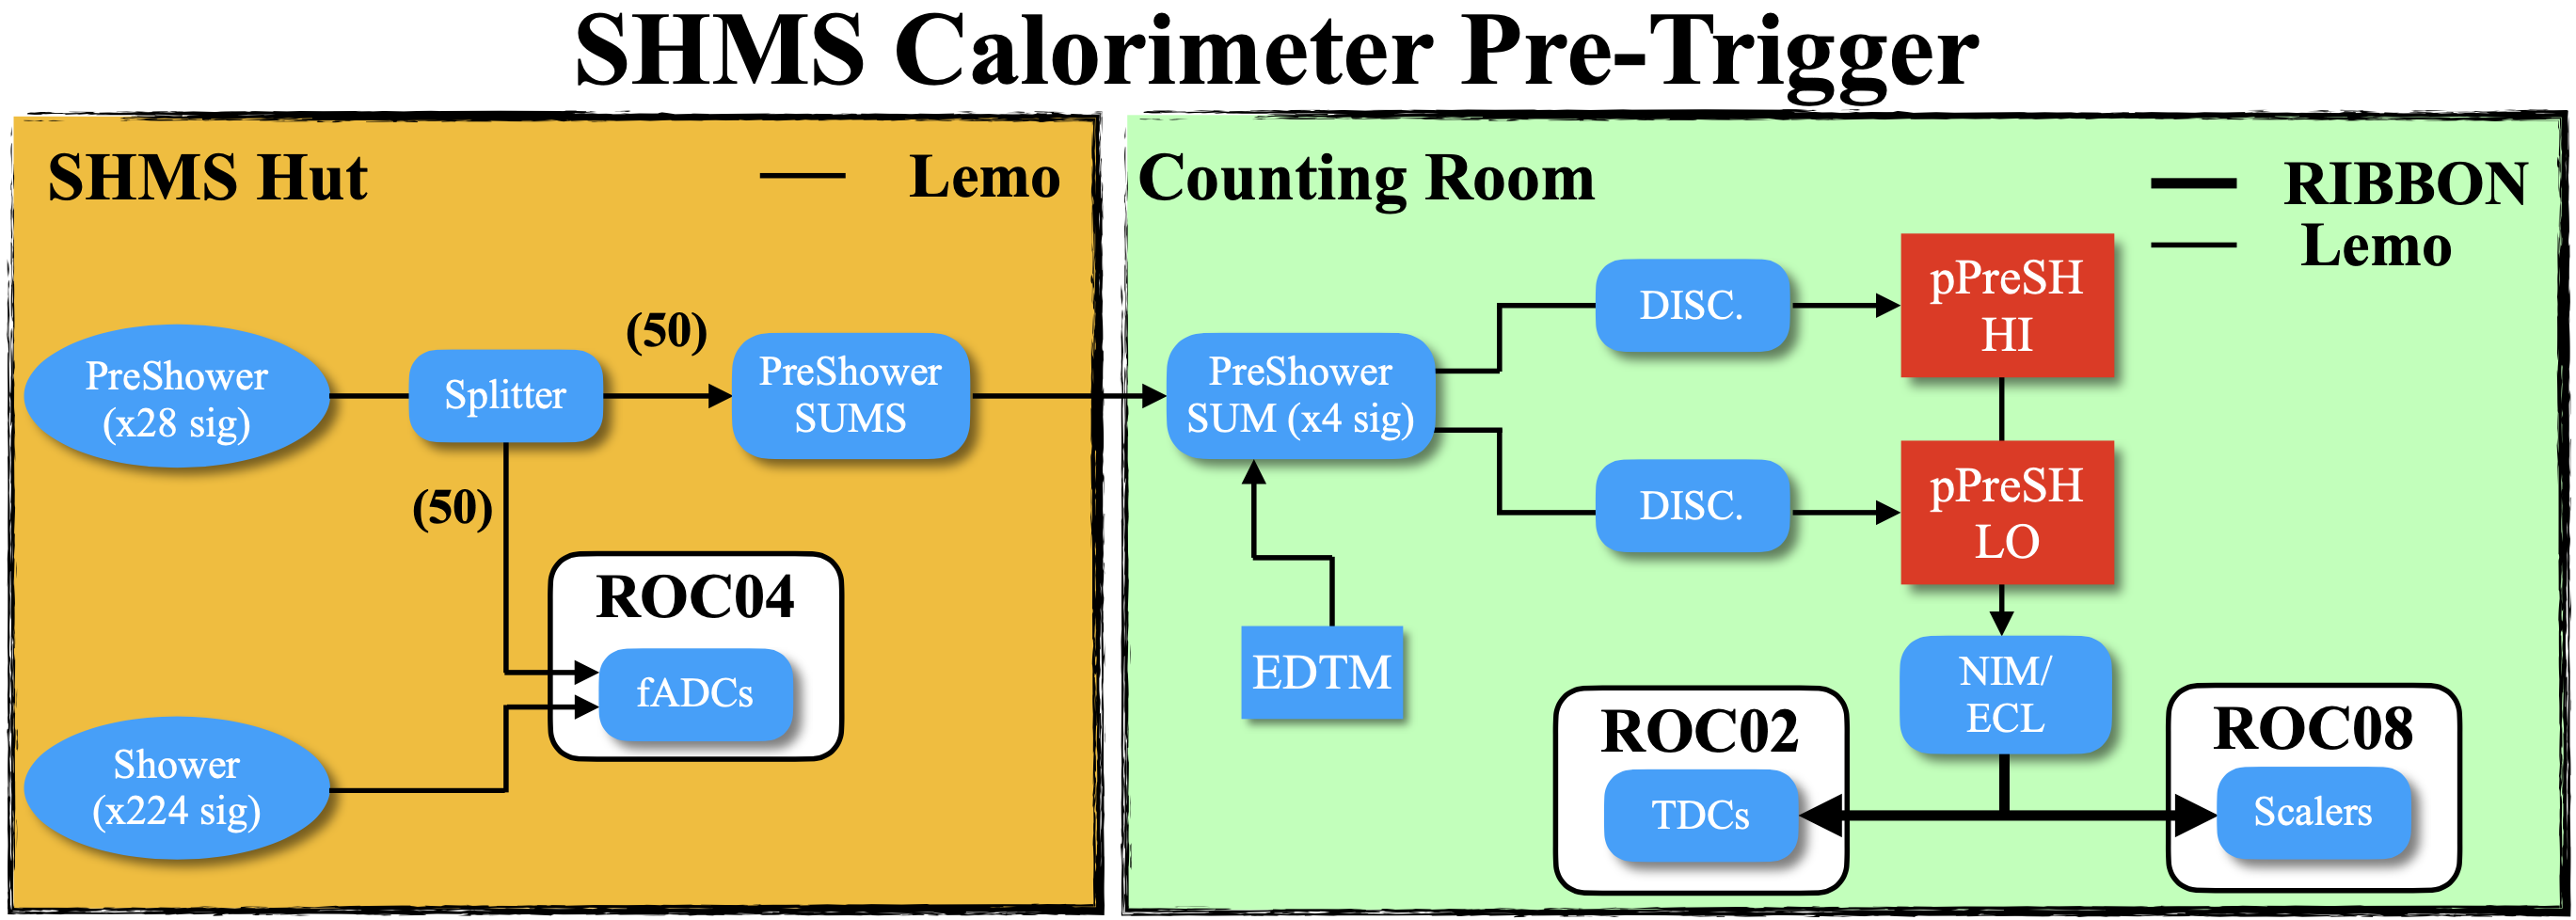
\includegraphics[scale=0.35]{pCAL_diagram.png}
  \caption{SHMS PreShower / Shower Electronics Diagram. For original diagram, see Appendix \ref{appendix:Appx7}}
  \label{fig:pCAL_diagram}
\end{figure}

The SHMS Pre-Shower consists of two sets of fourteen (PMT-coupled) lead blocks oriented perpendicular to the Shower Counter blocks\cite{shms_preSh_talk}. The initial sum was done in the SHMS Electronics Hut. PMT signals
from groups of four blocks were summed to form:
\begin{empheq}[box=\fbox]{align*}
  & \text{preSh SUM [1-4]: [1-4]L + [1-4]R} \\ 
  & \text{preSh SUM [5-8]: [5-8]L + [5-8]R} \\ 
  & \text{preSh SUM [9-12]: [9-12]L + [9-12]R} \\ 
  & \text{preSh SUM [13-14]: [13-14]L + [13-14]R}
\end{empheq}
The Shower counter consists of 224 lead blocks, each coupled to a PMT at the end. Becasue of the high channel density of this detector, its signals are sent
directly to the ROC 4 fADCs in the SHMS detector hut.
\newpage
\subsection{Heavy/Noble Gas \v{C}erenkov Pre-Trigger}
\begin{figure}[h!]
  \centering
  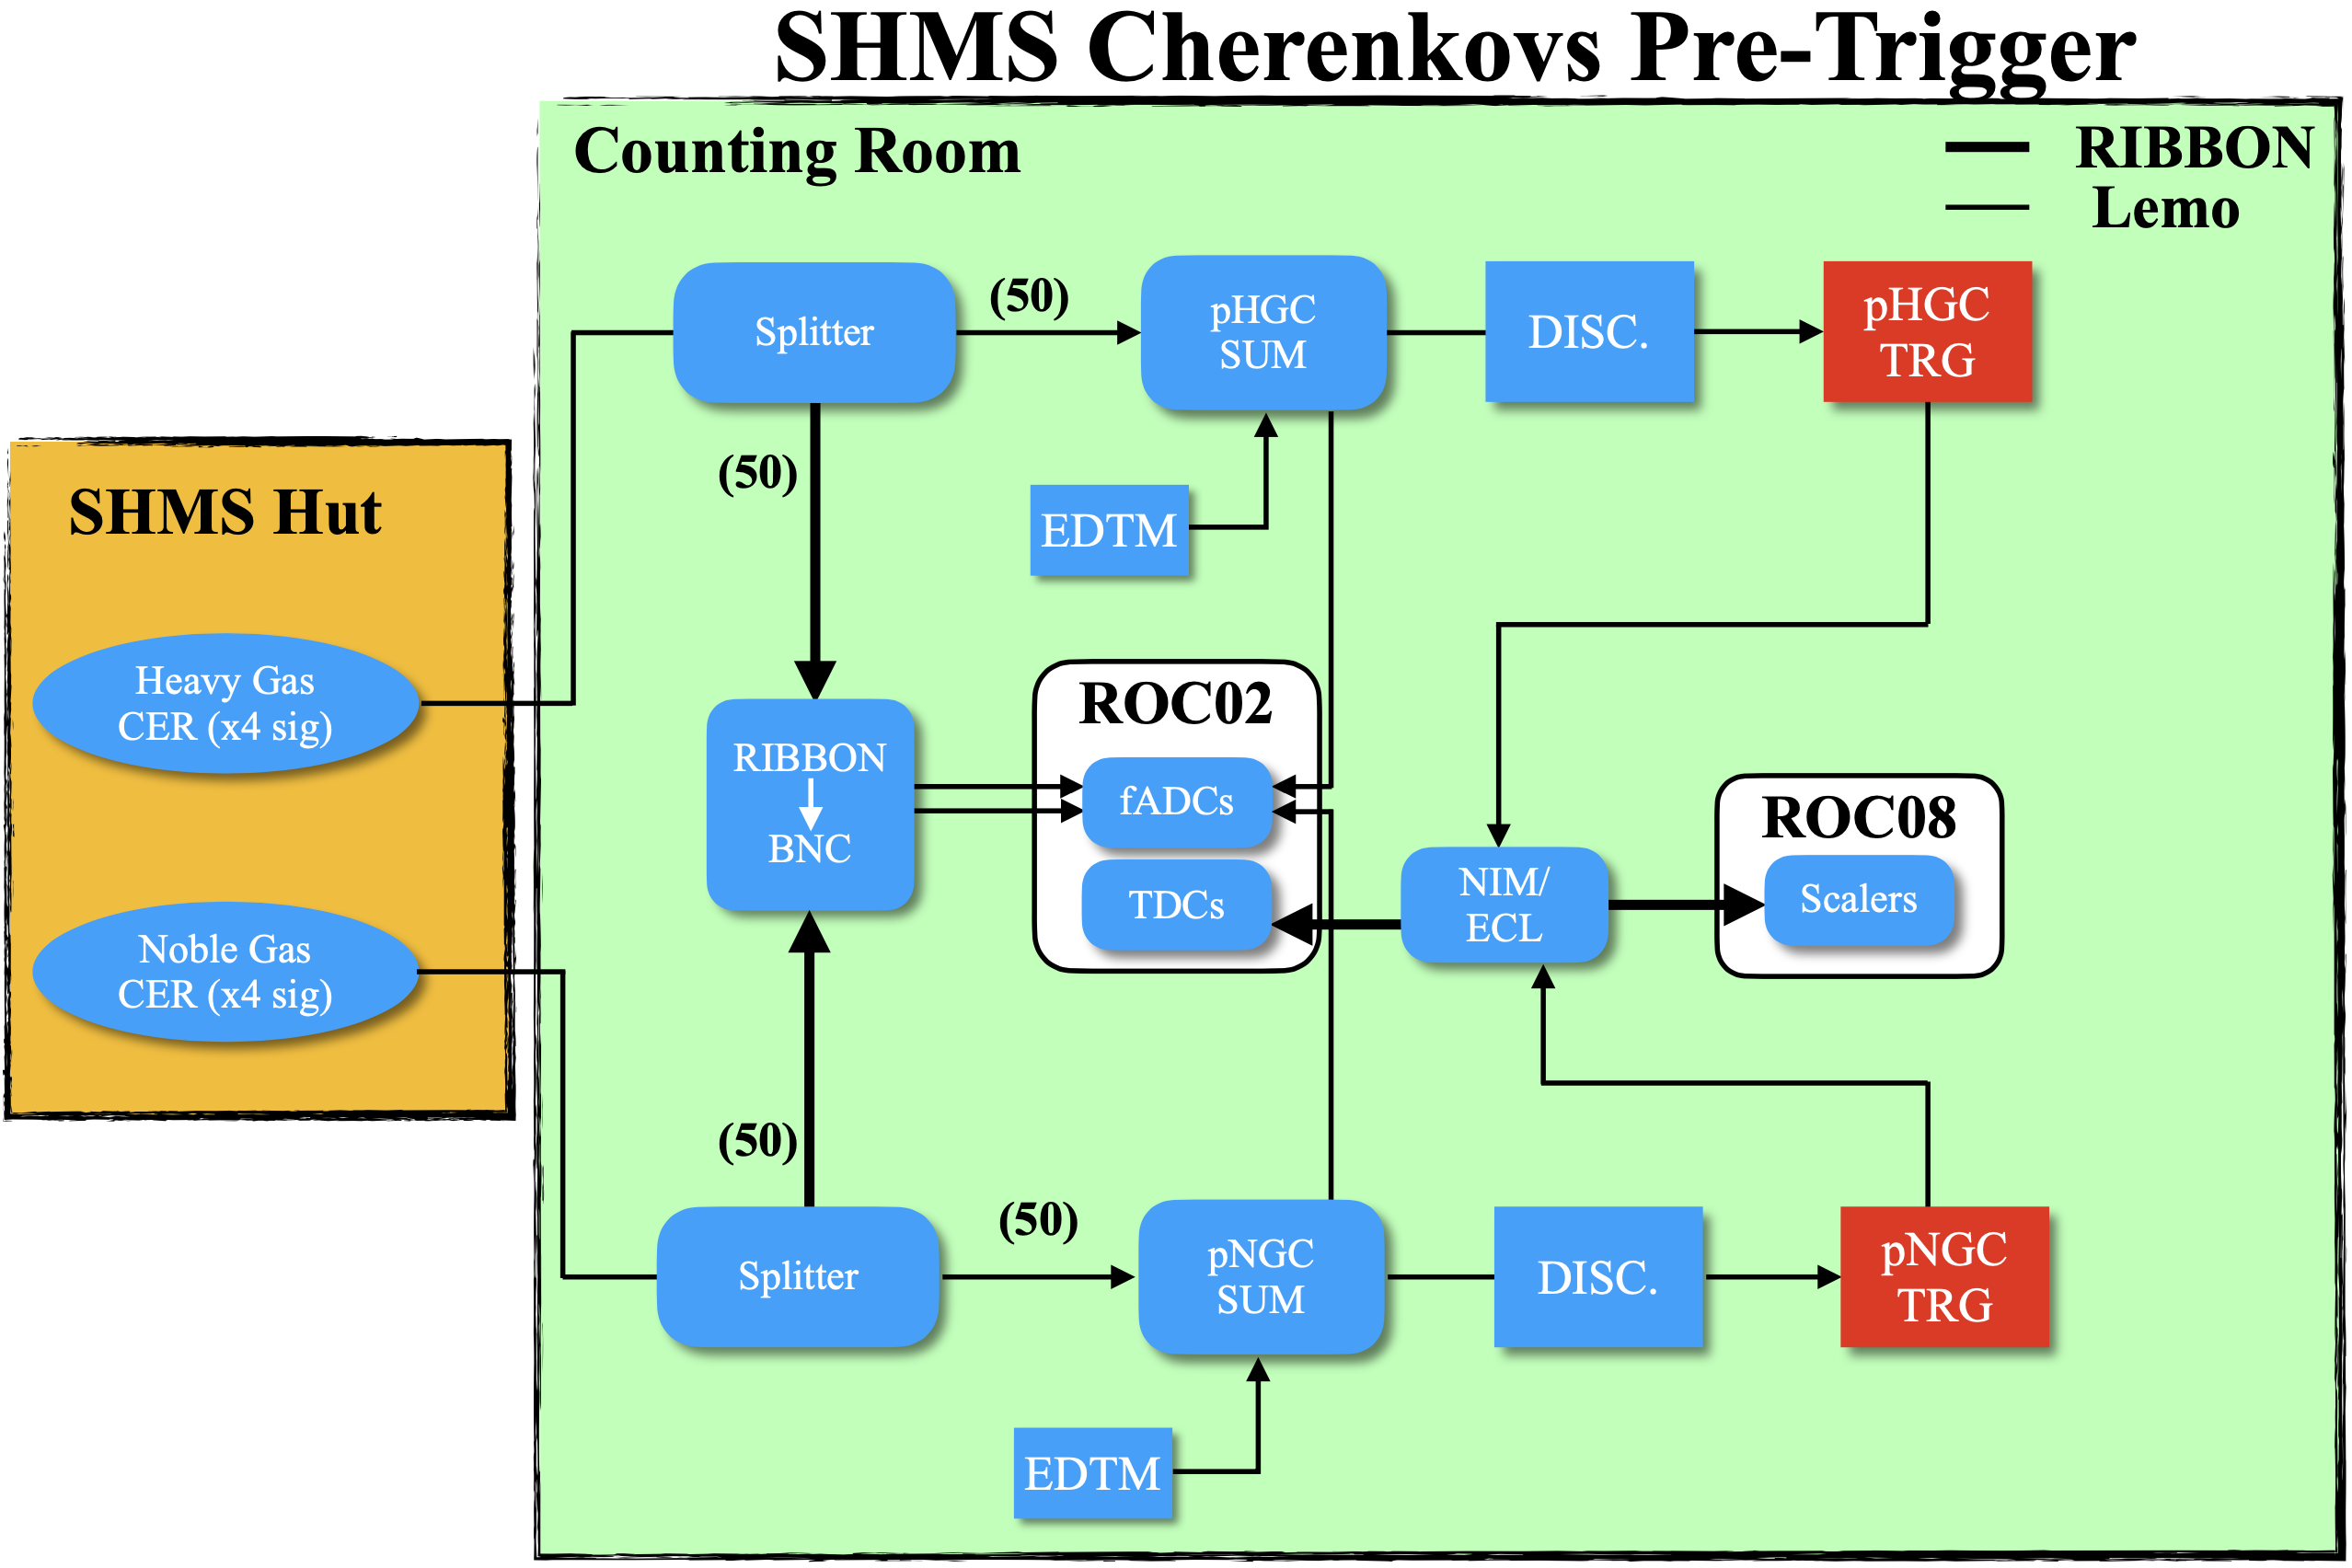
\includegraphics[scale=0.35]{pCER_diagram.png}
  \caption{SHMS Gas \v{C}erenkovs Electronics Diagram.}
  \label{fig:pCER_diagram}
\end{figure}
\noindent The SHMS Heavy Gas \v{C}erenkov detector consists of a 1 m long, 1.6 m in diameter cylindrical tank located between the first set of hodoscope planes and the Aerogel (See Figure \ref{fig:shms_stack}).
The tank is filled with a gas and has four thin spherical mirrors that focus the \v{C}erenkov photons towards four 5-inch PMTs\cite{shms_hgc_talk}. 
\newline
\indent The SHMS Noble Gas \v{C}erenkov detector consists of a 2 m long active length of Argon/Neon gas tank located before the first drift chamber (See Figure \ref{fig:shms_stack}).
The tank is filled with a gas and has four overlapping mirrors, that focus the \v{C}erenkov photons towards four 5-inch PMTs\cite{shms_ngc_talk}. 
For the original electronics diagram, See Appendix \ref{appendix:Appx4} on the HMS Gas \v{C}erenkov.
\subsection{Aerogel \v{C}erenkov Pre-Trigger}
\indent The SHMS Aerogel \v{C}erenkov detector consists of a 110 x 100 x 24.5 cm$^{3}$ rectangular aerogel tray coupled to a diffusion box. The diffusion box has seven 5-inch PMTs on each side
which detect \v{C}erenkov light produced by interactions with the Aerogel material\cite{shms_aero_article}. The detector is located between Heavy Gas \v{C}erenkov and second set of hodoscope planes
(See Figure \ref{fig:shms_stack}). The electronics diagram is the same as in Figure \ref{fig:pCER_diagram}. For the original diagram, see Appendix \ref{appendix:Appx4}
\newpage
\subsection{SHMS Single Arm Pre-Trigger}
\begin{figure}[h!]
  \centering
  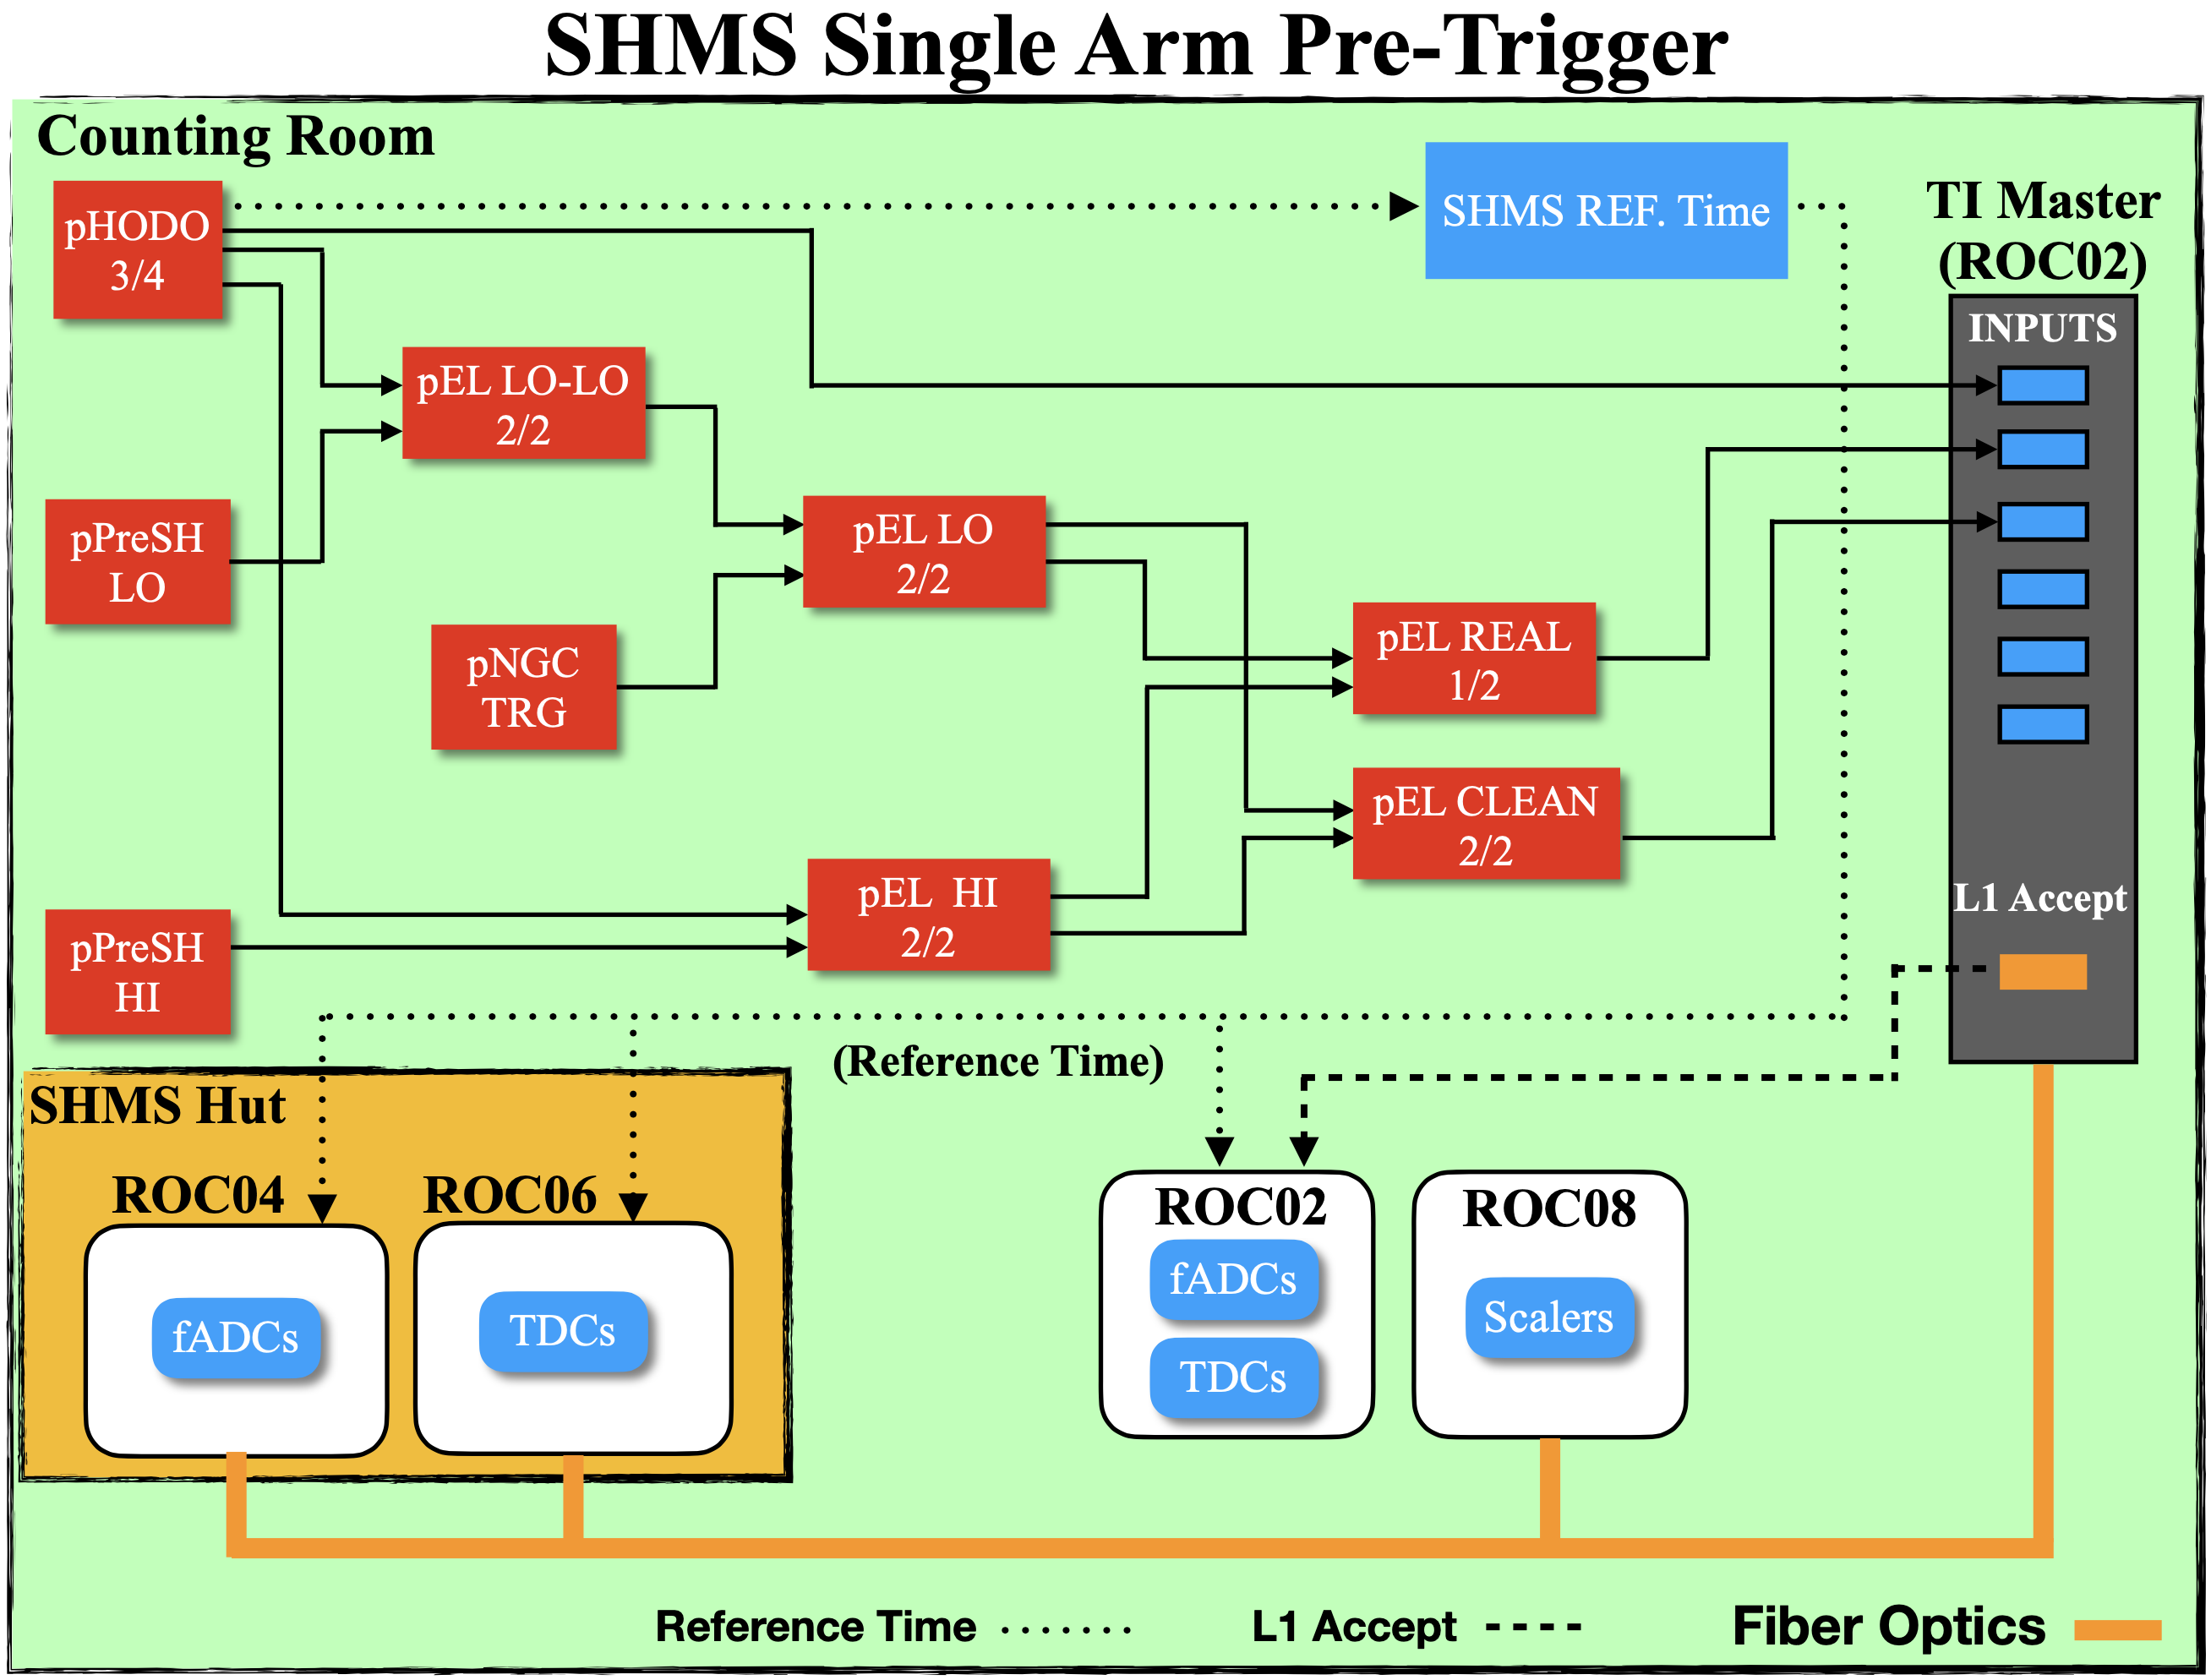
\includegraphics[scale=0.35]{SHMS_SingleArm_diagram.png}
  \caption{SHMS Single Arm Trigger Electronics Diagram. For the original diagram, see Appendix \ref{appendix:Appx8}.}
  \label{fig:SHMS_SingleArm_diagram}
\end{figure}

\indent The SHMS single arm trigger is be formed exactly as the HMS single arm trigger, with the exception of the detectors involved. Compare the electronics diagrams in Figures \ref{fig:SHMS_SingleArm_diagram} and
\ref{fig:HMS_SingleArm_diagram}, and read Section \ref{ssec:hms_single_arm_sec} for a detailed description of the electronic diagrams. 
\newpage
\section{Coincidence Trigger Set-Up}
\begin{figure}[h!]
  \centering
  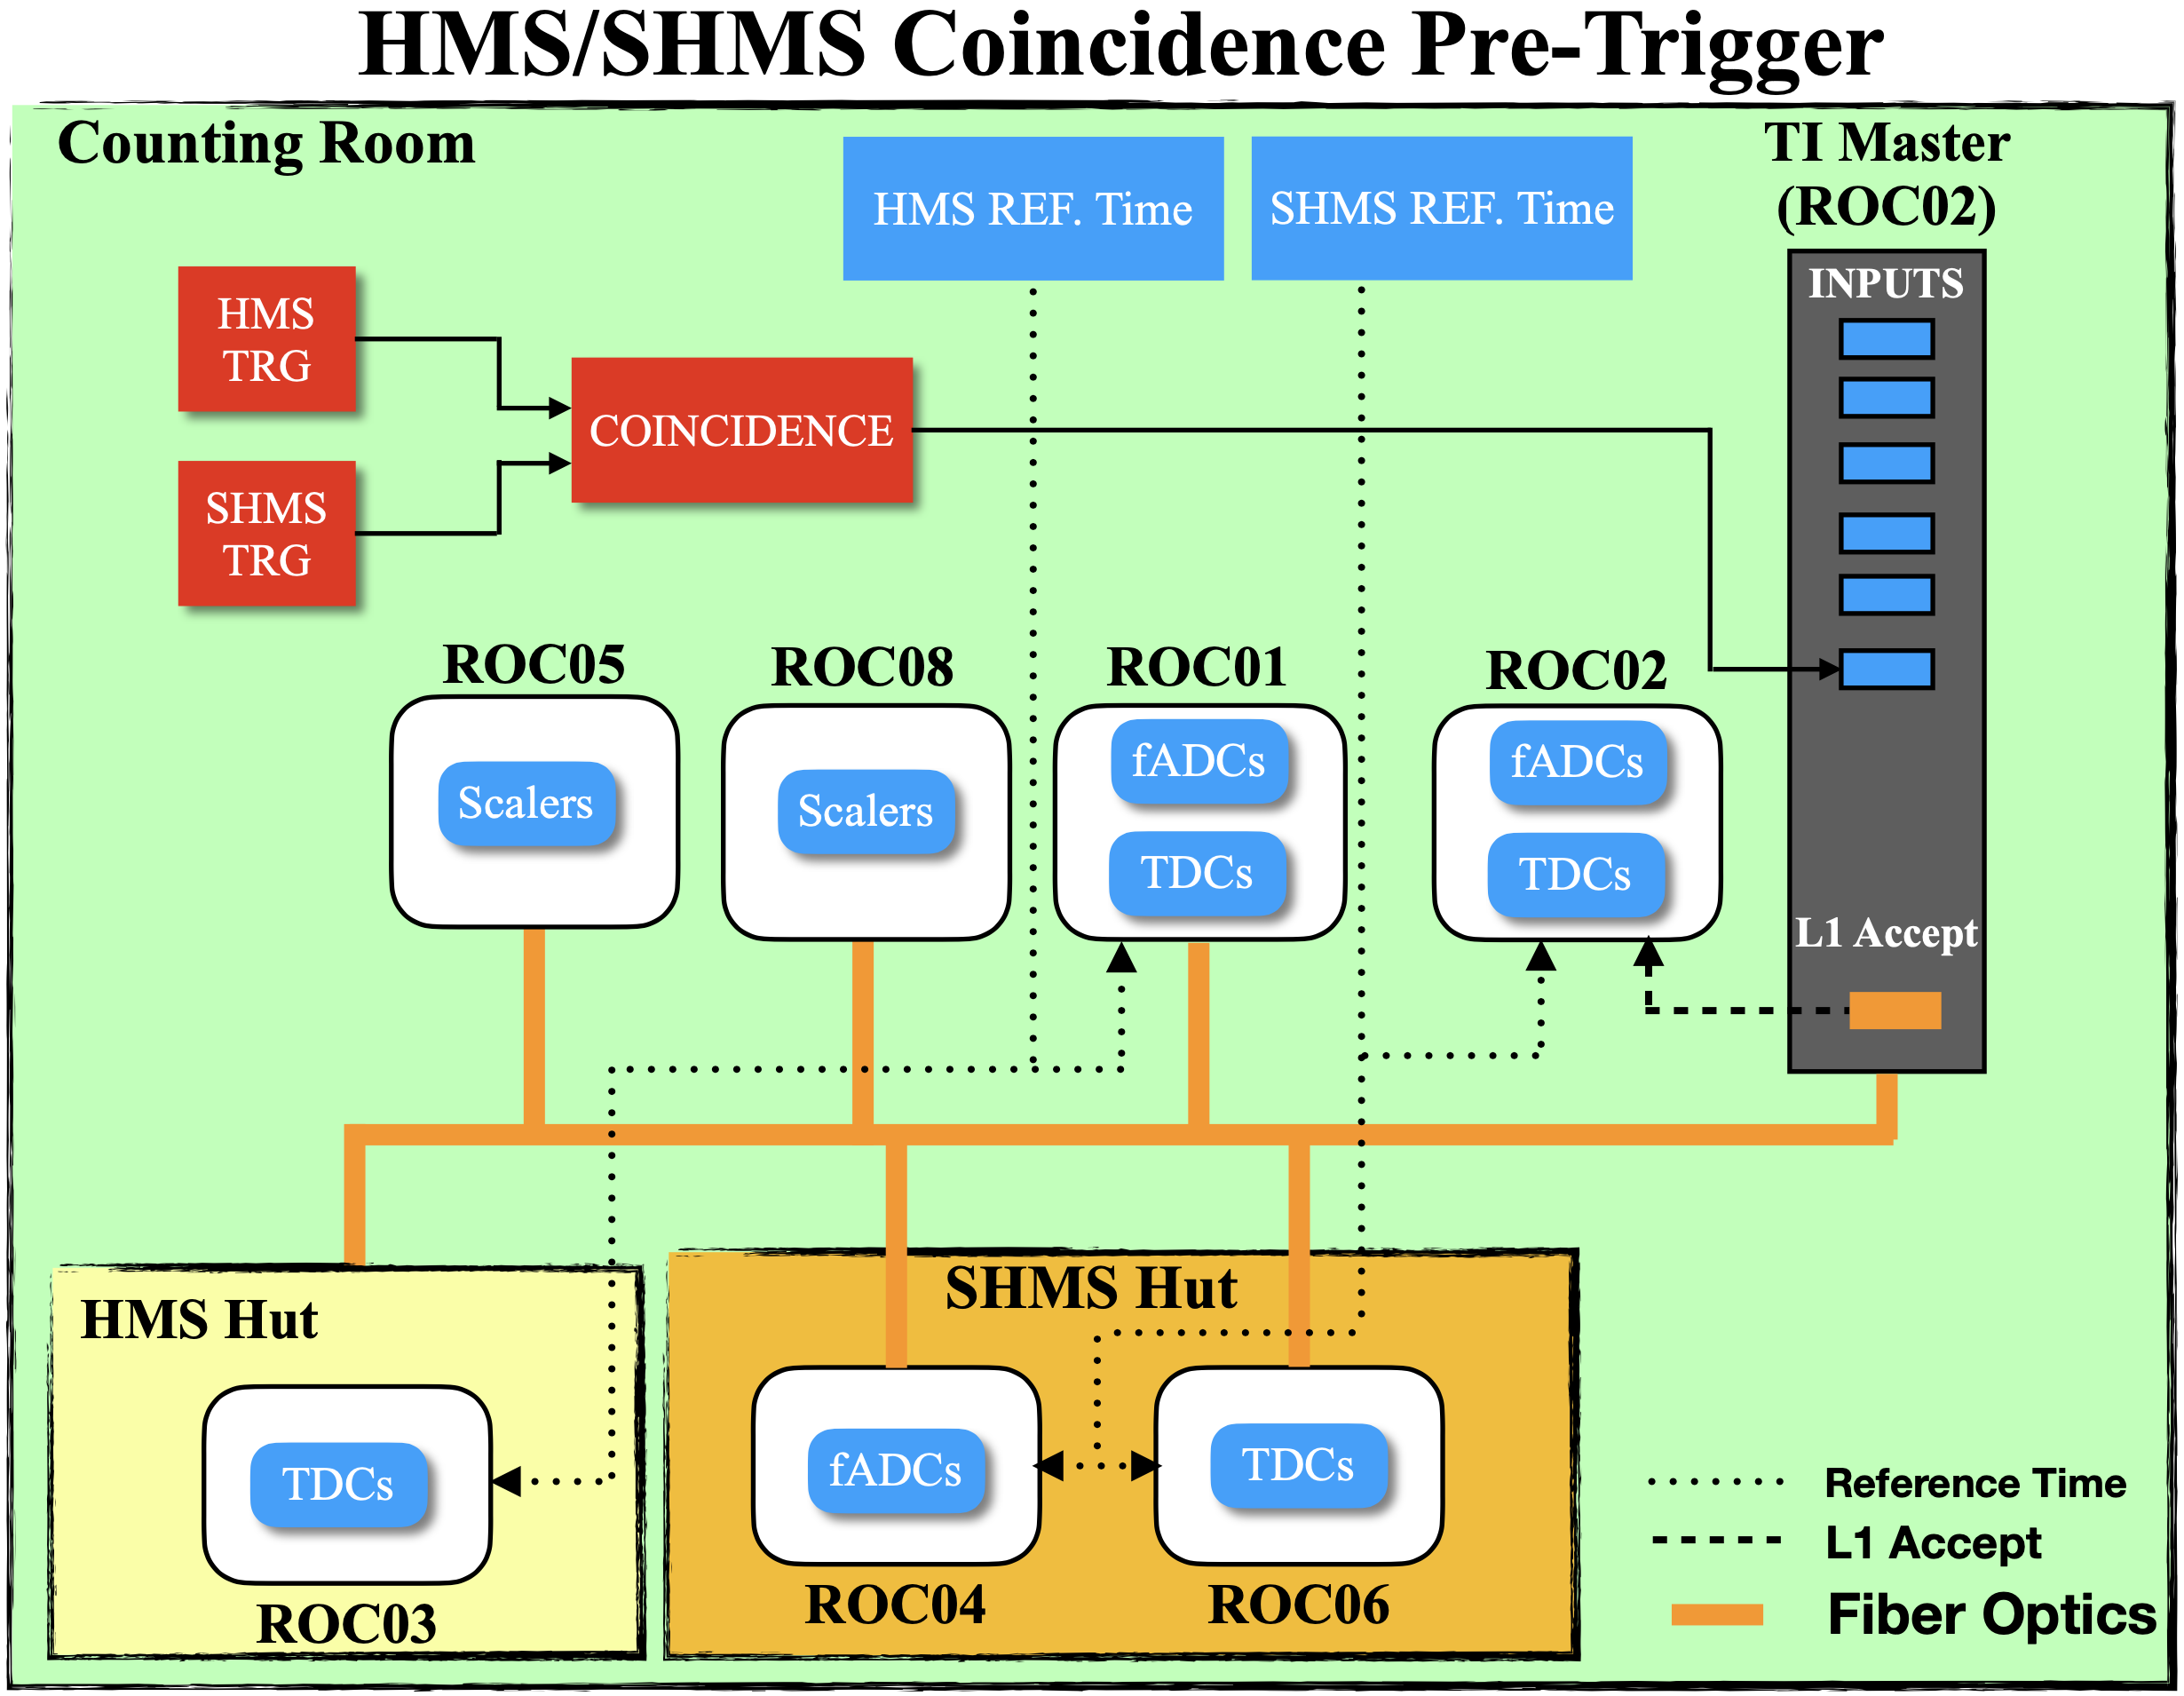
\includegraphics[scale=0.35]{Coin_diagram.png}
  \caption{Coincidence Trigger Electronics Diagram. For the original diagram, see Appendix \ref{appendix:Appx9}}
  \label{fig:Coin_TRG}
\end{figure}
\indent In coincidence mode, the HMS and SHMS pre-triggers are sent to a NIM Logic module, where the first pre-trigger that arrives will open
a coincidence time window during which the second pre-trigger may or may not arrive in time. This will determine whether two events that occurred in
each spectrometer are correlated with the event that originated at the target. If the coincidence pre-trigger is formed, a copy will be sent to
scalers and TDCs, while the other copy is sent to a NIM/ECL converter where three copies (may be more) are sent via twisted pairs to every TDC module and the TI, which will be the \textbf{ONLY} Trigger Master in coincidence mode. Additional copies (not shown) may need to be sent to the HMS readout crate (ROC 01) as well, since the coincidence pre-trigger\footnote{A copy of the coincidence pre-trigger will also need to be sent to the
  HMS/SHMS TDC modules present in the detector huts crates via the patch panel.} is common to all crates. \\
\indent Once the coincidence pre-trigger is processed by the TI Master in ROC 02, it is sent to a NIM/ECL converter, where a copy is sent to scalers and TDCs, and the other copy is sent to the ``TRG'' NIM input in the TDC front panel, and daisy-chained with other TDCs in ROC02 and ROC01. The remaining crates in the HMS/SHMS huts receive a copy of the accepted trigger via fiber optics lines running from the TI Master to the TIs in all other crates. The TIs then distribute the accepted trigger to all modules of their respective crates.

\section{Electronic Dead Time Monitoring (EDTM)}\label{sec:edtm}
\noindent The EDTM system is a new method used in Hall C to measure the total dead time of the data acquisition (DAQ) system. It consists of introducing a controlled (fixed frequency) pulse
as near as possible to the detectors that form part of the trigger. Ideally, one would send the EDTM pulses at the detector level in the hut such that both the real physics and EDTM signals
pass through the same electronics. Since this is not easy or practical to do, the EDMT logic pulses are injected at the trigger logic level in the Counting Room.\\
\begin{figure}[H]
  \centering
  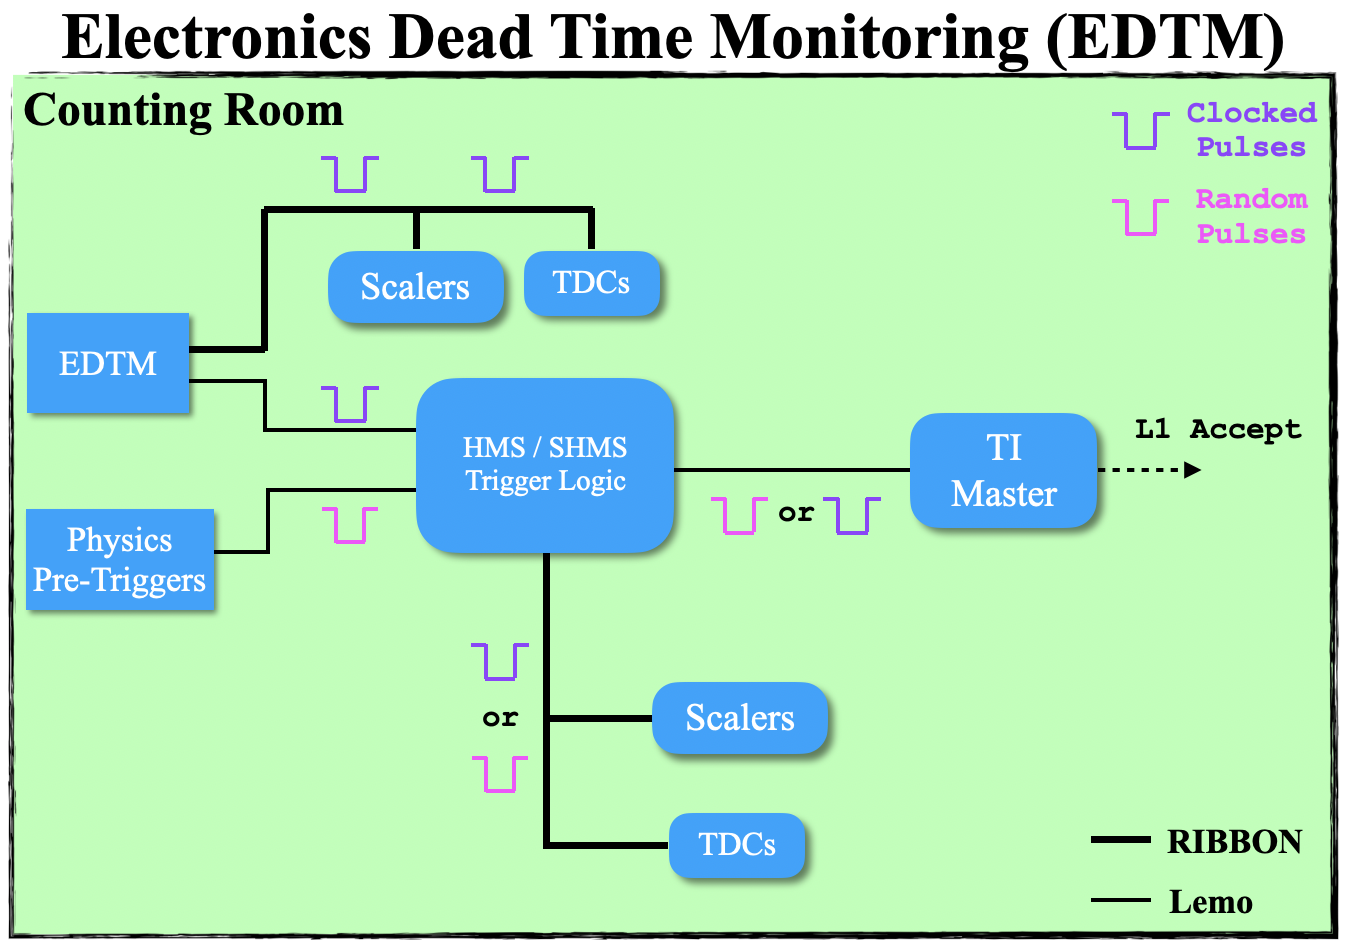
\includegraphics[scale=0.54]{EDTM_diagram.png}
  \caption{EDTM electronics diagram.}
  \label{fig:EDTM_diagram}
\end{figure}
\indent By design, the EDTM is a \textit{real} trigger as measured by the electronics and readout systems. Since the EDTM is invasive to the trigger electronics, its frequency should be small
enough to minimize the probability of blocking actual physics triggers, but sufficiently large to gather the necessary statistics for a precise \textit{dead time} measurement during the course of a run. \\
\indent Figure \ref{fig:EDTM_diagram} shows a simplified diagram of the EDTM signal distribution through the trigger electronics. The EDTM logic signals (purple) are injected into the trigger logic
where they mix with the physics pre-triggers (magenta). A separate copy of the EDTM is also sent to scalers/TDCs to be used in the dead time calculation. If the
EDTM makes it to the front-end of the Trigger Interface (TI) module and gets accepted (L1 Accept), it has esentially measured both the electronics and computer dead time.\\
\begin{figure}[H]
  \centering
  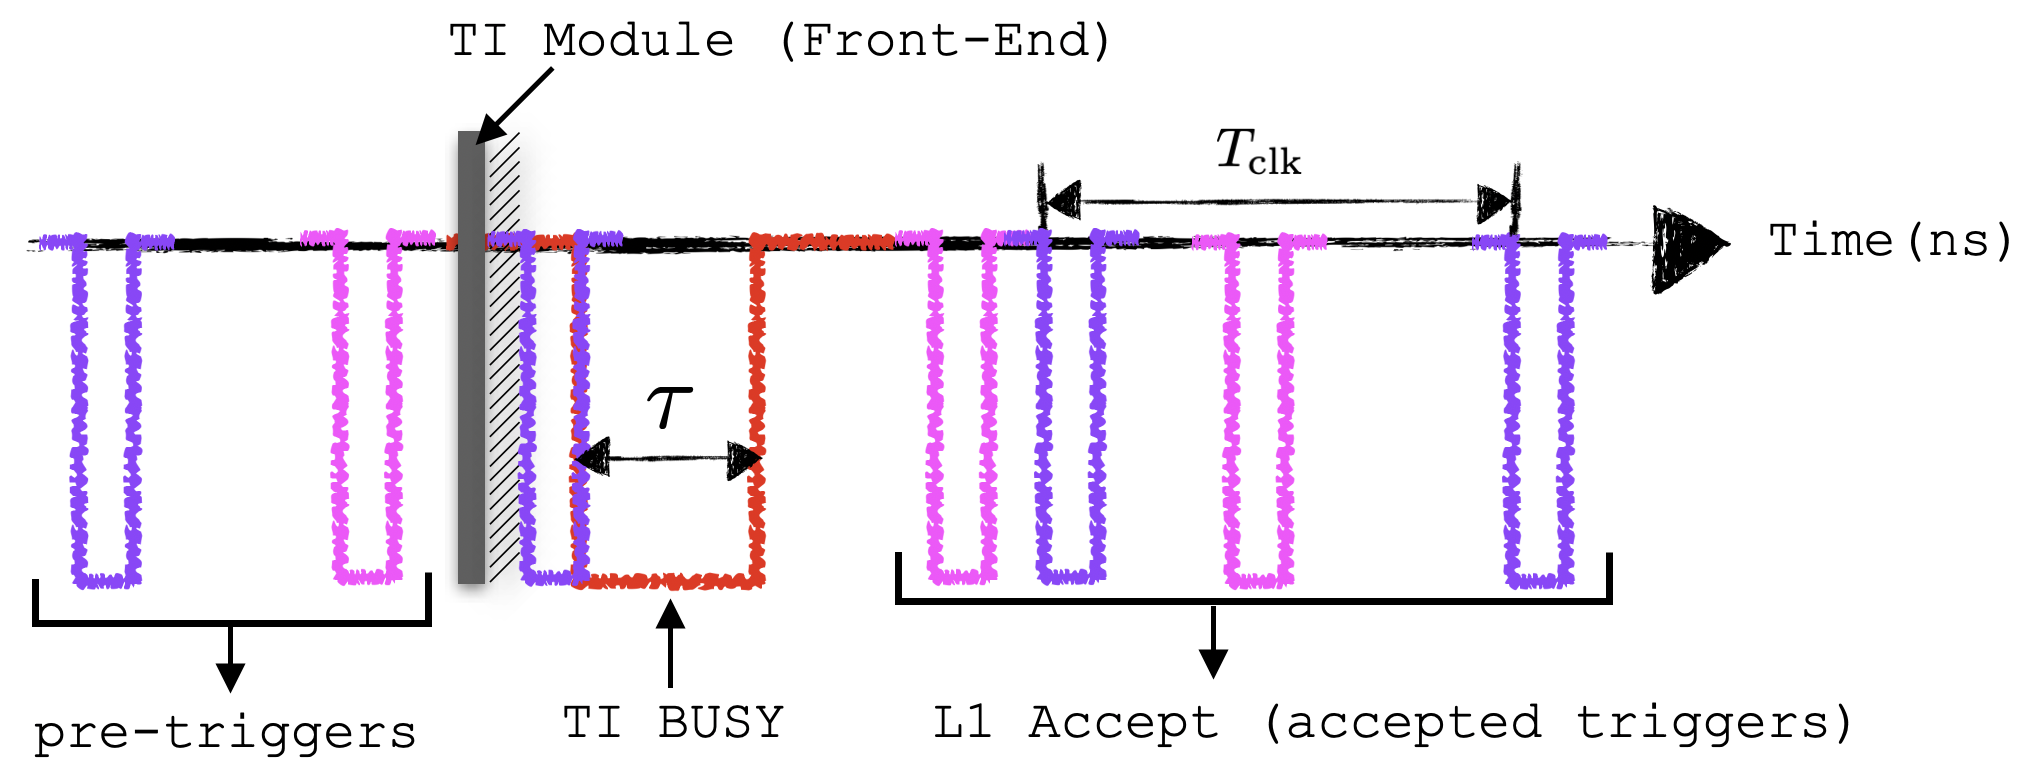
\includegraphics[scale=0.40]{EDTM_TI.png}
  \caption{Cartoon representation of EDTM (purple) and physics (magenta) pre-triggers at the TI module front-end.}
  \label{fig:EDTM_TI}
\end{figure}\\
\indent Figure \ref{fig:EDTM_TI} shows the random physics (magenta) and clocked (purple) EDTM pulses at an input channel of the TI front-end where the EDTM has
been set to a sufficiently large frequency ($1/T_{\mathrm{clk}}$) to ensure that enough EDTM signals get accepted in order to make a statistically significant and
reliable dead time calculation. In this example, an EDTM signal has been accepted by the TI which triggered a \textit{BUSY} signal for a time $\tau$ during which all other incoming pre-triggers are blocked
contributing to the DAQ computer dead time. The accepted pre-triggers are distributed to all ROCs for data readout. \\
\indent Over the course of a run, the total dead time ($T_{\mathrm{TDT}}$), or alternatively, the total live time ($T_{\mathrm{TLT}}$) in terms of the EDTM is defined as
\begin{equation}
 T_{\mathrm{TDT}} \equiv 1 - T_{\mathrm{TLT}} = 1 - \frac{N_{\mathrm{edtm,acc}}}{N_{\mathrm{edtm,scl}}},
  \label{eq:3.24}
\end{equation}
where $N_{\mathrm{edtm,acc}}$ is the number of accepted EDTM counts obtained by requiring a non-zero hit on the EDTM TDC spectrum, and $N_{\mathrm{edtm,scl}}$ is the number of EDTM scaler counts regardless of whether or not
the EDTM was accepted. In reality, frequent beam trips occur during the course of a run which makes this calculation biased since one can measure live times of $\sim$100$\%$ during beam-off periods as only
the EDTM signal (and cosmic rays) are measured. To eliminate this bias, the live time calculation was done by making a software cut on the beam current above a certain threshold.
Furthermore, since the EDTM events are generated by a clock, rather than a poisson source, it introduces an additional bias since the EDTM cannot block itself. To account for this bias, an additional correction
to the total live time was derived and can be found in Ref.\cite{DMack_livetime_2019}. This correction, however, is negligible provided that the EDTM rate is sufficiently low as was the case for this experiment ($\sim 2$ Hz). \\
\indent Even though only the total live time is required as a correction factor in the measured cross section, one may also calculate the computer live time defined as
\begin{equation}
  T_{\mathrm{CLT}} = \frac{N_{\mathrm{phy,acc}}}{N_{\mathrm{phy,scl}}},
  \label{eq:3.25}
\end{equation}
where $N_{\mathrm{phy,acc}}$ is the number of accepted physics triggers obtained by requiring a zero hit on the EDTM TDC spectrum (EDTM rejected by TI) and $N_{\mathrm{phy,scl}}$ is the number of physics trigger scaler counts after
having subtracted the EDTM scaler counts. The electronic live time can then be obtained from the following formula:
\begin{equation}
  T_{\mathrm{TLT}} = T_{\mathrm{CLT}} \cdot T_{\mathrm{ELT}},
  \label{eq:3.26}
\end{equation}
where $T_{\mathrm{ELT}}$ is the electroninc live time expressed as a fraction (not percent). \\
\indent For a more detailed discussion on the live time calculations and its correction factors
see Refs.\cite{pooser_livetime_2019,DMack_livetime_2019}.
\newpage
\textcolor{red}{\section{Notes on Changes to the Trigger}}\label{sec:trg_ch}
\indent In Hall C, each spectrometer has multiple pre-triggers (HODO 3/4, STOF, EL-REAL, EL-CLEAN) that may change depending on the nature of the experiment.
The base pre-trigger is the HODO 3/4, which requires at least 3 of 4 hodoscope planes to fire. Since the commissioning phase (Fall 2017) of the spectrometers, the trigger
electronics has had three major modifications up to the present time (Fall 2020) described below.\\
\indent During the commissioning phase of the spectrometers, the reference time logic was initially defined to be:
\begin{align}
  T^{\mathrm{logic}}_{\mathrm{reftime,init}} \equiv &\textbf{ p(h)HODO 3/4} \text{ OR } \textbf{p(h)STOF} \nonumber  \\
  &\text{ OR } \textbf{p(h)EL-REAL} \text{ OR } \textbf{p(h)EL-CLEAN}
  \label{eq:refTime_def1}
\end{align}
where the logic pre-trigger signals described in Eq. \ref{eq:refTime_def1} have been delayed in time relative to each other and the \textbf{p(h)} refers to prefix used in the software to denote the SHMS (HMS).\\
\subsection{January, 2018: Removal of STOF from Reference Time Definition}\label{ssec:jan2018}
\begin{figure}[H]
  \centering
  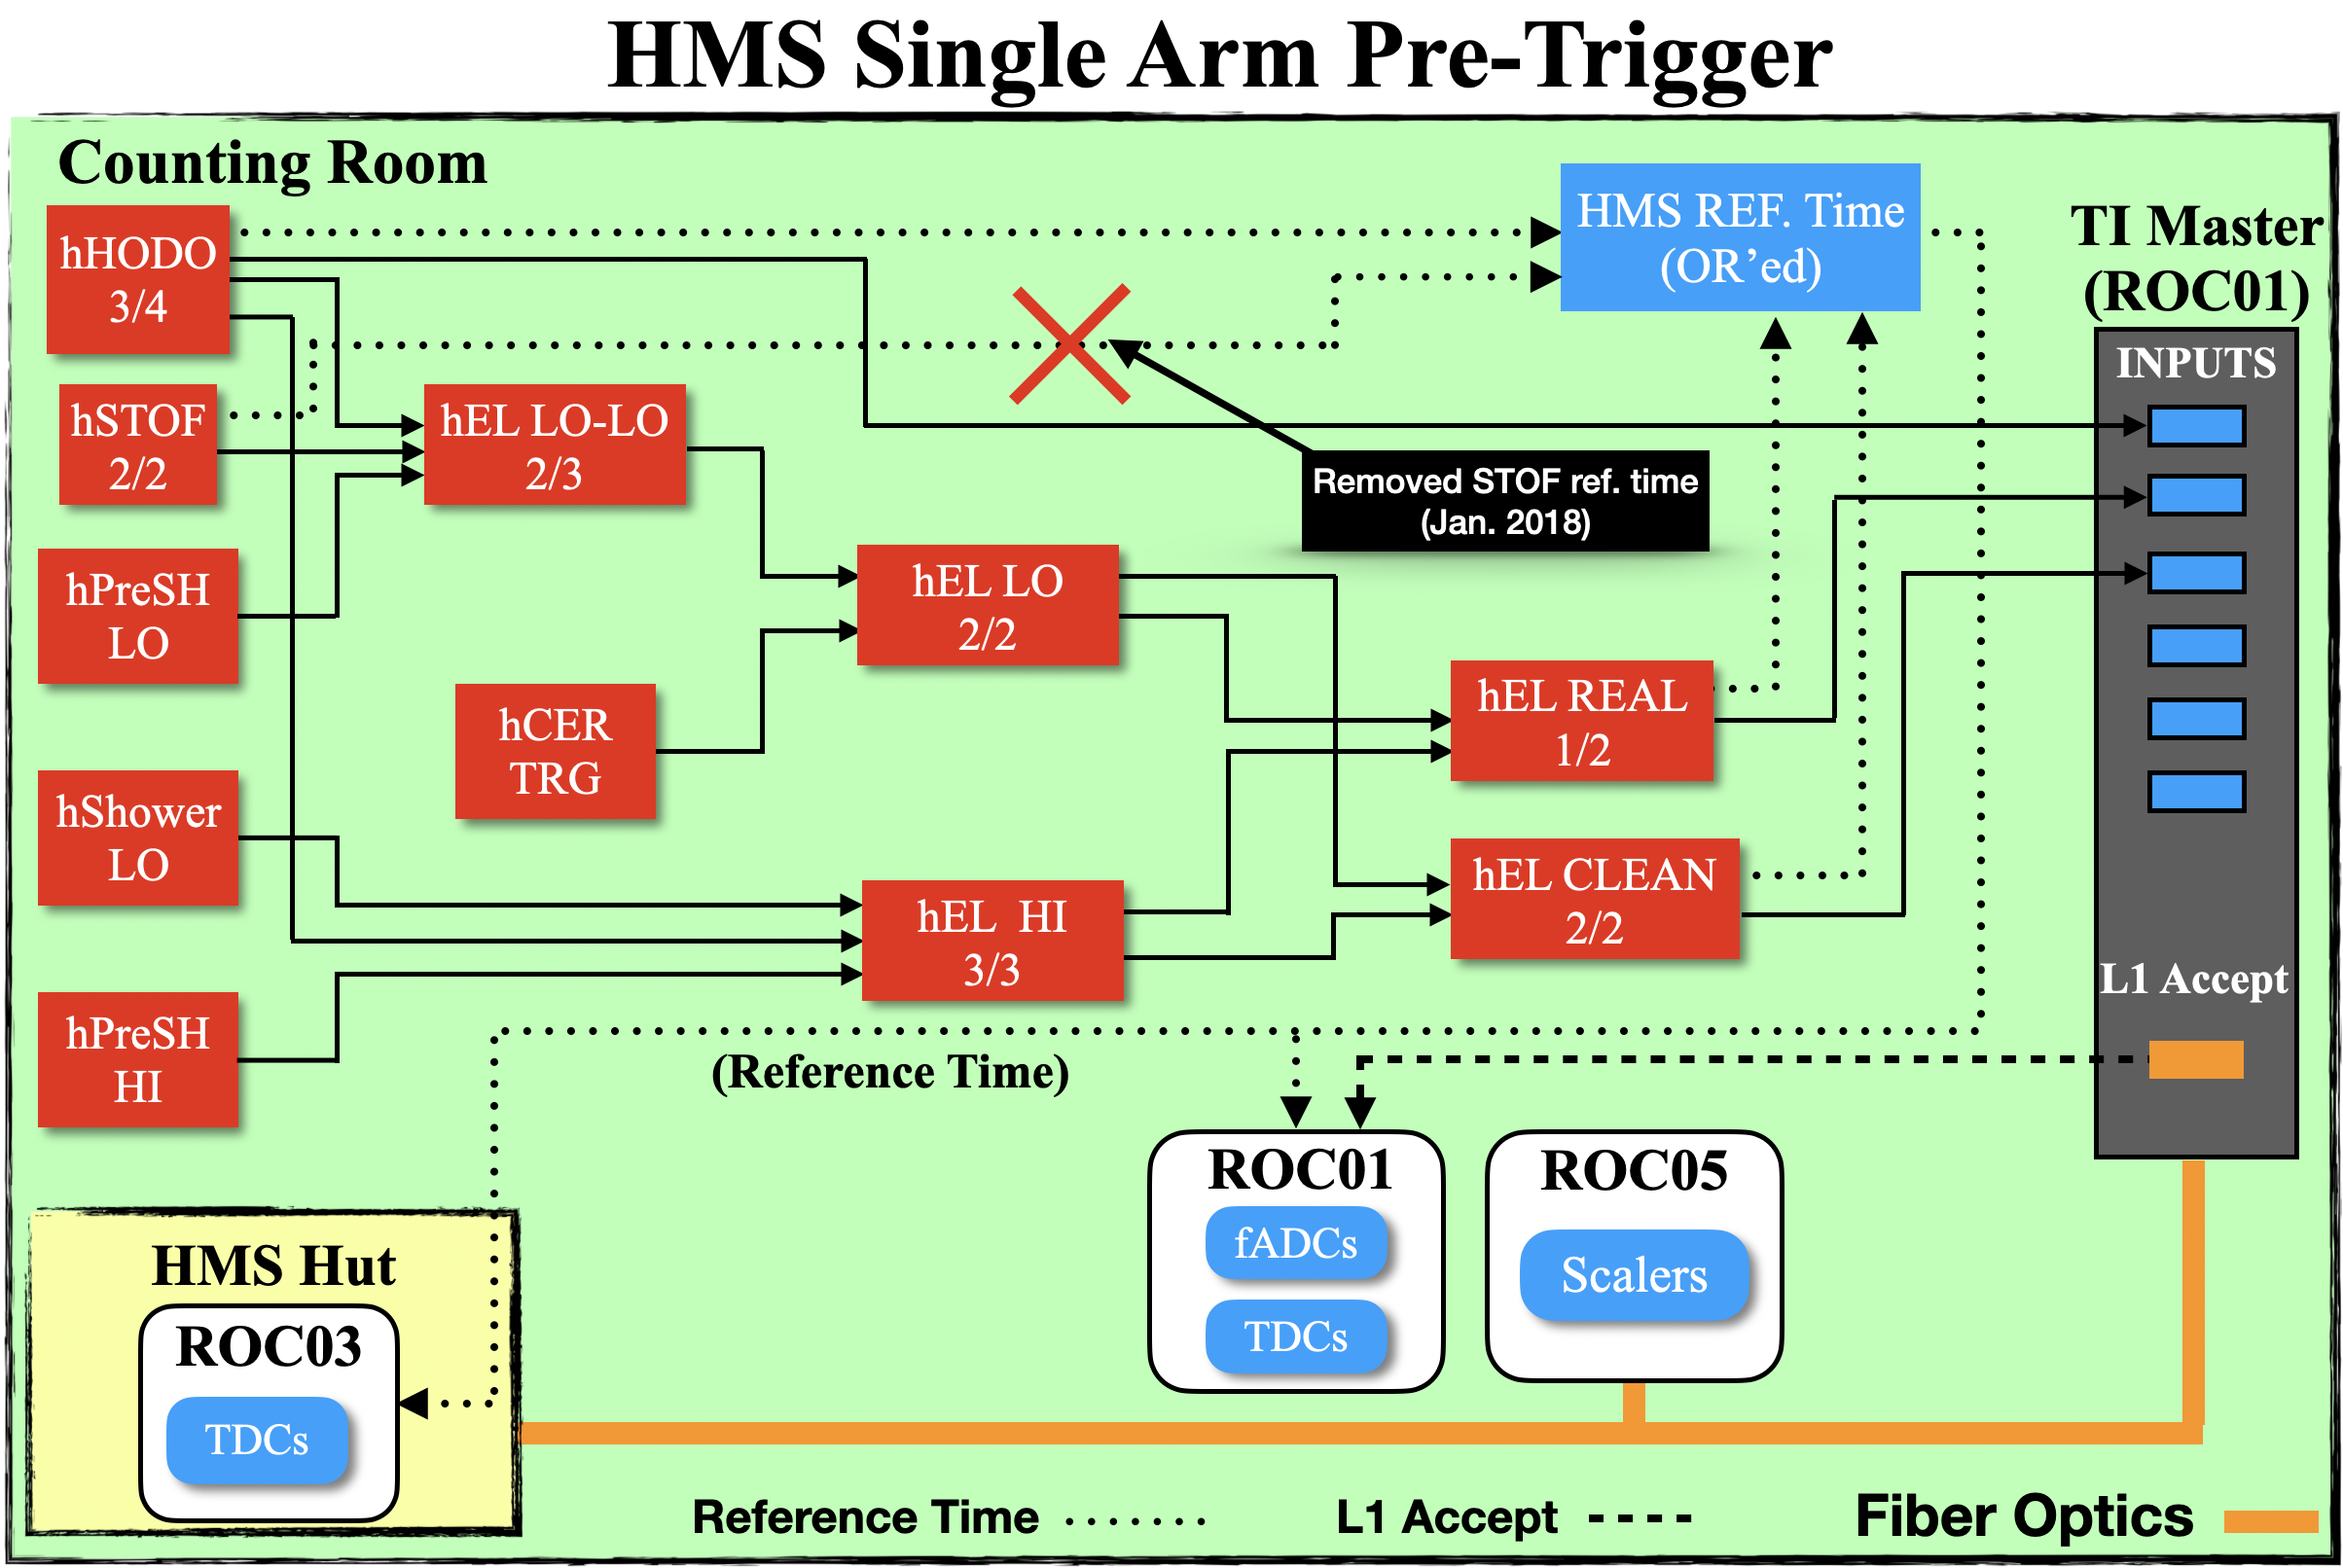
\includegraphics[scale=0.38]{./Jan2018_trigger_change.png}
  \caption{The STOF was removed from the reference time definition in both spectrometers (HMS/SHMS) on January 23, 2018. See HC-Log Entry (for HMS):\url{https://logbooks.jlab.org/entry/3519686}. Note: The trigger
  electronics is shown for HMS, but also applies to the SHMS.}
  \label{fig:stof_refTime_remove}
\end{figure}
On January 2018, the STOF reference time was removed from the original reference time definition (see Eq.\ref{eq:refTime_def1}), and the reference time was redefined as
\begin{align}
  T^{\mathrm{logic}}_{\mathrm{reftime,Jan18}} \equiv &\textbf{ p(h)HODO 3/4} \text{ OR } \textbf{p(h)EL-REAL} \text{ OR } \textbf{p(h)EL-CLEAN}
  \label{eq:refTime_def2}
\end{align}
\subsection{August, 2018: Removal of EL-CLEAN from Reference Time Definition}\label{ssec:aug2018}
\begin{figure}[H]
  \centering
  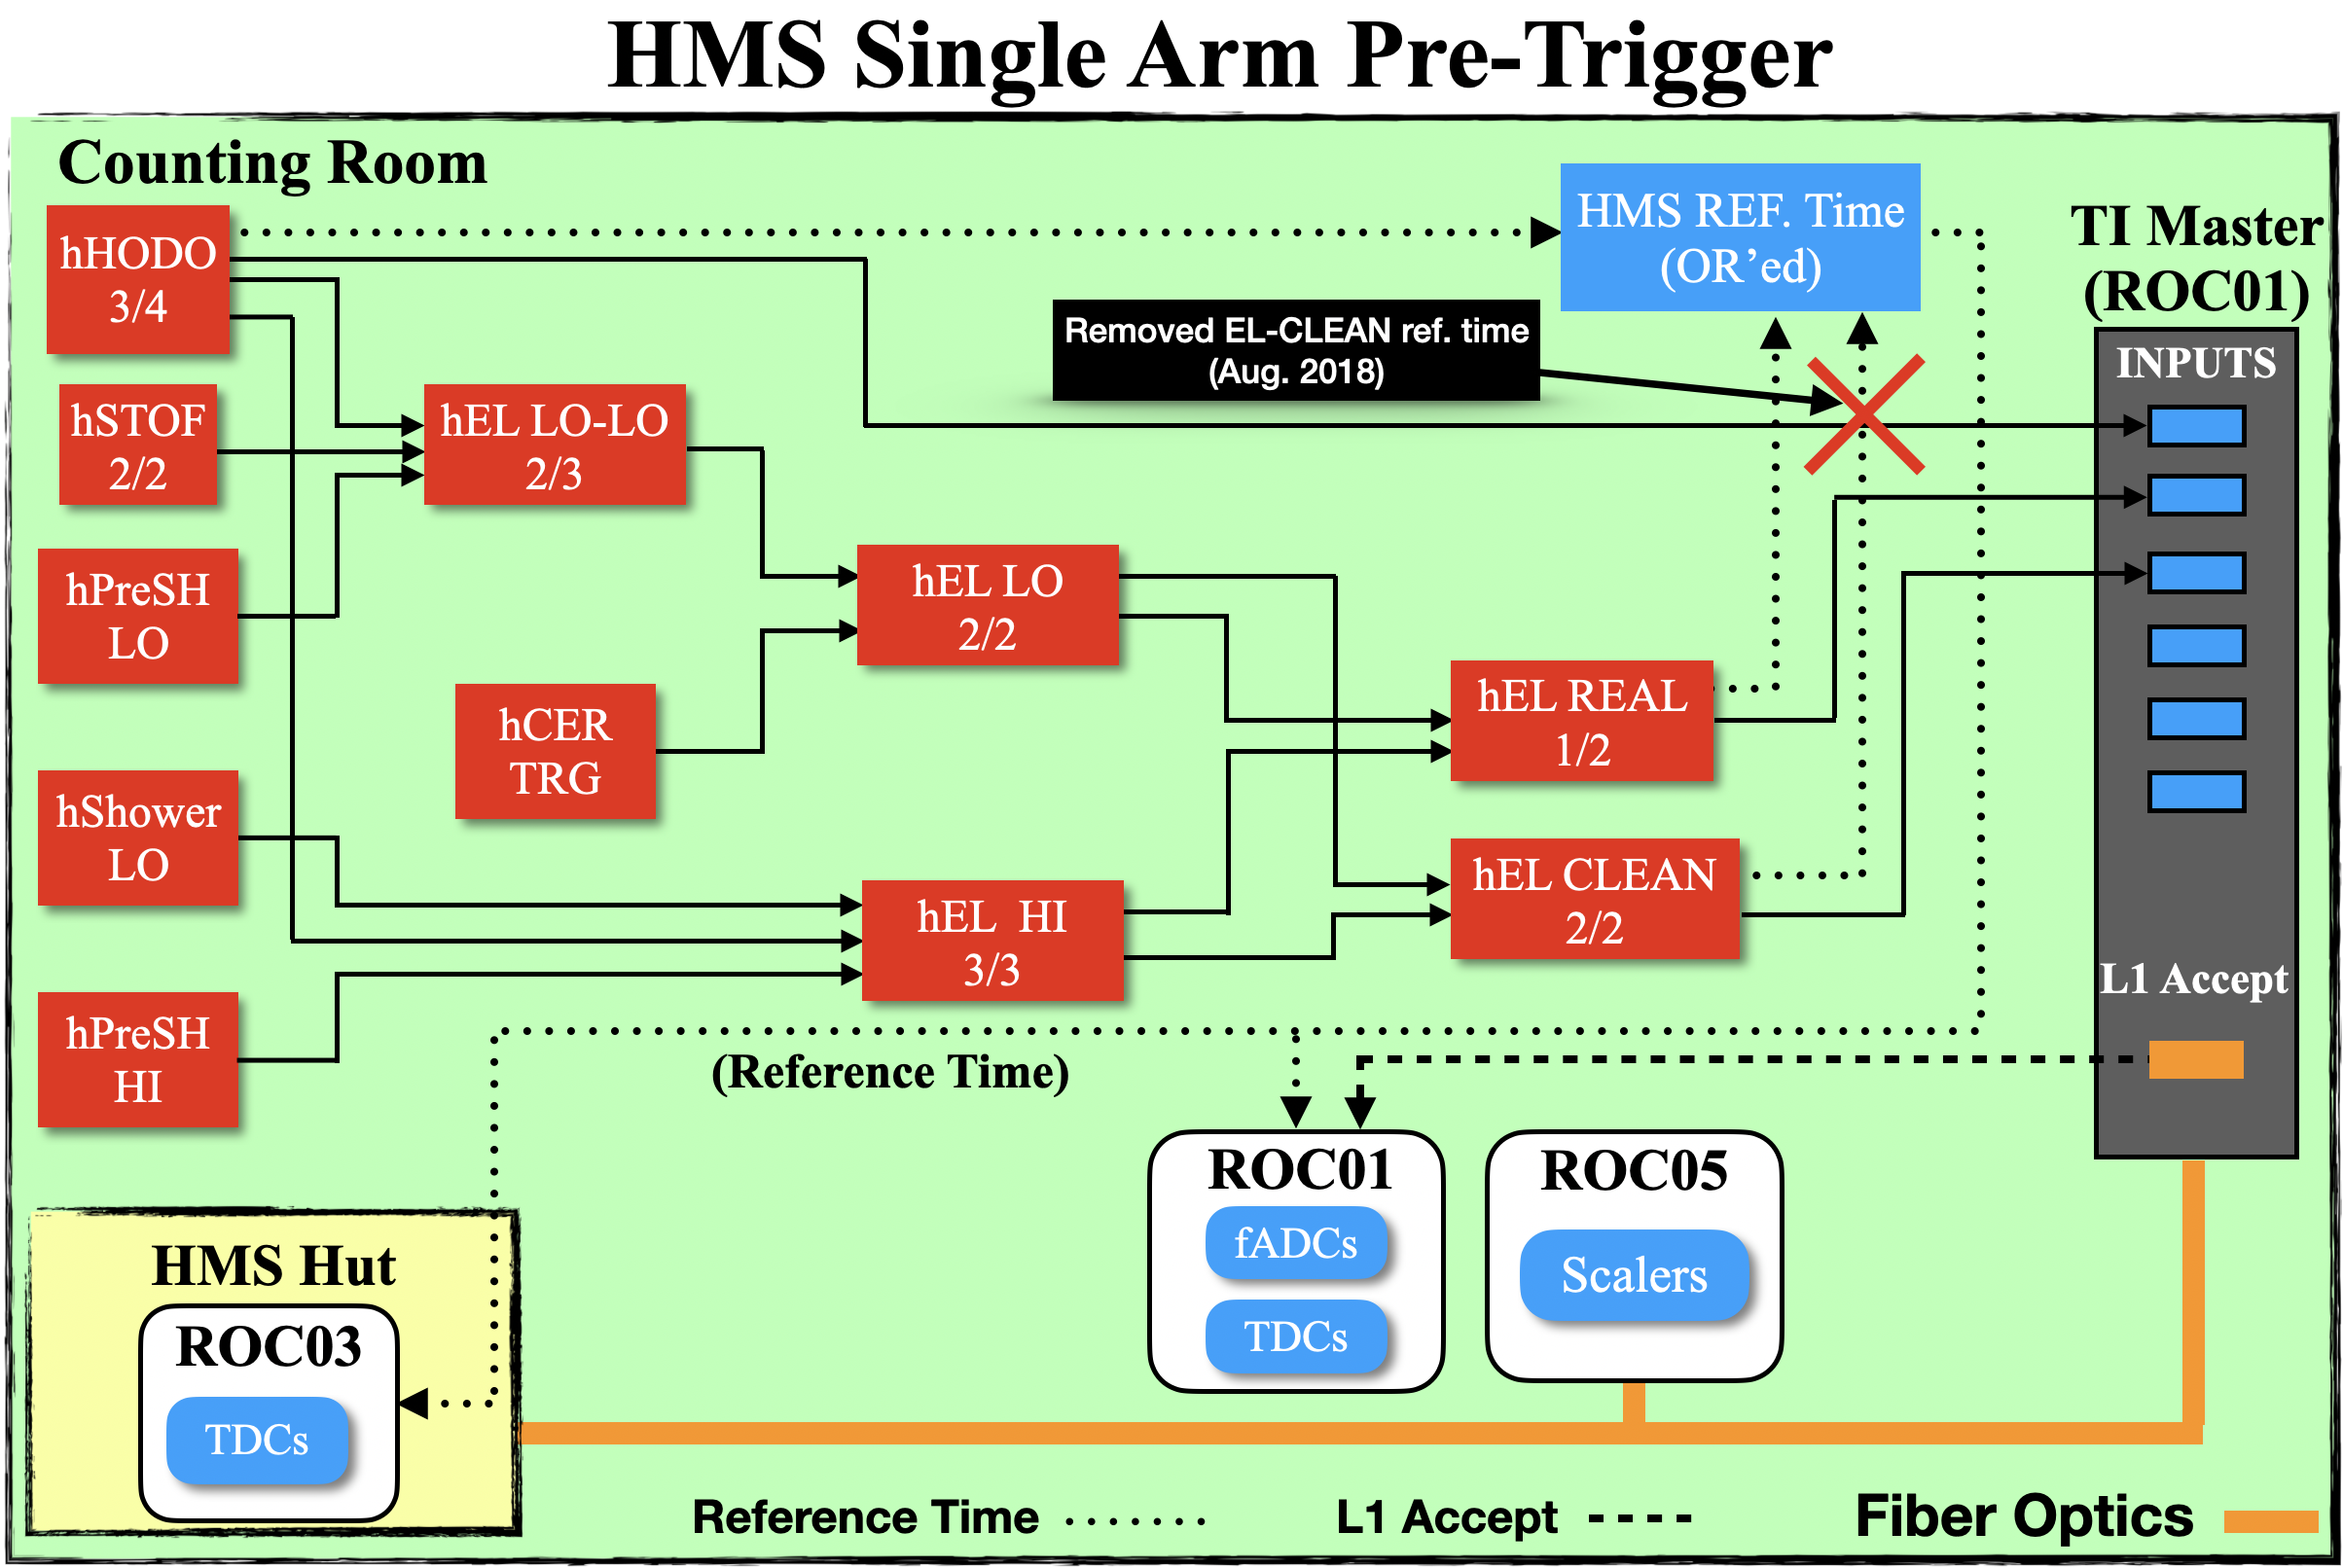
\includegraphics[scale=0.38]{./Aug2018_trigger_change.png}
  \caption{The EL-CLEAN was removed from the reference time definition in both spectrometers (HMS/SHMS) on August 09, 2018. See HC-Log Entry:\url{https://logbooks.jlab.org/entry/3585301}. Note: The trigger
  electronics is shown for HMS, but also applies to the SHMS.}
  \label{fig:elclean_refTime_remove}
\end{figure}
On August 2018, EL-CLEAN was removed from the reference time definition. It was determined that any pre-trigger that required the HODO 3/4 was unnecessary and redundant to have in the
reference time definition so it was removed. The reference time was redefined once again as follows:
\begin{align}
  T^{\mathrm{logic}}_{\mathrm{reftime,Aug18}} \equiv &\textbf{ p(h)HODO 3/4} \text{ OR } \textbf{p(h)EL-REAL}
  \label{eq:refTime_def3}
\end{align}
\subsection{December, 2019: Removal of STOF from trigger / Removal of EL-REAL from Reference Time Definition}\label{ssec:dec2019}
\begin{figure}[H]
  \centering
  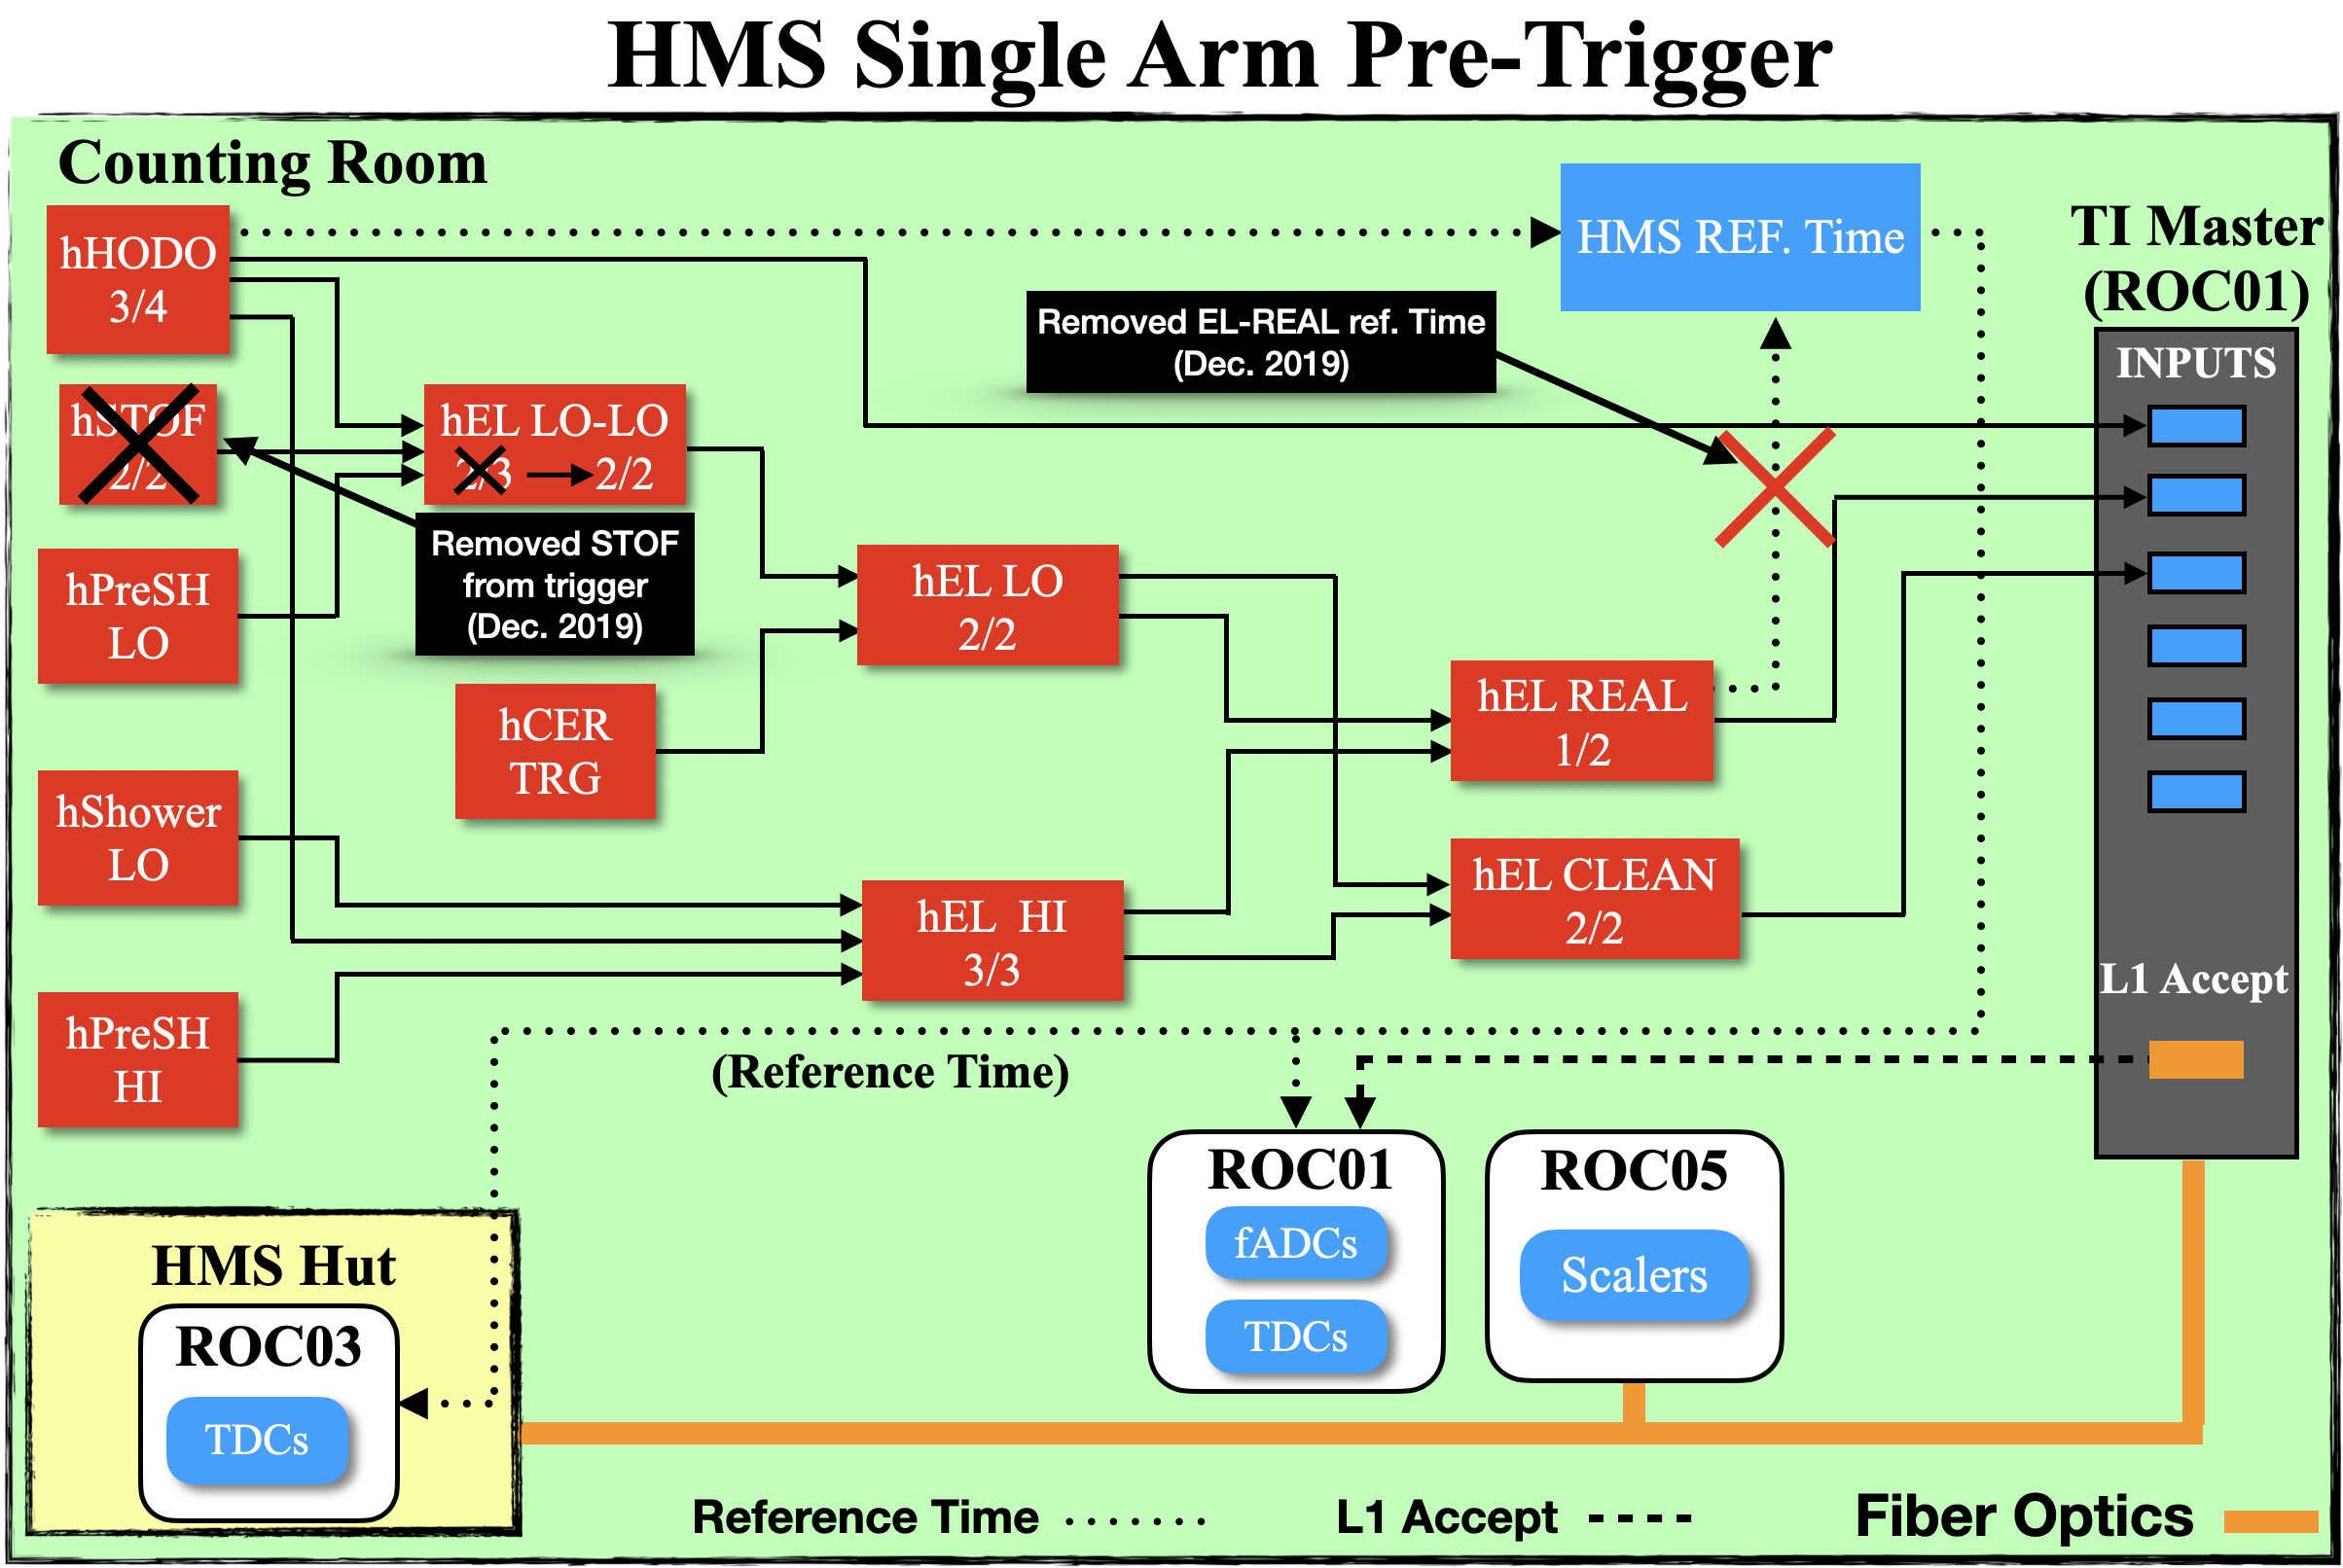
\includegraphics[scale=0.38]{./Dec2019_trigger_change.png}
  \caption{The STOF was removed from electronics trigger and EL-REAL was removed from the reference time definition in both spectrometers (HMS/SHMS) on Dec 06, 2019. See the \textit{highlights} section of
    HC-Log Entry:\url{https://logbooks.jlab.org/entry/3747761}. Note: The trigger
  electronics is shown for HMS, but also applies to the SHMS.}
  \label{fig:elreal_refTime_remove}
\end{figure}
\indent On early December 2019, before the start of the A1n/d2n experimental run periods, the STOF was removed from the trigger definition in both spectrometers.
Since STOF trigger was removed, the EL-REAL now requires a HODO 3/4 and it was determined that this reference time (EL-REAL) was no longer needed so it was removed
from the reference time definition as well. The reference time was redefined as follows:
\begin{align}
  T^{\mathrm{logic}}_{\mathrm{reftime,Dec19}} \equiv &\textbf{ p(h)HODO 3/4}
  \label{eq:refTime_def4}
\end{align}
\newpage
\subsection{Electronics Trigger Oscilloscope Traces}\label{ssec:traces}
For a visual representation of the trigger logic signals discussed, see a summary of the various trigger oscilloscope traces taken since the start of the commissioning phase:\\
\newline
\noindent \textbf{December 2017:}\\
SHMS: \url{https://logbooks.jlab.org/entry/3508587}\\
HMS: \url{https://logbooks.jlab.org/entry/3504470}\\

\noindent \textbf{September 2018:}\\
SHMS: \url{https://logbooks.jlab.org/entry/3599311}\\
HMS: \url{https://logbooks.jlab.org/entry/3599283}\\

\noindent \textbf{February 2019:}\\
SHMS: \url{https://logbooks.jlab.org/entry/3655622}\\
HMS: \url{https://logbooks.jlab.org/entry/3655644}\\

\noindent \textbf{December 2019:}\\
SHMS: \url{https://logbooks.jlab.org/entry/3752072}\\
HMS: \url{https://logbooks.jlab.org/entry/3752087}\\


\newpage
\onecolumn
\bibliography{trigger_v3}
\bibliographystyle{acm}

\newpage
\begin{appendices}
\appendix
\section{Original Electronics Diagrams}
\subsection{HMS Hodoscopes Electronics Diagram}
\label{appendix:AppxA1}
\begin{figure}[h!]
  \centering
  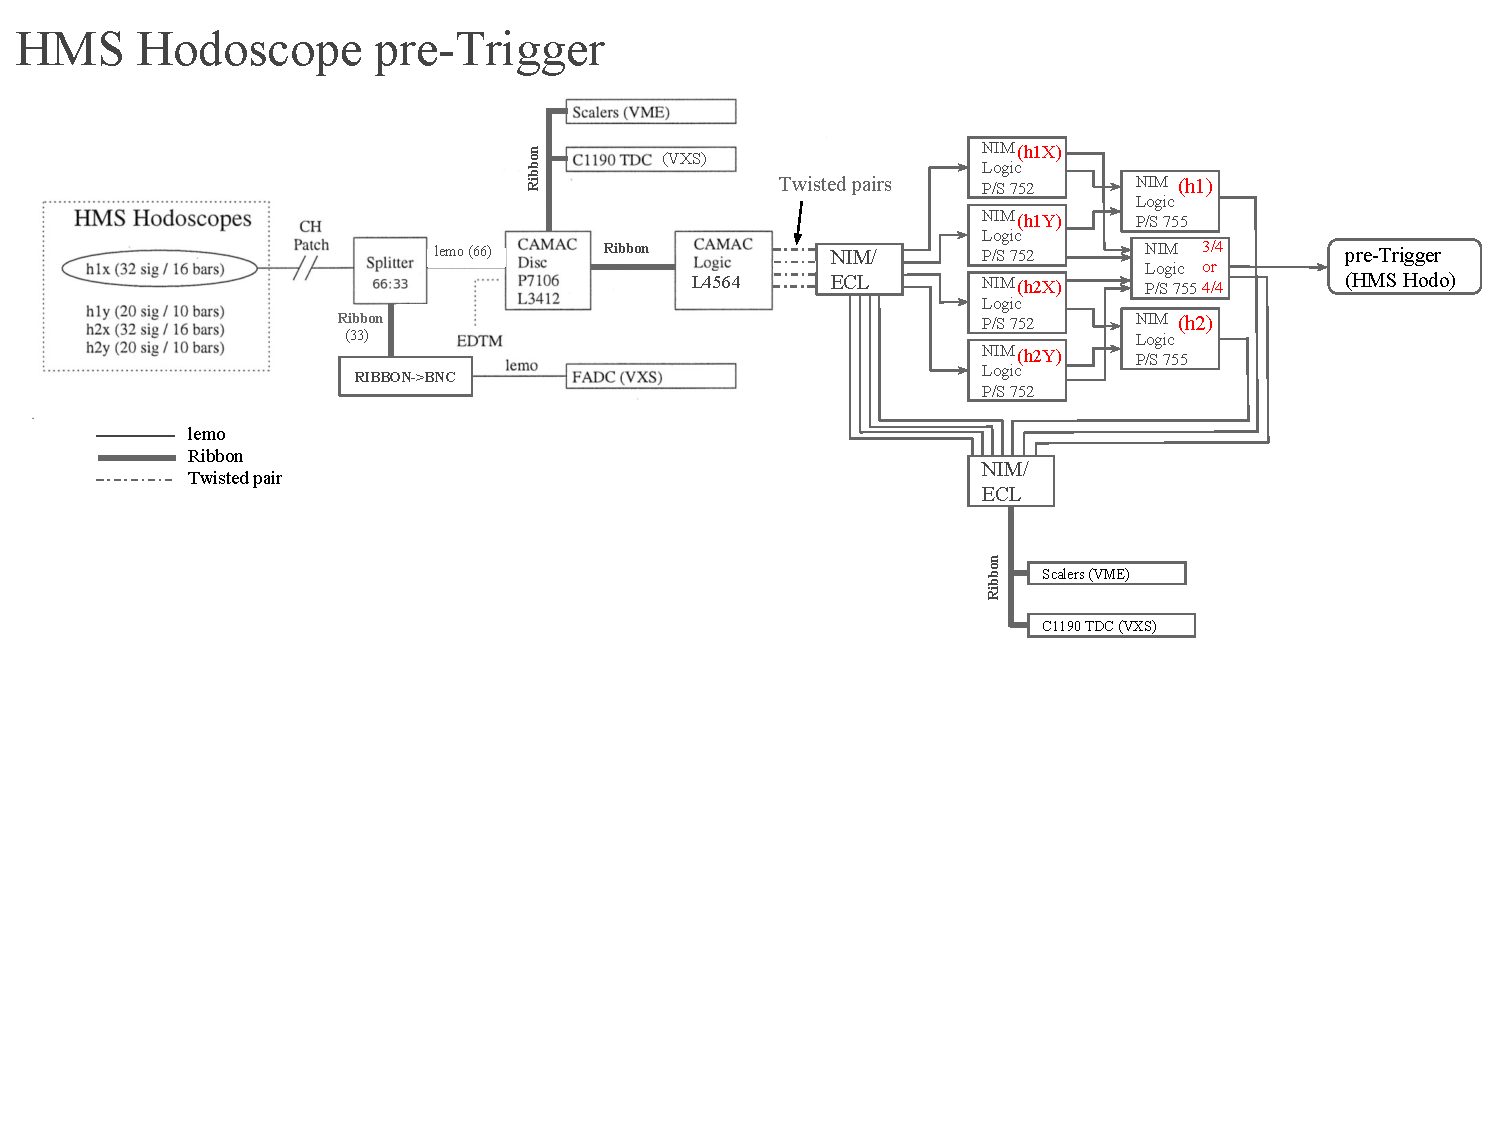
\includegraphics[width=7.0in, height=3.2in]{../HMS_HODO_TRIGGER.pdf}
  \caption{Original HMS Hodoscopes Electronics Diagram.}
  \label{fig:hms_hod_trg}
\end{figure}
\subsection{HMS Calorimeter Electronics Diagram}
\label{appendix:AppxA2}
\begin{figure}[h!]
  \centering
  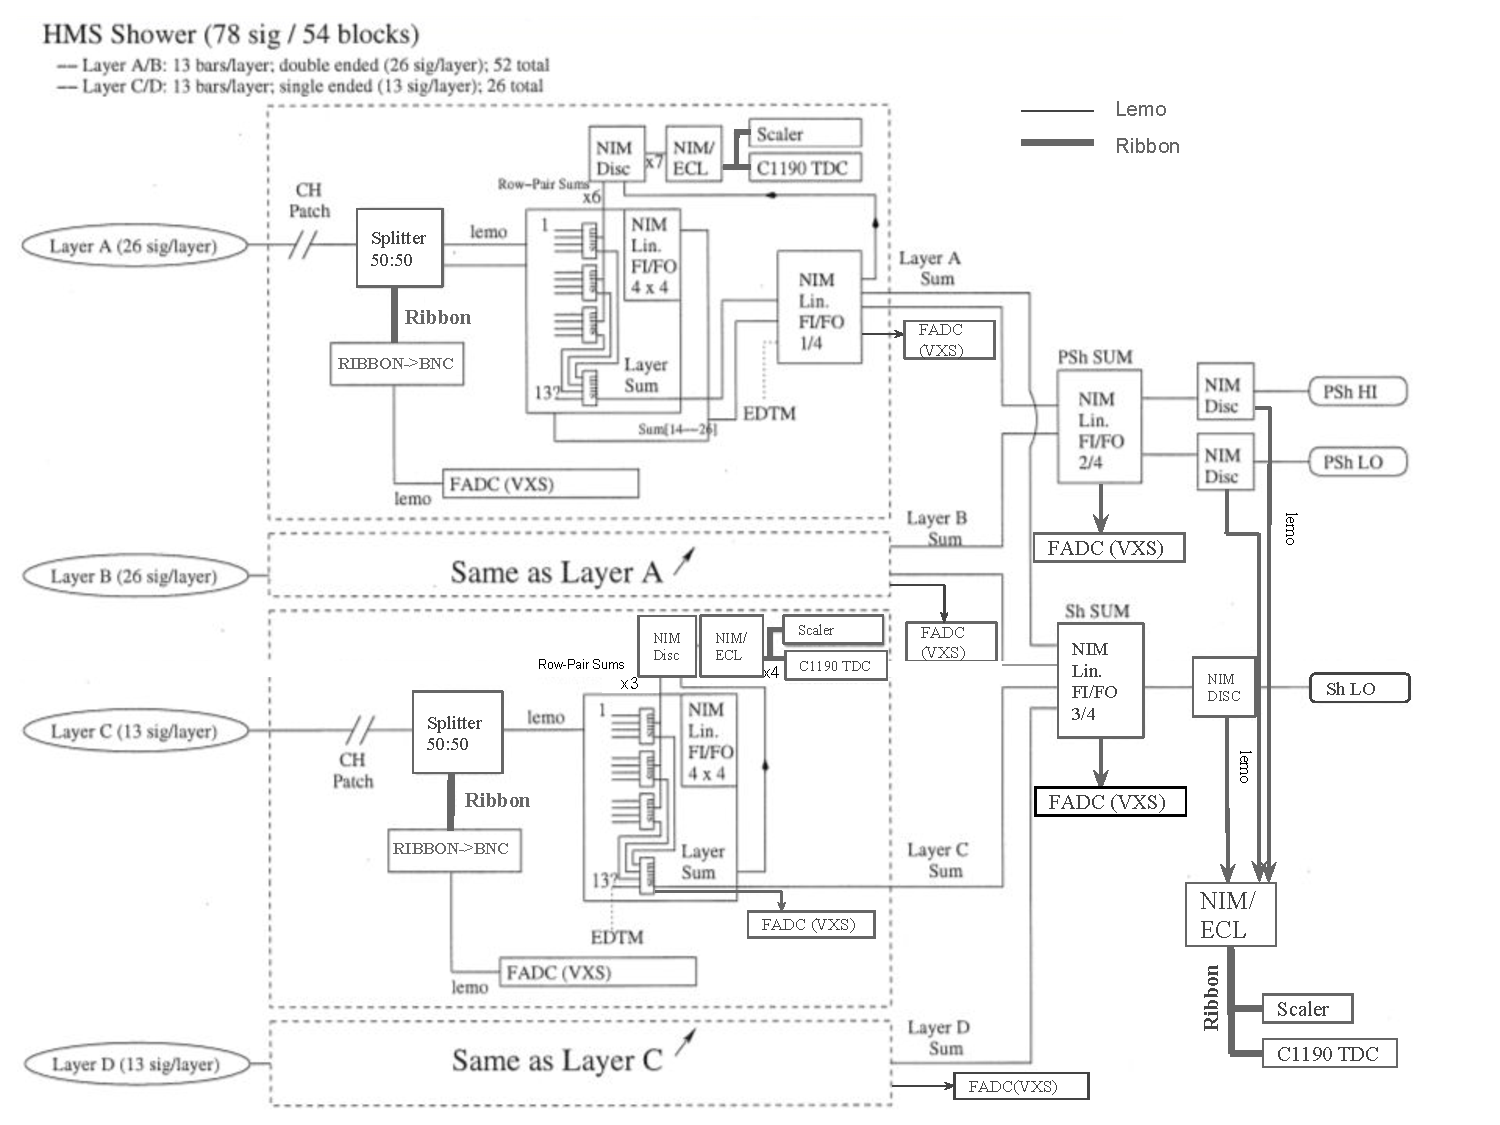
\includegraphics[width=6.in, height=4.in]{../HMS_Cal_Trigger.pdf}
  \caption{Original HMS Calorimeter Electronics Diagram.}
  \label{fig:hms_cal_trg}
\end{figure}

\subsection{HMS Gas \v{C}erenkov Electronics Diagram}
\label{appendix:Appx3}
\begin{figure}[h!]
  \centering
  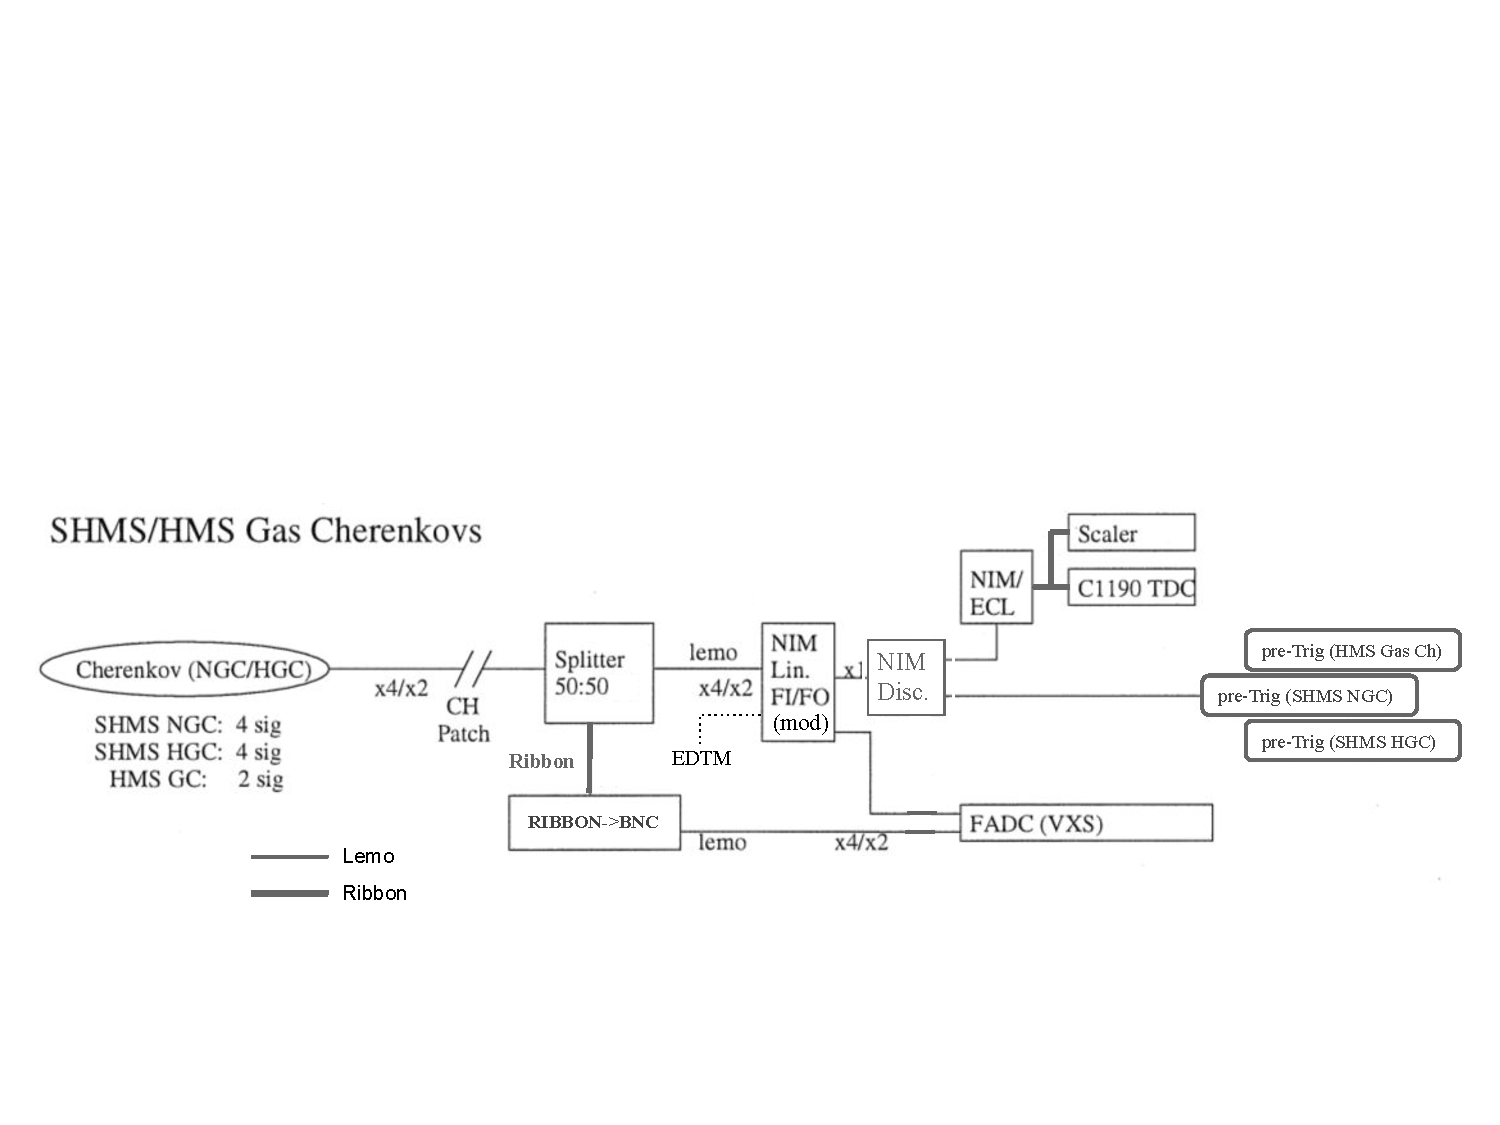
\includegraphics[width=7.0in, height=2.0in]{../HMS_Cer_trig.pdf}
  \caption{Original HMS Gas \v{C}erenkov Electronics Diagram. Same electronics diagram applies for SHMS Gas \v{C}erenkov.}
  \label{fig:hms_gas_cer_trg}
\end{figure}

\subsection{HMS Aerogel \v{C}erenkov Electronics Diagram}
\label{appendix:Appx4}
\begin{figure}[h!]
  \centering
  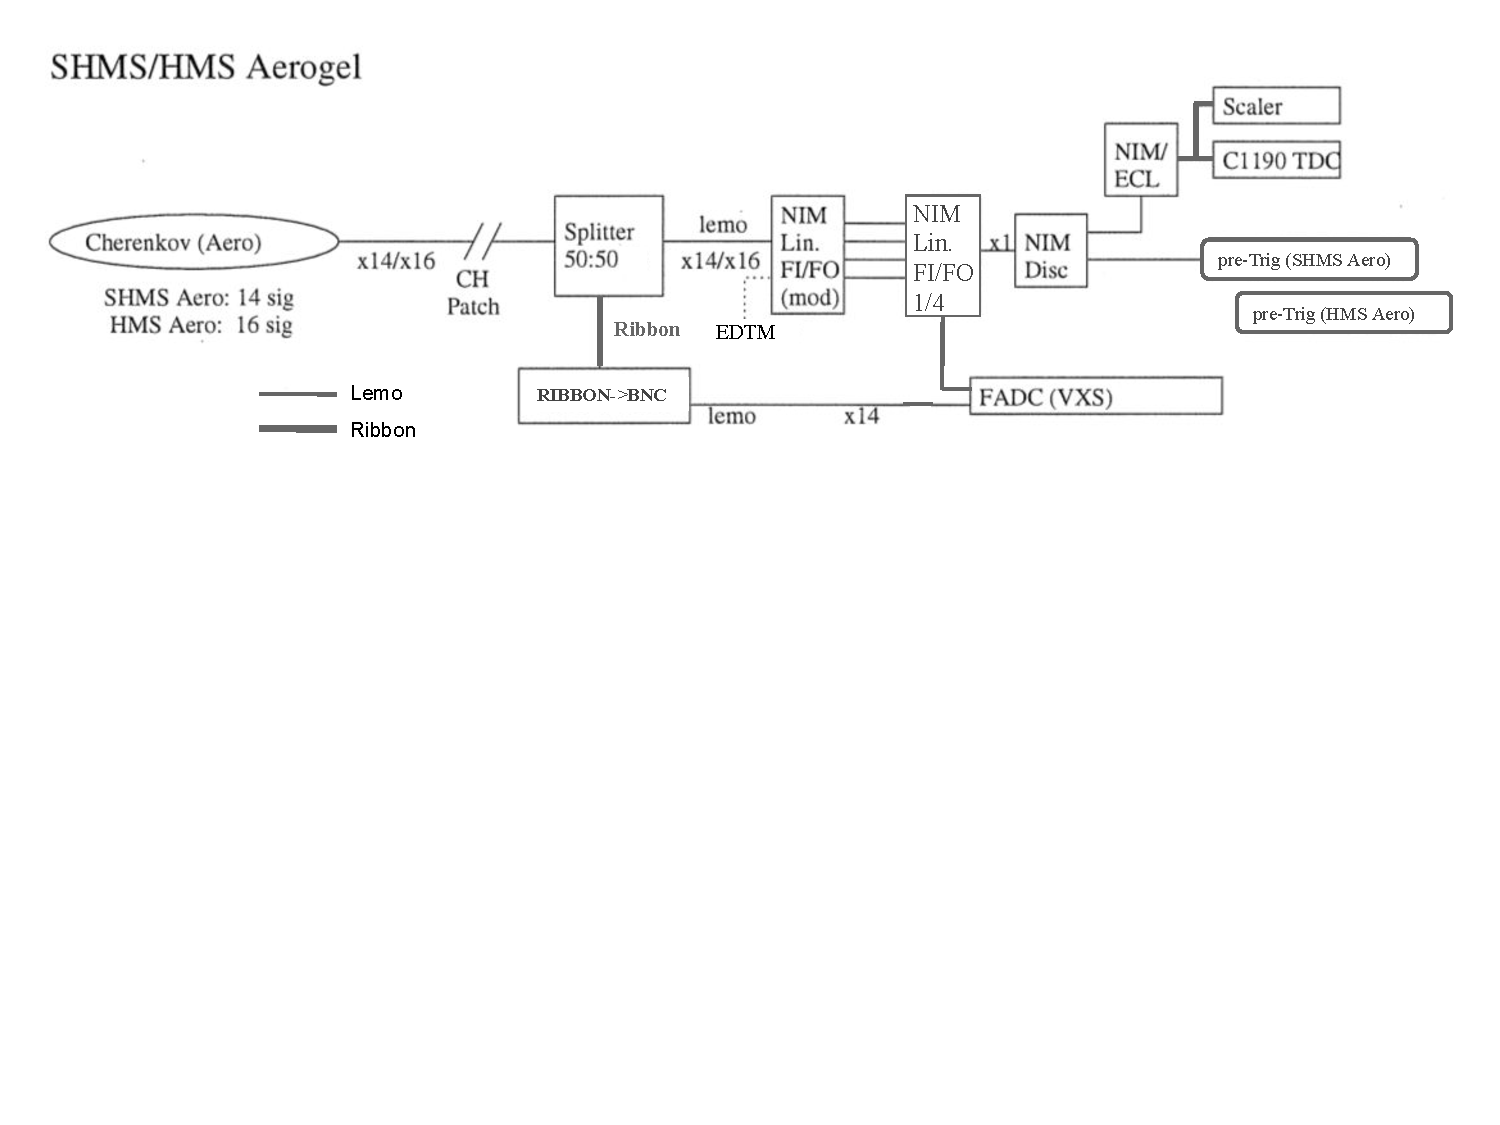
\includegraphics[width=6.5in, height=2.1in]{../HMS_Aero_trig.pdf}
  \caption{Original HMS Gas \v{C}erenkov Electronics Diagram. Same electronics diagram applies for SHMS Gas \v{C}erenkov.}
  \label{fig:hms_gas_cer_trg}
\end{figure}
\newpage
\subsection{HMS Single Arm Electronics Diagram}
\label{appendix:Appx5}
\begin{figure}[h!]
  \centering
  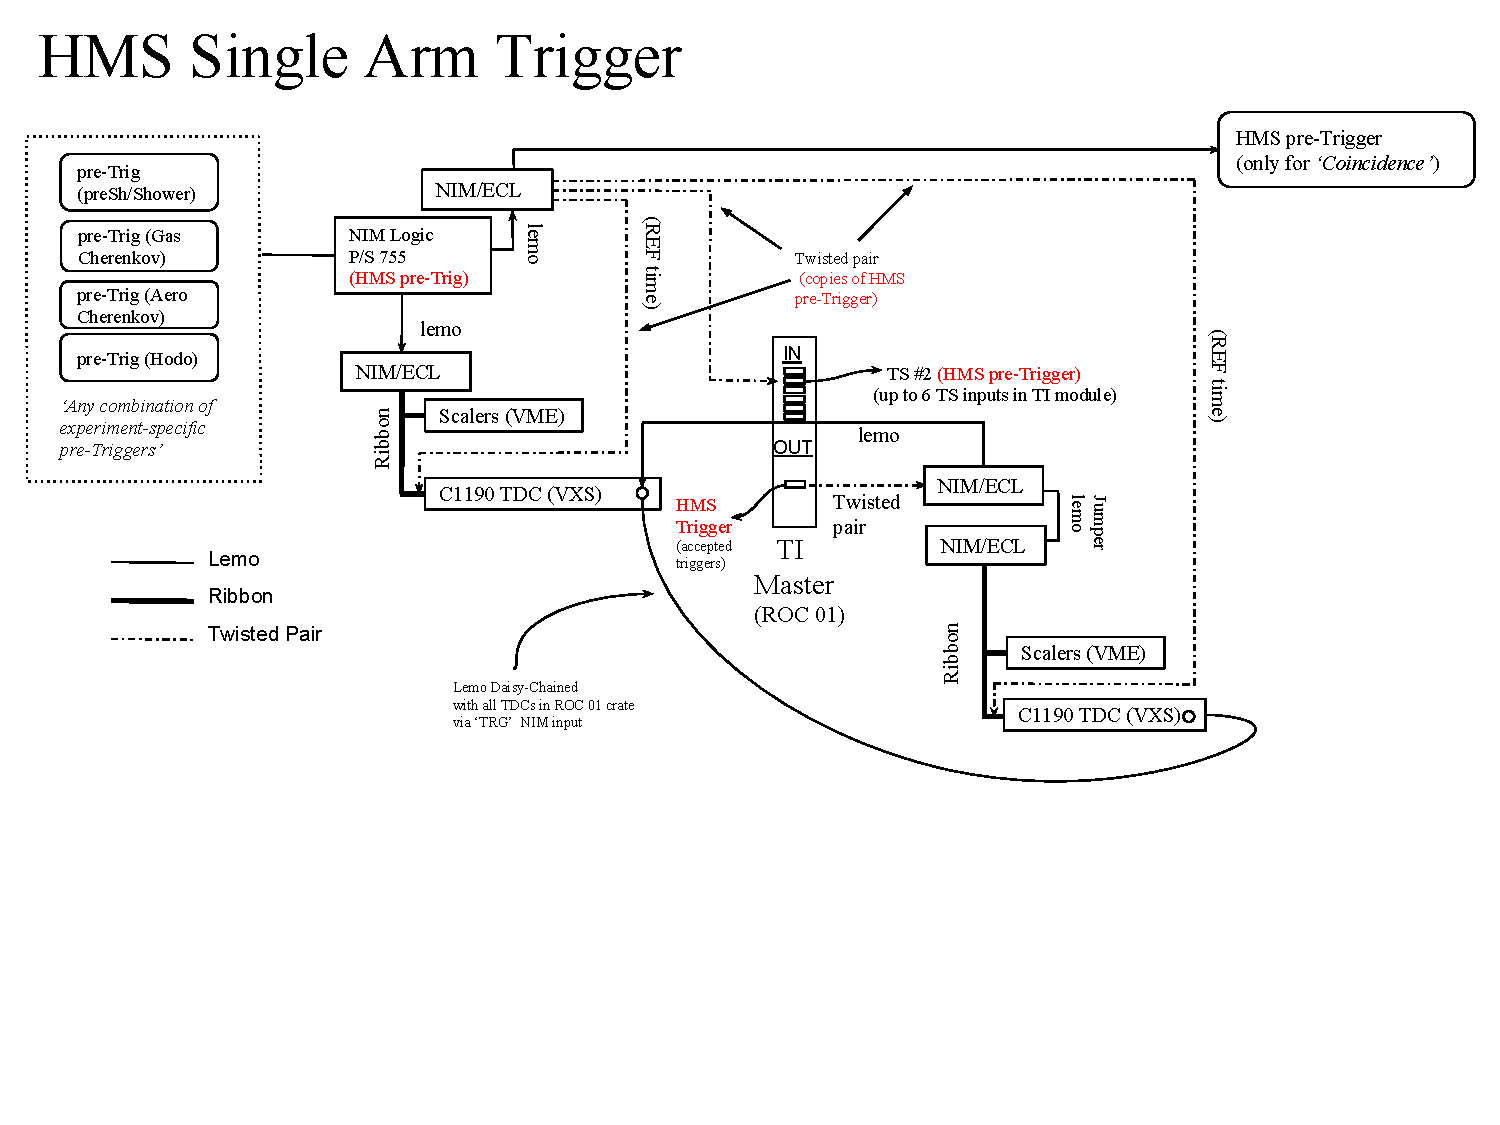
\includegraphics[width=7.0in, height=3.8in]{../HMS_SingleArm_Trigger.pdf}
  \caption{Original HMS Single Arm Trigger Electronics Diagram.}
  \label{fig:hms_one_arm_trg}
\end{figure}
\subsection{SHMS Hodoscopes Pre-Trigger}
\label{appendix:Appx6}
\begin{figure}[h!]
  \centering
  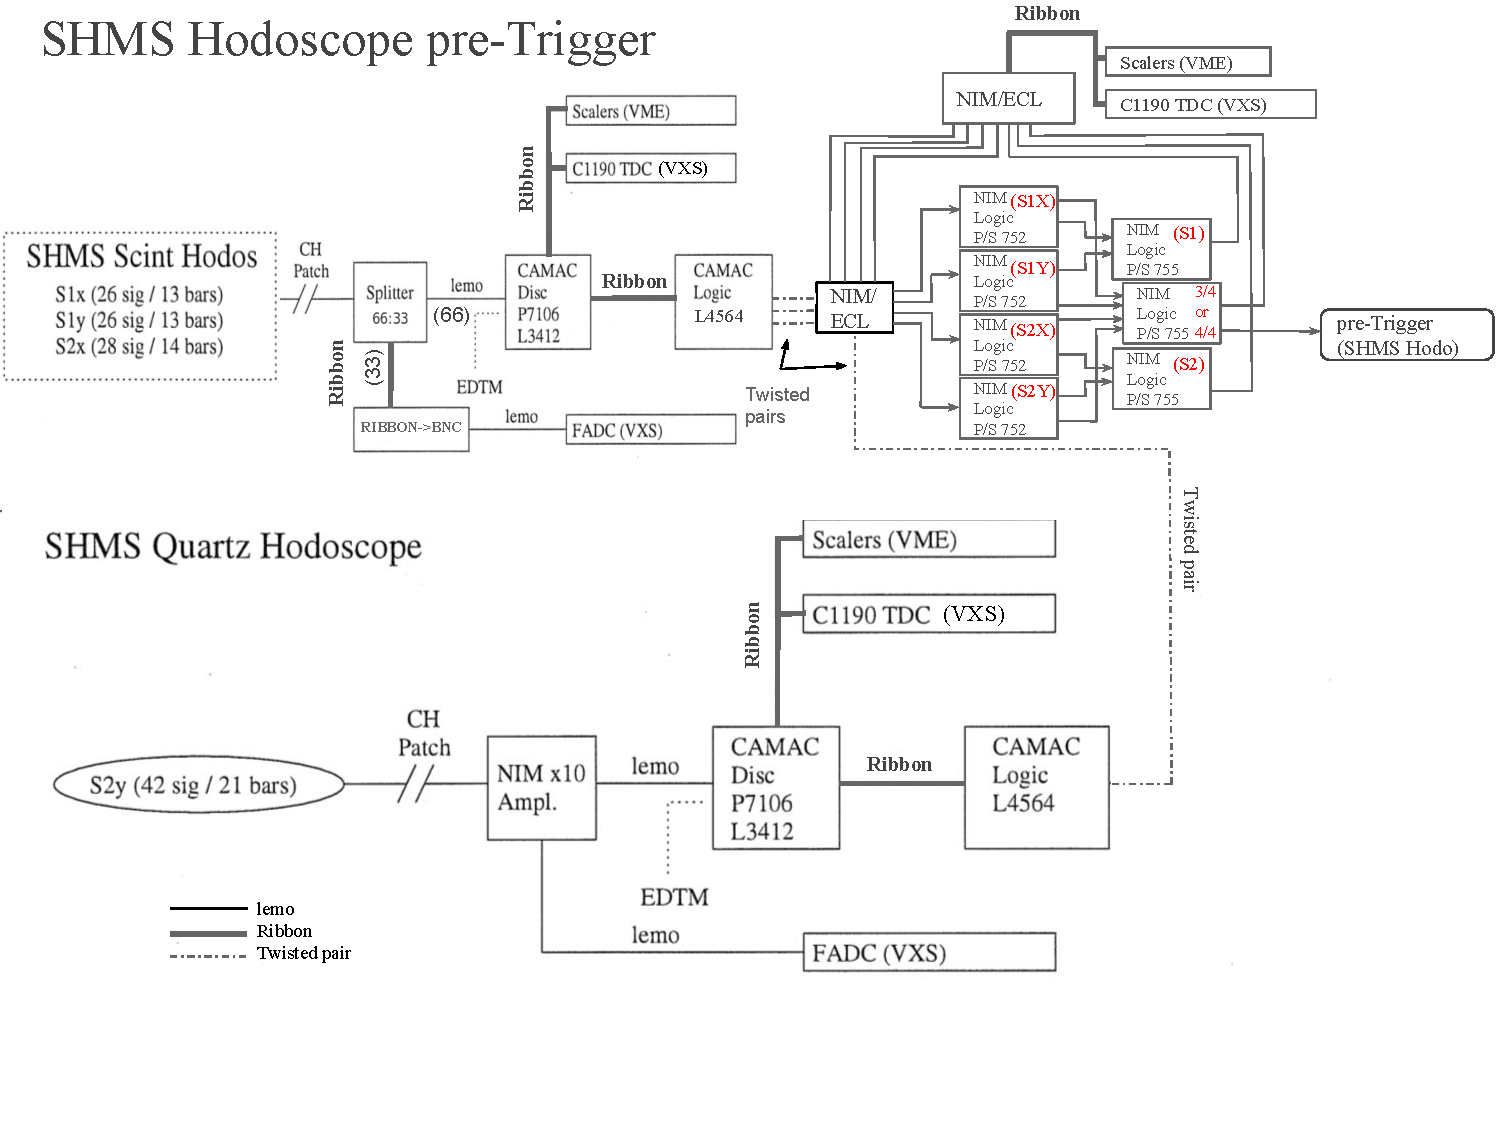
\includegraphics[width=6.8in, height=3.9in]{../SHMS_HODO_TRIGGER.pdf}
  \caption{Original SHMS Hodoscope Electronics Diagram.}
  \label{fig:shms_hod_trg}
\end{figure}
\newpage
\subsection{SHMS Pre-Shower / Shower Calorimeter Pre-Trigger}
\label{appendix:Appx7}
\begin{figure}[h!]
  \centering
  \includegraphics[width=7.0in, height=3.0in]{../SHMS_preSh_trigger.pdf}
  \caption{Original SHMS PreShower Electronics Diagram}
  \label{fig:shms_preSh_trg}
\end{figure}
\subsection{SHMS Single Arm Pre-Trigger}
\label{appendix:Appx8}
\begin{figure}[h!]
  \centering
  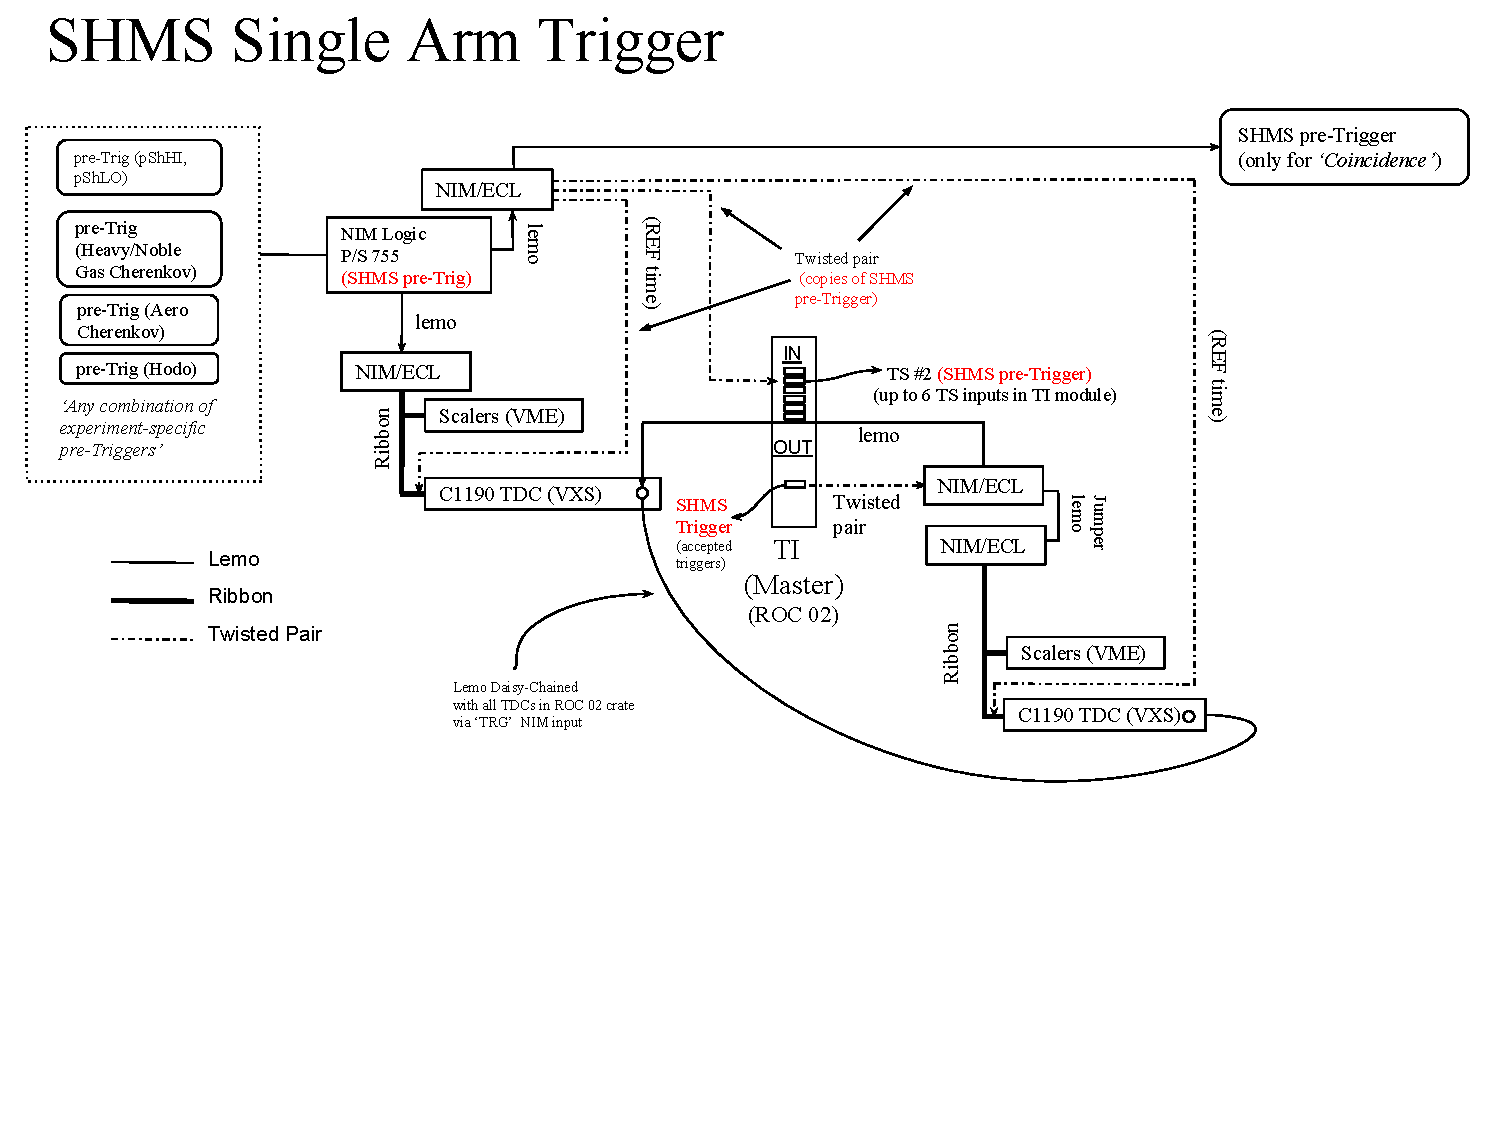
\includegraphics[width=7.0in, height=3.8in]{../SHMS_SingleArm_Trigger.pdf}
  \caption{Original SHMS Single Arm Trigger Electronics Diagram}
  \label{fig:shms_one_arm_trg}
\end{figure}
\newpage
\subsection{Coincidence Pre-Trigger}
\label{appendix:Appx9}
\begin{figure}[h!]
  \centering
  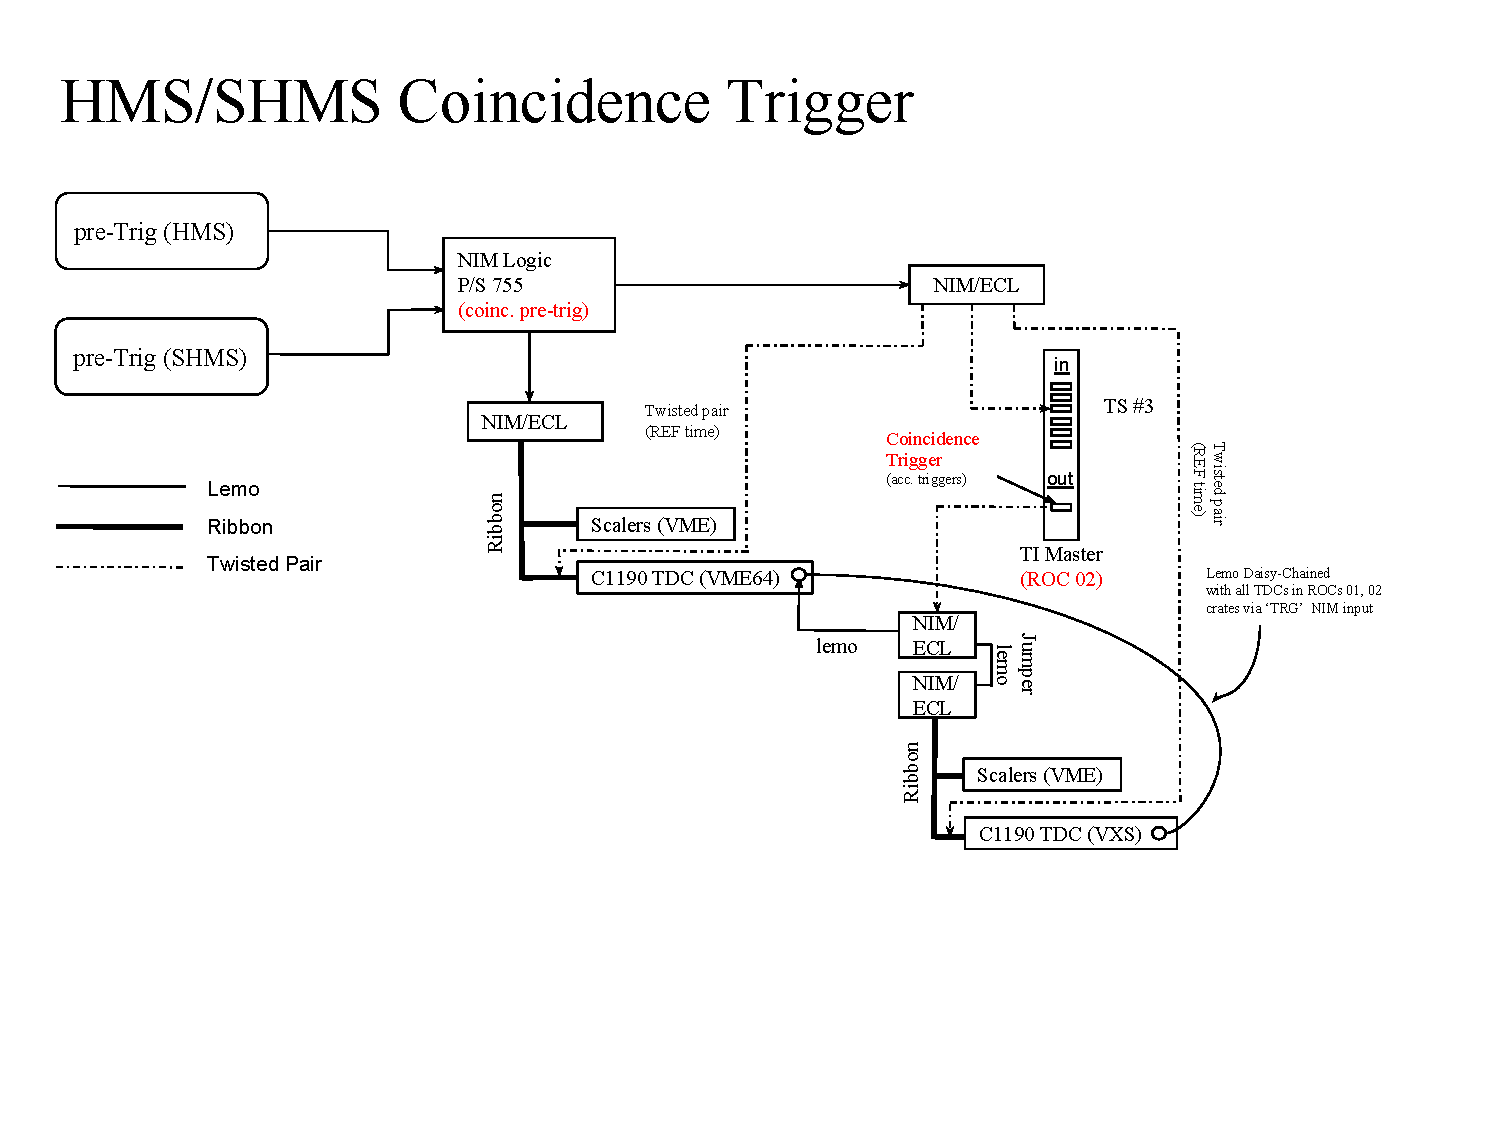
\includegraphics[width=7.0in, height=3.8in]{../Coincidence_Trigger.pdf}
  \caption{Original Coincidence Trigger Electronics Diagram}
  \label{fig:coin_trg}
\end{figure}


\end{appendices}

\end{document}
